%%%%%%%%%%%%%%%%%%%%%%%%%
% Dokumentinformationen %
%%%%%%%%%%%%%%%%%%%%%%%%%
\newcommand{\titleinfo}{ProgCPP\_ZF FS18}
\newcommand{\authorname}{\href{mailto:noah.kaelin@hsr.ch}{N. Kaelin}}
\newcommand{\authoremail}{\href{mailto:noah.kaelin@hsr.ch}{noah.kaelin@hsr.ch} }
\newcommand{\versioninfo}{$ V1.0 $}

%%%%%%%%%%%%%%%%%%%%%%%%%%%%%%%%%%%%%%%%%%%%%
% Standard Header für 
% - Makros 
% - Farben
% - Mathematische Operatoren
%%%%%%%%%%%%%%%%%%%%%%%%%%%%%%%%%%%%%%%%%%%%%
%BuG-Fix
%Package pdf Error: Driver file ................ not found
%If you have a luatex driver fail uncomment these lines
%\RequirePackage{luatex85}
%\def\pgfsysdriver{pgfsys-pdftex.def}

% Genereller Header
\documentclass[11pt,twoside,a4paper,fleqn]{article}
% Dateiencoding
\usepackage[utf8]{inputenc}
\usepackage[T1]{fontenc}	%ä,ü...
% Seitenränder
\usepackage[left=1cm,right=1cm,top=0.5cm,bottom=0.2cm,includeheadfoot]{geometry}
\setlength{\headsep}{5pt} 
% Sprachpaket 
\usepackage[english, ngerman]{babel} % Silbentrennung und Rechtschreibung Englisch und Deutsch

%%%%%%%%%%%%%%%%%%%%%%%
%% Wichtige Packages %%
%%%%%%%%%%%%%%%%%%%%%%%
\usepackage{amsmath}                % Allgemeine Matheumgebungen									
%\usepackage{amssymb}                % Fonts: msam,msbm, eufm & Mathesymbole, Mengen (lädt automatisch amsfonts)									
\usepackage{array}                  % \newcolumntype, \firsthline, ,\lasthline, m{width}, b{width}									
\usepackage{caption}                % Bildunterschriften									
\usepackage{enumitem}               % basic environments: enumerate, itemize, description									
\usepackage{fancybox}               % \fbox: \shad­ow­box, \dou­ble­box, \oval­box, \Oval­box									
\usepackage{fancyhdr}               % Seiten schöner gestalten, insbesondere Kopf- und Fußzeile									
\usepackage{floatflt}               % Textumflossene Abbildungen \begin{floatingfigure}[r]{Breite} : r rechts, l links, p links auf geraden Seiten und rechts auf ungeraden Seiten								
\usepackage{graphicx}               % \includegraphics[keyvals]{imagefile}, [draft]graphicx zeigt nur Namen und Rahmen an, [final] hebt diese option auf => Bild wird angezeigt    									
\usepackage{hyperref}               % Erstellt Verweise innerhalb und nach außerhalb eines PDF Dokumentes.									
\usepackage{lastpage}               % Bspw. : Page 1 of 3 => \thepage\ of \pageref{LastPage}									
\usepackage{listings}               % Erlaubt es Programmcode in der gewünschten Sprache zu hinterlegen (C++, Matlab,..). Definition der Sprache mit \lstset{language=name}..									
\usepackage{longtable}              % Longtable erlaubt es Tabellen zu erstellen die bei der nächsten Seite weiterlaufen. (Bricht automatisch um)									
%\usepackage{mathabx}                % Mathesymbole									
%\usepackage{mathrsfs}               % \mathscr (Benötigt für Fourierreihen-Symbol)									
%\usepackage{mathtools}              % Extension package to amsmath									
\usepackage{multicol}               % multicols-Umgebung \begin{multicols}{3} erzeugt Abschnitt mit 3 Spalten									
\usepackage{multirow}               % Tabelle: ermöglicht es Felder mehrerer Zeilen in einem zusammenzufassen	
\usepackage{nameref}				% Abschnittname in Kopfzeile
\usepackage{pdflscape}              % adds PDF support to the environment 'landscape'									
\usepackage{pxfonts}                % Symbole, griechisches Alphabet, Integrale...									
\usepackage{rotating}               % sideways, turn{degree}, rotate{degree}, sidewaysfigure, sidewaystable Umgebung									
\usepackage{subcaption}             % Bildunterschriften für Subfigures									
\usepackage{tabularx}               % tabularx-Umgebung: Hat feste Gesamtbreite, \begin{tabularx}{\textwidth}{c c c c c} X: Spalte mit variabler Breite, l, c, r, p{breite}, m{breite}									
%\usepackage{textcomp}               % text symbols: baht, bullet, copyright, musical-note, onequarter, section, yen																	
\usepackage{titlesec}               % Überschriften zu Textabstände
\usepackage{trfsigns}               % Transformationszeichen \laplace, \Laplace..									
\usepackage{trsym}                  % Weitere Laplace Zeichen erlaubt auch vertikale Transformationszeichen									
\usepackage{verbatim}               % verbatim, verbatim*, comment Umgebung									
\usepackage{wrapfig}                % Textumflossene Bilder und Tabellen, \begin{wrapfigure}[Zeilen]{Position}[Ueberhang]{Breite}									
%\usepackage{xcolor}                 % \pagecolor{color}, \textcolor{color}{text}, \colorbox{color}{text}, \fcolorbox{border-color}{fill-color}{text}
\usepackage[table]{xcolor}			% Tabellenfarbe	\rowcolors vor \begin{tabularx}...							
\usepackage{titlesec}
% Zum Bilder einfach in Tabellen einfügen (valign=t)
\usepackage[export]{adjustbox}
\usepackage{tikz}                   % Tikz Umgebung zur Grafikerzeugung	
\usetikzlibrary{fit}
\usetikzlibrary{arrows.meta}

%%%%%%%%%%%%%%%%%%%%
% Generelle Makros %
%%%%%%%%%%%%%%%%%%%%
\newcommand{\skript}[1]{$_{\textcolor{red}{\mbox{\small{Skript S.#1}}}}$}
\newcommand{\verweis}[2]{\small{(siehe auch \ref{#1}, #2 (S. \pageref{#1}))}}
\newcommand{\verweiskurz}[1]{(\small{siehe \ref{#1}\normalsize)}}
\newcommand{\subsubadd}[1]{\textcolor{black}{\mbox{#1}}}
\newcommand{\formelbuch}[1]{$_{\textcolor{red}{\mbox{\small{S#1}}}}$}

\newcommand{\kuchling}[1]{$_{\textcolor{red}{\mbox{\small{Kuchling #1}}}}$}
\newcommand{\stoecker}[1]{$_{\textcolor{grey}{\mbox{\small{Stöcker #1}}}}$}
\newcommand{\sachs}[1]{$_{\textcolor{blue}{\mbox{\small{Sachs S. #1}}}}$}
\newcommand{\hartl}[1]{$_{\textcolor{green}{\mbox{\small{Hartl S. #1}}}}$}

\newcommand{\schaum}[1]{\tiny Schaum S. #1}

\newcommand{\skriptsection}[2]{\section{#1 {\tiny Skript S. #2}}}
\newcommand{\skriptsubsection}[2]{\subsection{#1 {\tiny Skript S. #2}}}
\newcommand{\skriptsubsubsection}[2]{\subsubsection{#1 {\tiny Skript S. #2}}}

\newcommand{\matlab}[1]{\footnotesize{(Matlab: \texttt{#1})}\normalsize{}}

\newcommand\tabbild[2][]{%
	\raisebox{0pt}[\dimexpr\totalheight+\dp\strutbox\relax][\dp\strutbox]{%
		\includegraphics[#1]{#2}%
	}%
}

\newcolumntype{P}[1]{>{\raggedright\arraybackslash}p{#1}} %Tabelle linksausgerichtet
\newcolumntype{L}[1]{>{\raggedleft\arraybackslash}p{#1}} %Tabelle rechtsausgerichtet
\newcolumntype{C}[1]{>{\centering\arraybackslash}p{#1}}

%%%%%%%%%%%%
% Listings %
%%%%%%%%%%%%

\makeatletter
\newcommand\processAsterisk{%
	\ifnum\lst@mode=\lst@Pmode\relax%
	\textcolor{black}{*}%
	\else
	*%
	\fi
}
\makeatother

\lstset{
	language=C++,
	backgroundcolor=\color{timberwolf},
	frame=single,
	keywordstyle=\color{blue},
	breaklines=true,
	escapeinside={*@}{@*},
	rulecolor=\color{black},
	title=\lstname,
	morekeywords={*, const},
	tabsize = 2,
	literate={*}{\processAsterisk}1
}
\def\listings{./listings}	% Dateipfad für Listings


%%%%%%%%%%%%%%%
% Achtung-Box %
%%%%%%%%%%%%%%%
\newenvironment{achtung}[1][Achtung]{
	\rule{\linewidth}{1pt}\\
	\textbf{#1}:
}{
	\\\rule[1ex]{\linewidth}{1pt}
}

%%%%%%%%%%%%%%%
% Hinweis-Box %
%%%%%%%%%%%%%%%
\newenvironment{hinweis}[1][Hinweis]{
	\rule{\linewidth}{1pt}\\
	\textbf{#1}:
}{
	\\\rule[1ex]{\linewidth}{1pt}
}

%%%%%%%%%%
% Farben %
%%%%%%%%%%
\definecolor{black}{rgb}{0,0,0}
\definecolor{red}{rgb}{1,0,0}
\definecolor{white}{rgb}{1,1,1}
\definecolor{grey}{rgb}{0.8,0.8,0.8}
\definecolor{green}{rgb}{0,.8,0.05}
\definecolor{brown}{rgb}{0.603,0,0}
\definecolor{mymauve}{rgb}{0.58,0,0.82}
\definecolor{timberwolf}{rgb}{0.86, 0.84, 0.82}

%%%%%%%%%%%%%%%%%%%%%%%%%%%%
% Mathematische Operatoren %
%%%%%%%%%%%%%%%%%%%%%%%%%%%%
\DeclareMathOperator{\sinc}{sinc}
\DeclareMathOperator{\sgn}{sgn}
\DeclareMathOperator{\Real}{Re}
\DeclareMathOperator{\Imag}{Im}
%\DeclareMathOperator{\e}{e}
\DeclareMathOperator{\cov}{cov}
\DeclareMathOperator{\PolyGrad}{PolyGrad}

%Grösse Integral anpassen
\def\Int{\mbox{\Large$\displaystyle\int$\normalsize}}
\def\OInt{\mbox{\Large$\displaystyle\oint$\normalsize}}

%Makro für 'd' von Integral- und Differentialgleichungen 
\newcommand*{\diff}{\mathop{}\!\mathrm{d}}

%%%%%%%%%%%%%%%%%%%%%%%%%%%
% Fouriertransformationen %
%%%%%%%%%%%%%%%%%%%%%%%%%%%

% Fouriertransformationen
\unitlength1cm
\newcommand{\FT}
{
	\begin{picture}(1,0.5)
	\put(0.2,0.1){\circle{0.14}}\put(0.27,0.1){\line(1,0){0.5}}\put(0.77,0.1){\circle*{0.14}}
	\end{picture}
}


\newcommand{\IFT}
{
	\begin{picture}(1,0.5)
	\put(0.2,0.1){\circle*{0.14}}\put(0.27,0.1){\line(1,0){0.45}}\put(0.77,0.1){\circle{0.14}}
	\end{picture}
}


%%%%%%%%%%%%%%%%%%%%%%%%%%%%
% Allgemeine Einstellungen %
%%%%%%%%%%%%%%%%%%%%%%%%%%%%

\setitemize{noitemsep,topsep=0pt,parsep=0pt,partopsep=0pt} %kompakte itemize
\setenumerate{noitemsep,topsep=0pt,parsep=0pt,partopsep=0pt} %kompakte enumerate

%Pdf Info
\hypersetup{pdfauthor={\authorname},pdftitle={\titleinfo},colorlinks=false}
\author{\authorname}
\title{\titleinfo}

% Abstände Text zu Übertiteln / Einzug
\titlespacing{\section}{12pt}{1em}{0.5em}
\titlespacing{\subsection}{12pt}{1em}{0.5em}
\titlespacing{\subsubsection}{12pt}{1em}{0.5em}

%%%%%%%%%%%%%%%%%%%%%%%
% Kopf- und Fusszeile %
%%%%%%%%%%%%%%%%%%%%%%%
\pagestyle{fancy}
\fancyhf{}
%Linien oben und unten
\renewcommand{\headrulewidth}{0.5pt} 
\renewcommand{\footrulewidth}{0.5pt}

\newcommand*\parttitle{}	% speichert aktuellen part in parttitle, um ihn in Kopfzeile anzuzeigen
\let\origpart\part
\renewcommand*{\part}[2][]{%
	\ifx\\#1\\% optional argument not present?
		\origpart{#2}%
		\renewcommand*\parttitle{#2}%
	\else
		\origpart[#1]{#2}%
		\renewcommand*\parttitle{#1}%
	\fi
}

%Kopfzeile links bzw innen
\fancyhead[L]{\titleinfo{ }\tiny{(\versioninfo)}}
%Kopfzeile mitte
\fancyhead[C]{\parttitle}
%Kopfzeile rechts bzw. aussen
\fancyhead[R]{Seite \thepage{ }von \pageref{LastPage}}



%Fusszeile links bzw. innen
\fancyfoot[L]{\footnotesize{\authorname}}
%Fusszeile mitte
%\fancyfoot[C]{\footnotesize{\authoremail}}
%Fusszeile rechts bzw. ausen
\fancyfoot[R]{\footnotesize{\today}}
% Einrücken verhindern versuchen
\setlength{\parindent}{0pt}

%%%%%%%%%%%%%%%%%%%%%%%%%%%%%%%%%%%%%%%
%% Makros & anderer Low-Level bastel %%
%%%%%%%%%%%%%%%%%%%%%%%%%%%%%%%%%%%%%%%
% Zeilenhöhe Tabellen:
\newcommand{\arraystretchOriginal}{1.5}
\renewcommand{\arraystretch}{\arraystretchOriginal}

\makeatletter
%% Makros für den Arraystretch (bei uns meist in Tabellen genutzt, welche Formeln enthalten)
% Default Value
\def\@ArrayStretchDefault{1} % Entspricht der Voreinstellung von Latex

% Setzt einen neuen Wert für den arraystretch
\newcommand{\setArrayStretch}[1]{\renewcommand{\arraystretch}{#1}}

% Setzt den arraystretch zurück auf den default wert
\newcommand{\resetArrayStretch}{\renewcommand{\arraystretch}{\@ArrayStretchDefault}}

% Makro zum setzen des Default arraystretch. Kann nur in der Präambel verwendet werden.
\newcommand{\setDefaultArrayStretch}[1]{%
    \AtBeginDocument{%
        \def\@ArrayStretchDefault{#1}
        \renewcommand{\arraystretch}{#1}
    }
}
\makeatother

%% Achtung Symbol \danger
\newcommand*{\TakeFourierOrnament}[1]{{%
        \fontencoding{U}\fontfamily{futs}\selectfont\char#1}}
\newcommand*{\danger}{\TakeFourierOrnament{66}}
%%%%%%%%%%%%%%%%
% Code Layout %
%https://en.wikibooks.org/wiki/LaTeX/Source_Code_Listings
%%%%%%%%%%%%%%%

\definecolor{mygreen}{rgb}{0,0.6,0}
\definecolor{mygray}{rgb}{0.5,0.5,0.5}
\definecolor{mymauve}{rgb}{0.58,0,0.82}

\lstset{ %
    firstnumber=1,
    backgroundcolor=\color{white},   % choose the background color; you must add        \usepackage{color} or \usepackage{xcolor}
    basicstyle=\footnotesize\ttfamily, % the size of the fonts that are used for the code
    breakatwhitespace=false,         % sets if automatic breaks should only happen at whitespace
    breaklines=true,                 % sets automatic line breaking
    captionpos=b,                    % sets the caption-position to bottom
    commentstyle=\color{mygreen},    % comment style
    deletekeywords={...},            % if you want to delete keywords from the given language
    otherkeywords={...},             % if you want to add more keywords to the set
    escapeinside={\%*}{*\%},          % if you want to add LaTeX within your code
    extendedchars=true,              % lets you use non-ASCII characters; for 8-bits encodings only, does not work with UTF-8
    frame=single,	                 % adds a frame around the code
    keepspaces=true,                 % keeps spaces in text, useful for keeping indentation of code (possibly needs columns=flexible)
    keywordstyle=\color{blue},       % keyword style
    language=C++,                    % the language of the code   
    numbers=left,                    % where to put the line-numbers; possible values are (none, left, right)
    numbersep=5pt,                   % how far the line-numbers are from the code
    numberstyle=\tiny\color{mygray}, % the style that is used for the line-numbers
    rulecolor=\color{black},         % if not set, the frame-color may be changed on line-breaks within not-black text (e.g. comments (green here))
    showspaces=false,                % show spaces everywhere adding particular underscores; it overrides 'showstringspaces'
    showstringspaces=false,          % underline spaces within strings only
    showtabs=false,                  % show tabs within strings adding particular underscores
    stepnumber=2,                    % the step between two line-numbers. If it's 1, each line will be numbered
    stringstyle=\color{mymauve},     % string literal style
    tabsize=2,	                     % sets default tabsize to 2 spaces
    %title=\lstname                   % show the filename of files included with         \lstinputlisting; also try caption instead of title
}

\lstdefinestyle{customc++}{
    belowcaptionskip=1\baselineskip,
    %frame=L,
    xleftmargin=\parindent,
    language=C++,
    keywordstyle=\bfseries\color{blue},
    commentstyle=\itshape\color{mygreen},
    identifierstyle=\color{black},
    stringstyle=\color{gray},
}

\lstdefinestyle{cppunit}{
    belowcaptionskip=1\baselineskip,
    %frame=L,
    xleftmargin=\parindent,
    language=C++,
    keywordstyle=\bfseries\color{blue},
    keywordstyle=[2]\bf\color{black}, %not sure why \bf works, but it does
    commentstyle=\itshape\color{mygreen},
    identifierstyle=\color{black},
    stringstyle=\color{gray},
    keywords=[2]{  %Cpp Unit Keywords
        CPPUNIT_ASSERT,
        CPPUNIT_TEST,
        CPPUNIT_TEST_EXCEPTION,
        CPPUNIT_TEST_END,
        CPPUNIT_TEST_SUITE,
        CPPUNIT_TEST_SUITE_REGISTRATION,
        CPPUNIT_TEST_SUITE_END},
}

\lstdefinestyle{cppqt}{
    belowcaptionskip=1\baselineskip,
    %frame=L,
    xleftmargin=\parindent,
    language=C++,
    keywordstyle=\bfseries\color{blue},
    keywordstyle=[2]\bfseries\color{red},
    commentstyle=\itshape\color{mygreen},
    identifierstyle=\color{black},
    stringstyle=\color{gray},
    keywords=[2]{           % qt-Keywords
		Qt,
        SIGNAL,
        SLOT,
        QApplication,
        QDialog,
        QGridLayout,
        QPushButton,
        QLabel,
        QVBoxLayout,
        QHBoxLayout,
        QWidget,
        QGroupBox,
        QFont,
        QLineEdit,
        QRadioButton,
        QPen,
        QRect,
        QPaintEvent,
        QBrush,
        QPixmap,
        QPainter,
        QString,
        QPoint,
        update()},
}

\lstdefinestyle{cdoxy}{
    belowcaptionskip=1\baselineskip,
    %frame=L,
    xleftmargin=\parindent,
    language=C++,  
    keywordstyle=\bfseries\color{blue},
    commentstyle=\itshape\color{mygreen},
    identifierstyle=\color{black},
    stringstyle=\color{gray},
    otherkeywords={           % DoxygenKeywords
        ...,
        ....,
        @mainpage,
        @file,
        @author,
        @version,
        @date,
        @bug,
        @brief,
        @extended,
        @param,
        @return,
        @warning,
        @note,
        @see},
}

\lstdefinestyle{custommatlab}{
	belowcaptionskip=1\baselineskip,
	%frame=L,
	xleftmargin=\parindent,
	language=Matlab,
	basicstyle=\footnotesize\ttfamily,
	keywordstyle=\bfseries\color{blue},
	commentstyle=\itshape\color{mygreen},
	identifierstyle=\color{black},
	stringstyle=\color{mylilas},
}

%choose customstyle in DOC with \lstinputlisting[style=custom]{path}
\lstset{style=customc++}


%%%%%%%%%%%%%%%%%%%%%%%%%%%%%%%%%%%%%%%%%%%%%%%%%%%%%%%%%%%%%%%%%%%%%%%%%%%%%%%%%%%%%%%%%%%%%%%%
%%%%%%%%%%%%%%%%%%%%%%%%%%%%%%%%%%%%%%%%%%%%%%%%%%%%%%%%%%%%%%%%%%%%%%%%%%%%%%%%%%%%%%%%%%%%%%%%

\begin{document}
\maketitle
\tableofcontents
\thispagestyle{empty}
\clearpage
%!TEX root = main.tex

\section{Kapitel 1}
\label{sec:Kapitel1}

\subsection{Einführung}
\label{sec:Einfuehrung}

\subsubsection{Charakteristiken von C++}
\label{sec:Charakteristiken von C++}
\begin{itemize}
	\item C++ erlaubt sowohl prozedurale, objektorientierte als auch generische Programmierung
		Achtung: nicht jedes C++-Programm ist objektorientiert
	\item C++ ist sehr mächtig
	\item C++ ist eine Obermenge von C
	\item Syntaktisch ist C++ sehr ähnlich oder identisch zu C
	\item C++ ist sicherer als C
\end{itemize}

\subsubsection{Entstehung von C++}
\label{sec:Entstehung von C++}
\begin{itemize}
	\item C 					Ritchie 1971, typisiert
	\item ANSI C 				seit 1983
	\item C++ 					Stroustrup 1986, Klassen und OO
	\item Final Standard ISO/ANSI 	ab 1990 
	\vspace{3mm}
	\\ \textbf{ISO/IEC 14882:2003 Programming Languages - C++, aka C++03} 			
	\vspace{3mm}
	\\ \textbf{ISO/IEC 14882:2011 Programming Languages - C++, aka C++11}
	\vspace{3mm}
	\\ \textbf{ISO/IEC 14882:2014 Programming Languages - C++, aka C++14}
\end{itemize}

\subsubsection{Welches C++?}
\label{sec:Welches C++?}
\begin{itemize}
	\item \textbf{Im Modul ProgCPP setzen wir den Standard 14882:2003, d.h. C++03 ein}
	\item Wieso nicht C++11 oder C++14?
	\begin{itemize}
		\item Der neue Standard hat einige interessante Erneuerungen zu bieten, die C++ noch näher an C\# kommen lassen
		\item Durch diese neuen Features wird die Sprache leider nicht einfacher sondern umfangreicher und komplizierter
		\item Der Nutzen von einzelnen Neuerungen ist m.E. fraglich
		\item Bei Embedded Systems wird heute noch mehrheitlich C verwendet. Diejenigen, die C++ einsetzen, nehmen C++03
		\item Ich bin gespannt, ob und wann C++11 im Embedded-Bereich den Durchbruch schafft
	\end{itemize}
\end{itemize}

\subsubsection{C++-Unterstützung von Texas Instruments (TI)}
\label{sec:C++-Unterstuetzung von Texas Instruments (TI)}
\begin{itemize}
	\item TI als Repräsentant für einen Anbieter von Embedded-Entwicklungsumgebungen
	\item The TI compilers for all devices support
	\begin{itemize}
		\item C++98 (ISO/IEC 14882:1998)
		\item C++03 (this is a bug fix update to C++98)
	\end{itemize}
	\item The TI compiler does not support
	\begin{itemize}
		\item C++ TR1
		\item C++11 (ISO/IEC 14882:2011)
	\end{itemize}
	\item Noch neuere Versionen erst recht nicht
\end{itemize}

\subsubsection{Hello World!}
\label{sec:Hello World!}
\noindent
\begin{minipage}{\linewidth}
\lstinputlisting{\listings/hello.cpp}
\label{lst:Hello World!}
\end{minipage}

\subsubsection{C++-Compiler (noch nicht Eclipse)}
\label{sec:C++-Compiler (noch nicht Eclipse)}
Statt \textbf{gcc} (für C-Programme) muss \textbf{g++} (für C++-Programme) oder clang++ verwendet werden
\\
\begin{center}
\textbf{g++ -o hello hello.cpp}
\\
\textbf{clang++ -o hello hello.cpp}
\end{center}

\subsection{Lexikalische Elemente von C++}
\label{sec:Lexikalische Elemente von C++}

\subsubsection{Lexikalische Elemente}
\label{sec:Lexikalische Elemente}
\begin{itemize}
	\item C++ ist hier völlig identisch zu C
	\begin{itemize}
		\item Bezeichner
		\item Schlüsselwörter (werden ergänzt durch zusätzliche \textbf(\color{red}REFERENZ\color{black})
		\item Literale
		\item Operatoren (werden ergänzt durch zusätzliche)
		\item Kommentare
	\end{itemize}
	\item Codierstil beachten
		\\ Die Ellemtel-Richtlinien haben sich etabliert \textbf(\color{red}siehe Anhang)
\end{itemize}

\subsubsection{Styleguide: Bezeichner (\raisebox{-0.9ex}{\~{ }}Namen)}
\label{sec:Styleguide: Bezeichner}
\begin{itemize}
	\item Variablen, Konstanten und Objekte
	\begin{itemize}
		\item mit Kleinbuchstaben beginnen
		\item erster Buchstaben von zusammengesetzten Wörtern ist gross (mixed case)
		\item keine Underscores
		\\
		\item[\-] Beispiele: counter, maxSpeed
		\\
	\end{itemize}
	\item Funktionen
	\begin{itemize}
		\item mit Kleinbuchstaben beginnen
		\item erster Buchstaben von zusammengesetzten Wörtern ist gross (mixed case)
		\item Namen beschreiben Tätigkeiten
		\item keine Underscores
		\\
		\item[\-] Beispiele: getCount(), init(), setMaxSpeed()
		\\
	\end{itemize}
	\item Klassen, Strukturen, Enums
	\begin{itemize}
		\item mit Grossbuchstaben beginnen
		\item erster Buchstaben von zusammengesetzten Wörtern ist gross (mixed case)
		\item keine Underscores
		\\
		\item[\-] Beispiele: MotorController, Queue, Color
	\end{itemize}
\end{itemize}

\subsection{Typkonzept}
\label{sec:Typkonzept}

\subsubsection{Datentypen}
\label{sec:Datentypen}
\begin{itemize}
	\item In C++ gibt es die gleichen Basisdatentypen (plain old data types, POD types) wie in C
	\item Zusätzlich: es gibt einen Typ für boole'sche Werte: \textbf{bool}
		\\ \small{(Kap. 3.4.5, 4.3.1)}
	\item Der Typ \textbf{bool} hat die beiden Werte \textbf{true} und \textbf{false}
\end{itemize}

\subsubsection{{\#}define		(Kap. 4.5)}
\label{sec:define}
\begin{itemize}
	\item In C oft noch geduldet, in C++ verpönt
	\item \emph{\#define} bewirkt eine reine Textersetzung durch den Präprozessor, umgeht dadurch Syntax- und Typprüfung
	\item Für die Definition von symbolischen Konstanten soll statt \emph{ \#define} das Schlüsselwort \textbf{const} oder \textbf{enum} verwendet 	werden
 	\color{red}
	\item schlecht:
	\\
	\#define PI			3.14159
	\\ 
	\#define VERSUCHE\_MAX	4
	\color{green}
	\item gut:
	\\const double pi = 3.14159;
	\\const int versucheMax = 4;
	\\enum \{versucheMax = 4\};	// noch besser als const int
\end{itemize}

\subsection{Ausdrücke und Operatoren}
\label{sec:Ausdruecke und Operatoren}

\subsubsection{Ausdrücke und Operatoren}
\label{sec:Ausdruecke und Operatoren 2}
\begin{itemize}
	\item C++ ist hier völlig identisch zu C
	\item Es gibt noch ein paar zusätzliche Operatoren in C++ (z.B. für type casting)
\end{itemize}

\subsection{Anweisungen}
\label{sec:Anweisungen}

\subsubsection{Anweisungen: ebenfalls nichts neues}
\label{sec:Anweisungen: ebenfalls nichts neues}
\begin{itemize}
	\item Die Syntax der Blockanweisung ist identisch zu C
	\item Die Syntax der Steuerstrukturen ist identisch zu C
	\begin{itemize}
		\item Sequenz
		\item Iteration (for, while, do ... while)
		\item Selektion (if, if ... else, switch)
	\end{itemize}
	\item Sprunganweisungen sind auch identisch zu C
	\begin{itemize}
		\item break
		\item continue
		\item return
		\item goto $\rightarrow$ nicht verwenden!!!
	\end{itemize}
\end{itemize}

\subsection{Streams}
\label{sec:Streams}

\subsubsection{Streamkonzept}
\label{sec:Streamkonzept}
\begin{itemize}
	\item Ein Stream repräsentiert einen sequentiellen Datenstrom
	\item Die Operatoren auf dem Stream sind << und >>
		\\ Für vordefinierte Datentypen sind diese Operatoren schon definiert, für eigene selbstdefinierte Klassen können diese Operatoren überladen werden \textbf{\color{red}(KAPITEL ANGEBEN)}\color{black}
	\item C++ stellt 4 Standardströme zur Verfügung
	\begin{itemize}
		\item cin:	Standard-Eingabestrom, normalerweise die Tastatur
		\item cout:	Standard-Ausgabestrom, normalerweise der Bildschirm
		\item cerr:	Standard-Fehlerausgabestrom, normalerweise der Bildschirm
		\item clog: mit \emph{cerr} gekoppelt
	\end{itemize}
	\item Alle diese Ströme können auch mit einer Datei verbunden werden
\end{itemize}

\subsubsection{Einsatz von Streams}
\label{sec:Einsatz von Streams}
\begin{itemize}
	\item In C werden printf() und scanf() mit stdin, stdout, stderr verwendet
	\item printf() und scanf() könnten in C++ immer noch verwendet werden. Dies soll jedoch im Normalfall vermieden werden.
	\item C++ bietet analog die Streams cin, cout, cerr an
	\item Der Zugriff auf cin und cout ist einfacher und komfortabler als die Verwendung von printf() und scanf()
	\item cin und cout müssen immer ganz links in einer Befehlszeile stehen. Die Daten kommen von cin (Tastatur, Operator \frq\frq) und gehen zu cout (Konsole, Operator \flq\flq)
\end{itemize}

\subsubsection{Ausgabe: Klasse ostream}
\label{sec:Ausgabe: Klasse ostream}
\begin{itemize}
	\item Methoden für die Ausgabe von vordefinierten Datentypen, z.B.:
		\\ ostream\& operator \flq\flq(int n);
		\\ ostream\& operator \flq\flq(double d);
		\\ ostream\& operator \flq\flq(char c);
	\item Weitere Klassen können diesen Operator überschreiben, z.B.:
		\\ ostream\& operator \flq\flq(std::string str);
	\item Nutzung mit cout (vordefiniertes Objekt der Klasse ostream):
		\\ int i = 45;
		\\cout \flq\flq \grqq Hallo  \grqq \flq\flq i \flq\flq endl;
\end{itemize}

\subsubsection{Eingabe: Klasse istream}
\label{sec:Eingabe: Klasse istream}
\begin{itemize}
	\item Methoden für die Eingabe von vordefinierten Datentypen, z.B.:
		\\ istream\& operator \frq\frq(int\& n);
		\\ istream\& operator \frq\frq(double\& d);
		\\ istream\& operator \frq\frq(char\& c);
	\item Weitere Klassen können diesen Operator überschreiben z.B.:
		\\ istream\& operator \frq\frq(std::string\& str);
	\item Nutzung mit cin (vordefiniertes Objekt der Klasse istream):
		\\ double d;
		\\ string str;
		\\ cin \frq\frq d \frq\frq str;
\end{itemize}

\subsubsection{Formatierte Ein- und Ausgabe}
\label{sec:Formatierte Ein- und Ausgabe}
ios, eine Basisklasse von iostream, stellt verschiedene Möglichkeiten (Format Flags) vor, um die Ein- und Ausgabe zu beeinflussen.
\\ \\
Beispiel:
\\ \\
cout \flq\flq \color{red} showbase \flq\flq \color{green} hex \flq\flq \color{black}27;	// Ausgabe: \color{red}0x\color{green}1b \color{black}

\subsubsection{Format-Flags um Überblick {(unvollständig)}}
\label{sec:Format-Flags um Ueberblick}
\rowcolors{1}{gray!25}{gray!5}
\begin{tabularx}{\textwidth}{|p{0.25\textwidth}|X|X|}
	\hline
	\rowcolor{gray!50}\textbf{Flag} & \textbf{Wirkung}\\
	\hline
	boolalpha	& bool-Werte werden textuell ausgegeben\\
	\hline
	dec	& Ausgabe erfolgt dezimal\\
	\hline
	fixed	& Gleitkommazahlen im Fixpunktformat\\
	\hline
	hex	& Ausgabe erfolgt hexadezimal\\
	\hline
	internal	& Ausgabe innerhalb Feld\\
	\hline
	left	& linksbündig\\
	\hline
	oct	& Ausgabe erfolgt oktal\\
	\hline
	right	& rechtsbündig\\
	\hline
	scientific	& Gleitkommazahl wissenschaftlich (Mantisse und Exponent)\\
	\hline
	showbase	& Zahlenbasis wird angezeigt\\
	\hline
	showpoint	& Dezimalpunkt wird immer ausgegeben\\
	\hline
	showpos	& Vorzeichen bei positiven Zahlen anzeigen\\
	\hline
	skipws	& Führende Whitespaces nicht anzeigen\\
	\hline
	unitbuf	& Leert Buffer des Outputstreams nach Schreiben\\
	\hline
	uppercase	& Alle Kleinbuchstaben in Grossbuchstaben wandeln\\
	\hline
\end{tabularx}

% ENDE


\clearpage
%!TEX root = ProgCPP_ZF.tex

\part{Funktionen}
\label{sec:Funktionen}

% Unterkapitel: Grundlegendes

\section{Grundlegendes}
\label{sec:Grundlegendes}

\subsection{Synonyme für Funktionen}
\label{sec:Synonyme fuer Funktionen}
\begin{itemize}
	\item Unterprogramm
	\item Subroutine
	\item Prozedur (Funktion ohne Rückgabewert)
	\item Methode (in der Objektorientierten Programmierung)
\end{itemize}

\subsection{Aufgabe einer Funktion}
\label{sec:Aufgabe einer Funktion}
\begin{itemize}
	\item Gleichartige, funktional zusammengehörende Programmteile unter einem eigenene Namen zusammenfassen. Der Programmteil kann mit diesem Namen aufgerufen werden.
	\item Einige Funktionen (im speziellen mathematische) sollen parametrisiert werden können, z.B. die Cosinusfunktion macht nur Sinn, wenn sie mit unterschiedlichen Argumenten aufgerufen werden kann.
	\item Divide et impera (divide and conquer, teile und herrsche):
	\\ Ein grosses Problem ist einfacher zu lösen, wenn es in mehrere einfachere Teilprobleme aufgeteilt wird.
\end{itemize}

\subsection{Funktionen (Vergleich zu C)}
\label{sec:Funktionen (Vergleich zu C)}
\begin{itemize}
	\item Alles was in C möglich ist, gibt es auch in C++
	\item Einige Punkte sind in C++ zusätzlich eingeführt worden:
	\begin{itemize}
		\item Operatorfunktion (Spezialität von C++, folgt später)
		\item inline-Funktion
		\item Vorbelegung von Parametern (default-Argumente)
		\item Überladen von Funktionen (overloading)
	\end{itemize}
\end{itemize}

\subsection{Definition von Funktionen}
\label{sec:Definition von Funktionen}
\begin{itemize}
	\item Funktionskopf
	\begin{itemize}
		\item legt die Aufrufschnittstelle (Signatur) der Funktion fest
		\item besteht aus:
		\begin{itemize}
			\item Rückgabetyp
			\item Funktionsname (fast beliebig wählbar)
			\item Parameterliste
		\end{itemize}
	\end{itemize}
	\item Funktionsrumpf
	\begin{itemize}
		\item Lokale Vereinbarungen und Anweisungen innerhalb eines Blocks
	\end{itemize}
\end{itemize}

\subsection{Deklaration von Funktionen (Funktionsprototypen)}
\label{sec:Deklaration von Funktionen}
\lstinputlisting{\listings/fktproto.cpp}

\subsection{Kosten einer Funktion}
\label{sec:Kosten einer Funktion}
\begin{itemize}
	\item Der Code einer Funktion ist nur einmal im Speicher vorhanden
	\begin{itemize}
		\item Vorteil: spart Speicher
	\end{itemize}
	\item Der Aufruf einer Funktion bewirkt eine zeitliche Einbusseim Vergleich zu einer direkten Befehlsausführung
	\begin{itemize}
		\item Nachteil: Zeitverlust, Overhead
	\end{itemize}
\end{itemize}

% Unterkapitel: C-Makro

\section{C-Makro}
\label{sec:C-Makro}

\subsection{C-Makro mit {\#define}}
\label{sec:C-Makro mit define}
\begin{itemize}
	\item C-Makros bewirken eine reine Textersetzung ohne jegliche Typenprüfung
	\item Bei Nebeneffekten (welche zwar vermieden werden sollten) verhalten sich Makros oft nicht wie beabsichtigt
\end{itemize}
\begin{achtung}	% Achtung-Box
C-Makros lösen zwar das Problem mit dem Overhead, sind aber sehr unsicher. Bitte nicht einsetzen!
\end{achtung}


\subsection{Beispiel mit C-Makro: Maximum zweier int-Werte}
\label{sec:Beispiel mit C-Makro: Maximum zweier int-Werte}
\noindent
\begin{minipage}{\linewidth}
\begin{lstlisting}
\#define MAX(a,b)	((a)>(b) ? (a) : (b))

int z1 = 4;
int z2 = 6;
int m = MAX(z1,z2);
*@ \textbf{wird expandiert zu: m = ((z1)\flq(z2) ? (z1) : (z2));	// m=6, z1=4, z2=6} @*
m = MAX(++z1,++z2);
*@ \textbf{erwartet wird: m=7, z1=5, z2=7}@*
\end{lstlisting}
\end{minipage}

\subsection{Beispiel mit C-Makro: Was passiert wirklich?}
\label{sec:Beispiel mit C-Makro: Was passiert wirklich?}
\noindent
\begin{minipage}{\linewidth}
\begin{lstlisting}
m = MAX(++z1,++z2);
*@\textbf{wird expandiert zu:}@*
*@\textbf{ m = ((++z1)\flq(++z2) ? (++z1) : (++z2)); m = ((\color{red}5\color{black})\flq(\color{red}7\color{black}) ? (++z1) : (\color{red}8\color{black}));}@*
*@\textbf{\color{red}// z2 wird zweimal inkrementiert!\color{black}}@*
*@\textbf{// m=\color{red}8\color{black}, z1=5 ,z2=\color{red}8\color{black} }@*
*@\textbf{erwartet wird:}@*
*@\textbf{m=7, z1=5, z2=7}@*
\end{lstlisting}
\end{minipage}

% Unterkapitel: inline-Funktionen

\section{inline-Funktionen}
\label{sec:inline-Funktionen}

\subsection{Grundlegendes}
\label{sec:inline-Funktionen: Grundlegendes}
\begin{itemize}
	\item Lösen das Overhead-Problem
	\begin{itemize}
		\item Code wird direkt eingefügt, kein Funktionsaufruf
	\end{itemize}
	\item Typenprüfung findet statt
	\item Einsetzen wenn der Codeumfang der Funktion sehr klein ist und die Funktion häufig aufgerufen wird (z.B. in Schleifen)
	\item Achtung: Rekursive Funktionen und Funktionen, auf die mit einem Funktionspointer gezeigt wird, werden nicht inlined.
\end{itemize}

\subsection{Beispiel mit inline-Code: Maximum zweier int-Werte}
\label{sec:Beispiel mit inline-Code: Maximum zweier int-Werte}
\noindent
\begin{minipage}{\linewidth}
\begin{lstlisting}
inline int max(int a, int b)
{
	return a \flq b ? a : b;
}

int main()
{
	int z1 = 4;
	int z2 = 6;
	int m = max(z1, z2);
	*@\textbf{// m=6, z1=4, z2=6}@*
	m = max(++z1, ++z2);
	*@\textbf{// m=7, z1=5, z2=7}@*
}
\end{lstlisting}
\end{minipage}

% Unterkapitel: Grundsätze der Optimierungen

\section{Grundsätze für Optimierungen}
\label{sec:Grundsaetze fuer Optimierungen}
\LARGE{\#1: Optimize: don't do it}
\\
\LARGE{\#2: If you have to do it: do it later}
\normalsize

% Unterkapitel: default-Argumente

\section{default-Argumente}
\label{sec:default-Argumente}

\subsection{Vorbelegte Parameter (default-Argumente)}
\label{sec:Vorbelegte Parameter (default-Argumente)}
\begin{minipage}{\linewidth}
\begin{lstlisting}
void prtDate(int day=1, int month=3, int year=2009);
\end{lstlisting}
\end{minipage}
\normalsize
\begin{itemize}
	\item Parametern können im Funktionsprototypen (\color{red}bitte nur dort!\color{black}) Defaultwerte zugewiesen werden.
	\item Beim Funktionsaufruf können (aber müssen nicht) die Parameter mit default-Werten weggelassen werden
\\ \begin{achtung}Hinter (rechts von) einem default-Argument darf kein nicht vorbelegter Parameter mehr folgen, d.h. wenn bei einem Parameter ein default definiert wird, dann müssen bei allen weiteren Parametern dieser Funktion ebenfalls defaults definiert werden.
		\end{achtung}
	\item Grund: Die Parameterübergabe erfolgt in C++ von links nach rechts
\end{itemize}

\subsubsection{Beispiel: default-Argumente}
\label{sec:Beispiel: default-Argumente}
\noindent
\begin{minipage}{\linewidth}
\begin{lstlisting}
void prtDate(int day=1, int month=3, int year=2009);
	
*@{\textbf{\color{green}// erlaubt sind z.B. die folgenden Aufrufe:\color{black}}}@*
prtDate();			// 1-3-2009
prtDate(23);		// 23-3-2009
prtDate(15,6);		// 15-6-2009
prtDate(24,7,2012);	// 24-7-2012

	

*@\textbf{\color{red}// nicht erlaubt sind z.B. diese Deklarationen:\color{black}}@*
void prtDate2(int day=7, *@\color{red}int month\color{black}@*, int year=2009);
void prtDate3(int day, int month=3,*@ \color{red}int year\color{black}@*);
\end{lstlisting}
\end{minipage}

\subsection{Nutzen von default-Argumenten}
\label{sec:Nutzen von default-Argumenten}
\begin{itemize}
	\item Wenn in einer bereits existierenden Funktion neue Argumente aufgenommen werden müssen, dann:
	\begin{itemize}
		\item Neue Argumente hinten als default-Argumente anfügen
		\item Die bereits bestehenden alten Aufrufe (mit weniger Argumenten) können unverändert beibehalten werden
		\item Die Implementation der Funktion muss angepasst werden
	\end{itemize}
	\item Sehr nützlich z.B. bei Konstruktoren in der objektorientierten Programmierung
\end{itemize}

% Unterkapitel: Overloading

\section{Overloading}
\label{sec:Overloading}

\subsection{Überladen von Funktionen (overloading)}
\label{sec:Ueberladen von Funktionen (overloading)}
\begin{itemize}
	\item Zweck:
	\begin{itemize}
		\item[\-] Eine Funktion sollte allenfalls mit unterschiedlichen Parametern aufgerufen werden können\\
		\item[\-] void print(char ch);
		\item[\-] void print(int i);
		\item[\-] void print(double d);
	\end{itemize}
	\item Alternative (in C) wäre:
	\begin{itemize}
		\item[\-] void printChar(char ch);
		\item[\-] void printInt(int i);
		\item[\-] void printDouble(double d);
		\item[\-] \color{red} Ist umständlicher und unverständlicher\color{black}
 	\end{itemize}
\end{itemize}

\subsection{Overloading in C++}
\label{sec:Overloading in C++}
\begin{itemize}
	\item Die Identifikation einer Funktion erfolgt über die Signatur, nicht nur über den Namen
	\begin{itemize}
		\item Die Signatur besteht aus:
			\\ Name der Funktion \textbf{plus} die Parameterliste (Reihenfolge, Anzahl, Typ)
			\\ (Der Returntyp wird nicht berücksichtigt)
	\end{itemize}
	\item Der Name der Funktion ist identisch
	\item Die Implementation muss für jede überladene Funktion separat erfolgen
\end{itemize}
\begin{hinweis}	 % Hinweis-Box
Overloading sollte zurückhaltend eingesetzt werden. Wenn möglich sind default-Argumente vorzuziehen.
\end{hinweis}

\subsubsection{Deklaration von überladenen Funktionen: Regeln}
\label{sec:Deklaration von ueberladenen Funktionen: Regeln}
\begin{itemize}
	\item Entsprechen Rückgabetyp und Parameterliste der zweiten Deklaration denen der ersten, so wird die zweite als gültige Re-Deklaration der ersten aufgefasst.
	\item Unterscheiden sich die beiden Deklarationen nur bezüglich ihrer Rückgabetypen, so behandelt der Compiler die zweite Deklaration als fehlerhafte Re-Deklaration der ersten.
		\\ Der Rückgabetyp von Funktionen kann nicht als Unterscheidungskriterium verwendet werden.
	\item Nur wenn beide Deklarationen sich in Anzahl oder Typ ihrer Parameter unterscheiden, werden sie als zwei verschiedene Deklarationen mit demselben Funktionsnamen betrachtet (überladene Funktionen).
\end{itemize}

\subsubsection{Funktionen sollen nur dann überladen werden, wenn ...}
\label{sec:Funktionen sollen nur dann ueberladen werden, wenn ...}
\begin{itemize}
	\item \textbf{die Funktionen eine vergleichbare Operation bezeichnen, die jeweils mit anderen Parametertypen ausgeführt wird}
	\item \textbf{dieselbe Wirkung nicht durch default-Parameter erreicht werden kann}
\end{itemize}

% Unterkapitel: default-Parameter vs. Overloading

\section{default-Parameter vs. Overloading}
\label{sec:default-Parameter vs. Overloading}
\noindent
\begin{minipage}{\linewidth}
\begin{lstlisting}
*@\textbf{\color{red}// Variante mit Overloading}@*
*@\textbf{\color{red}// 3 unterschiedliche Funktionen belegen Speicher}@*
*@\textbf{\color{red}// 3 unterschiedliche Funktionenmüssen gewartet werden}@*
void print(int i);
void print(int i, int width);
void print(int i, char fillchar, int width):
	
	
*@\textbf{\color{green}// Variante mit default-Parametern}@*
*@\textbf{\color{green}// Eine einzige Funktion belegt Speicher}@*
*@\textbf{\color{green}// Nur eine Funktion muss gewartet werden}@*
void print(int i, int width=0, char fillchar=0);	
\end{lstlisting}
\end{minipage}
\\
\\
\begin{achtung}
keinesfalls default-Parameter in überladenen Funktionen verwenden
\end{achtung}
% ENDE


 
\clearpage
%!TEX root = main.tex

\section{Kapitel 3: Pointer und Referenzen}
\label{sec:Kapitel 3: Pointer und Referenzen}

\subsection{Höhere und strukturierte Datentypen}
\label{sec:Hoehere und strukturierte Datentypen}

\subsubsection{Höhere Datentypen}
\label{sec:Hoehere Datentypen}
\begin{itemize}
	\item Pointer
	\item Referenzen
	\item Vektoren
\end{itemize}

\subsubsection{Strukturierte Datentypen}
\label{sec:Strukturierte Datentypen}
\begin{itemize}
	\item Strukturen
	\item Klassen
\end{itemize}

% Unterkapitel: Pointer

\subsection{Pointer}
\label{sec:Pointer}

\subsubsection{Adresse}
\label{sec:Adresse}
\begin{itemize}
	\item Die Nummereiner Speicherzelle wird als \textbf{Adresse} bezeichnet
	\item Bei einem byteweise adressierbaren Speicher(ist üblich) liegt an jeder Adresse genau 1 Byte
\end{itemize}

\subsubsection{Pointer}
\label{sec:subPointer}
\begin{itemize}
	\item Synonym: Zeiger
	\item Ein Pointer ist eine Variable, welche die Adresse einer im Speicher befindlichen Variablen oder Funktion aufnehmen kann
	\item Man sagt, der Pointer zeige (to point) auf diese Speicherzelle
	\item Pointer in C++ sind zu 99.99\% identisch zu Pointern in C
\end{itemize}

\subsubsection{Standarddarstellung von Pointern}
\label{sec:Standarddarstellung von Pointern}
\noindent
\begin{minipage}{\linewidth}
\begin{lstlisting}
float alpha;
float* pointer;
alpha = 1.4f;
pointer = \&alpha;
 \end{lstlisting}
\end{minipage}
\begin{figure}[h]
	\centering
	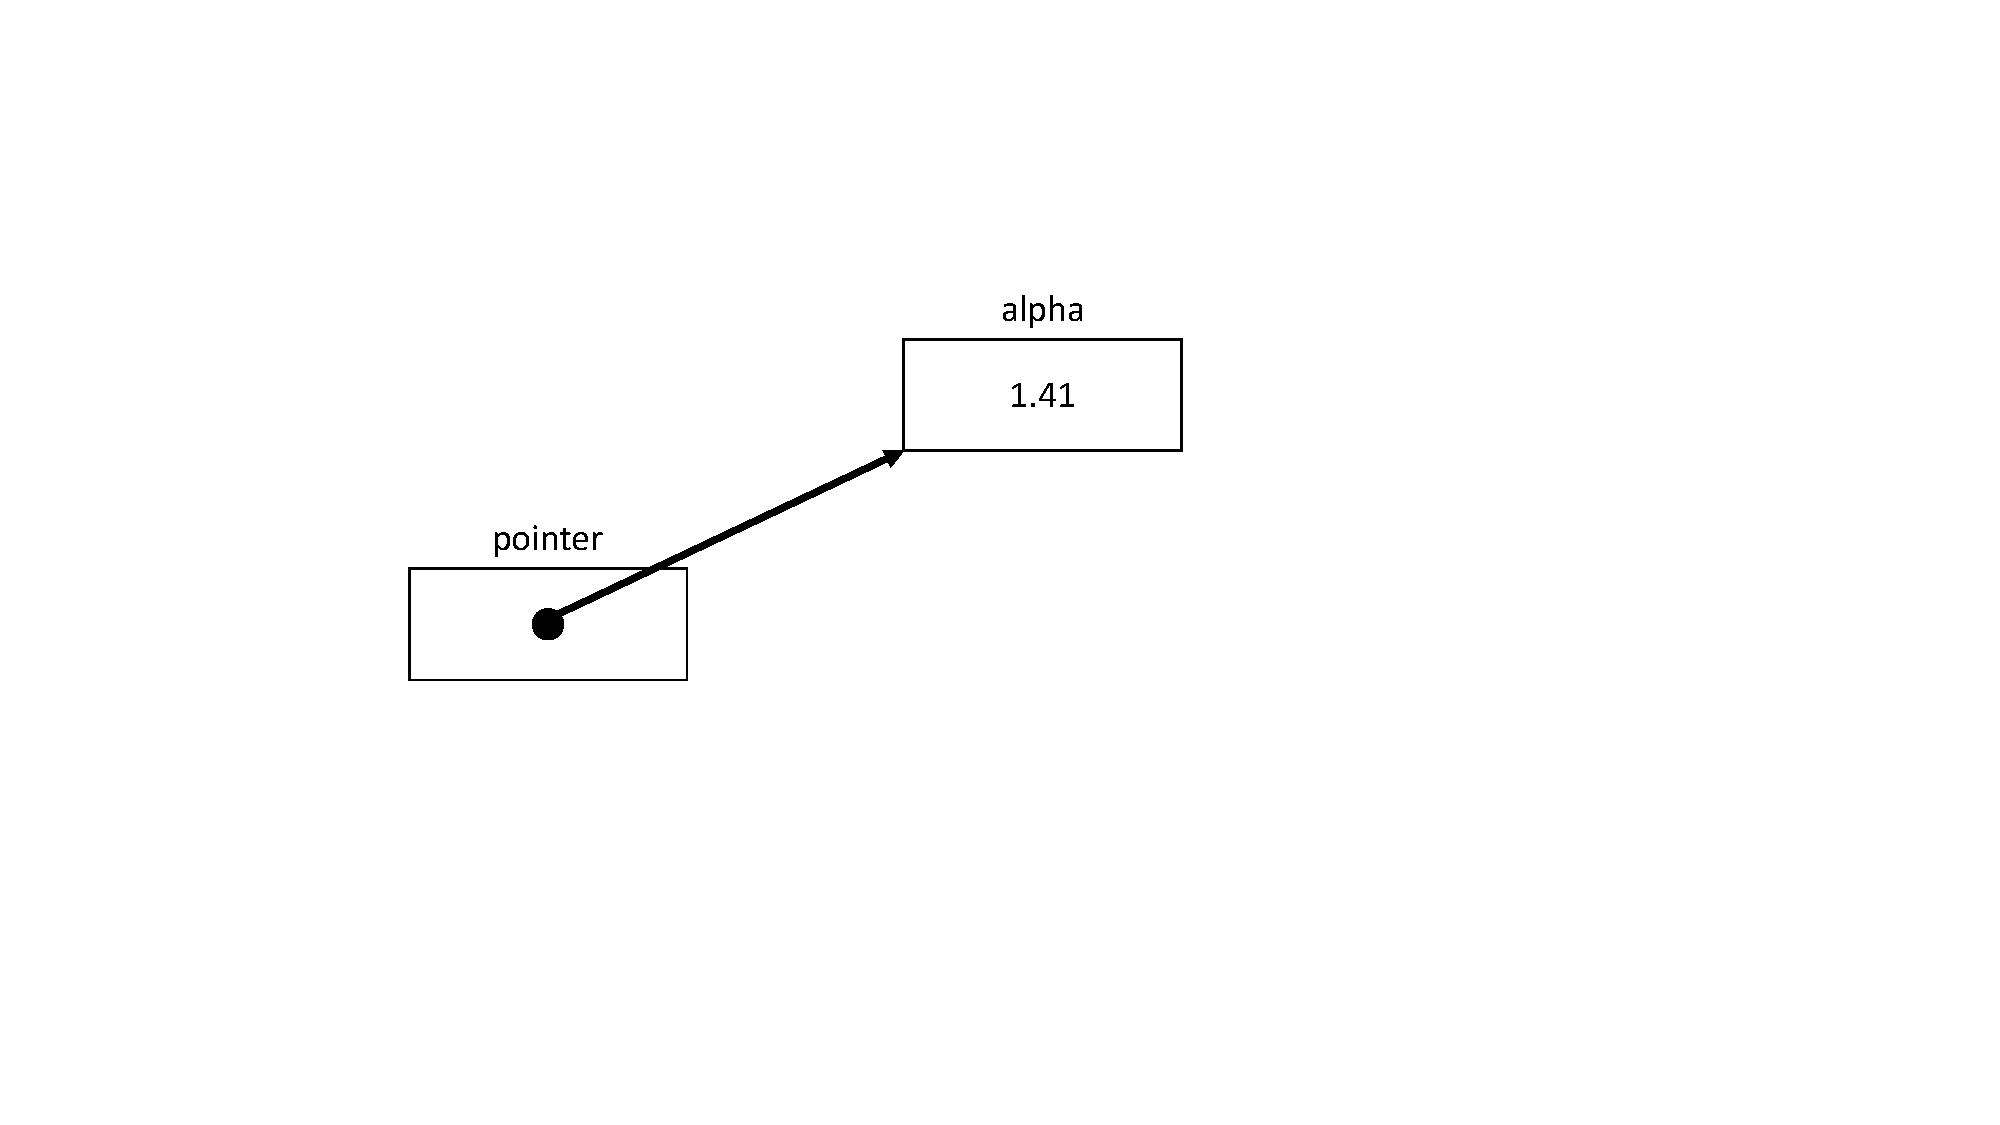
\includegraphics[width=0.4\linewidth]{images/pointer1.pdf}
\end{figure}

\subsubsection{Pointer und Datentyp}
\label{sec:Pointerund Datentyp}
\begin{itemize}
	\item Pointer in C++ sind typisiert (wie in C), sie zeigen auf eine Variable des definierten Typs
	\item Oder anders ausgedrückt:
		\\ Der Speicherbereich, auf den ein bestimmter Pointer zeigt, wird entsprechend des definierten Pointer-Typs interpretiert
	\item Der Speicherbedarf einer Pointervariablen ist unabhängig vom Pointer-Typ. Er ist so gross, dass die maximale Adresse Platz findet
		\\ (z.B. 32 Bits für $2^{32}$ Adressen)
\end{itemize}

\subsubsection{Definition einer Pointervariablen}
\label{sec:Definition einer Pointervariablen}
\noindent
\begin{minipage}{\linewidth}
\begin{lstlisting}
*@// Datentyp des Pointers	Kennzeichnung des Pointers durch '\color{blue}*\color{black}'@*
*@\color{red}Typname\color{blue}* \color{black} pointerName;@*

// Konkrete Beispiele:

int* ptr1;		// ptr1 ist ein Pointer auf int
double* ptr2;	// ptr2 ist ein Pointer auf double
\end{lstlisting}
\end{minipage}
\begin{figure}[h]
	\centering
	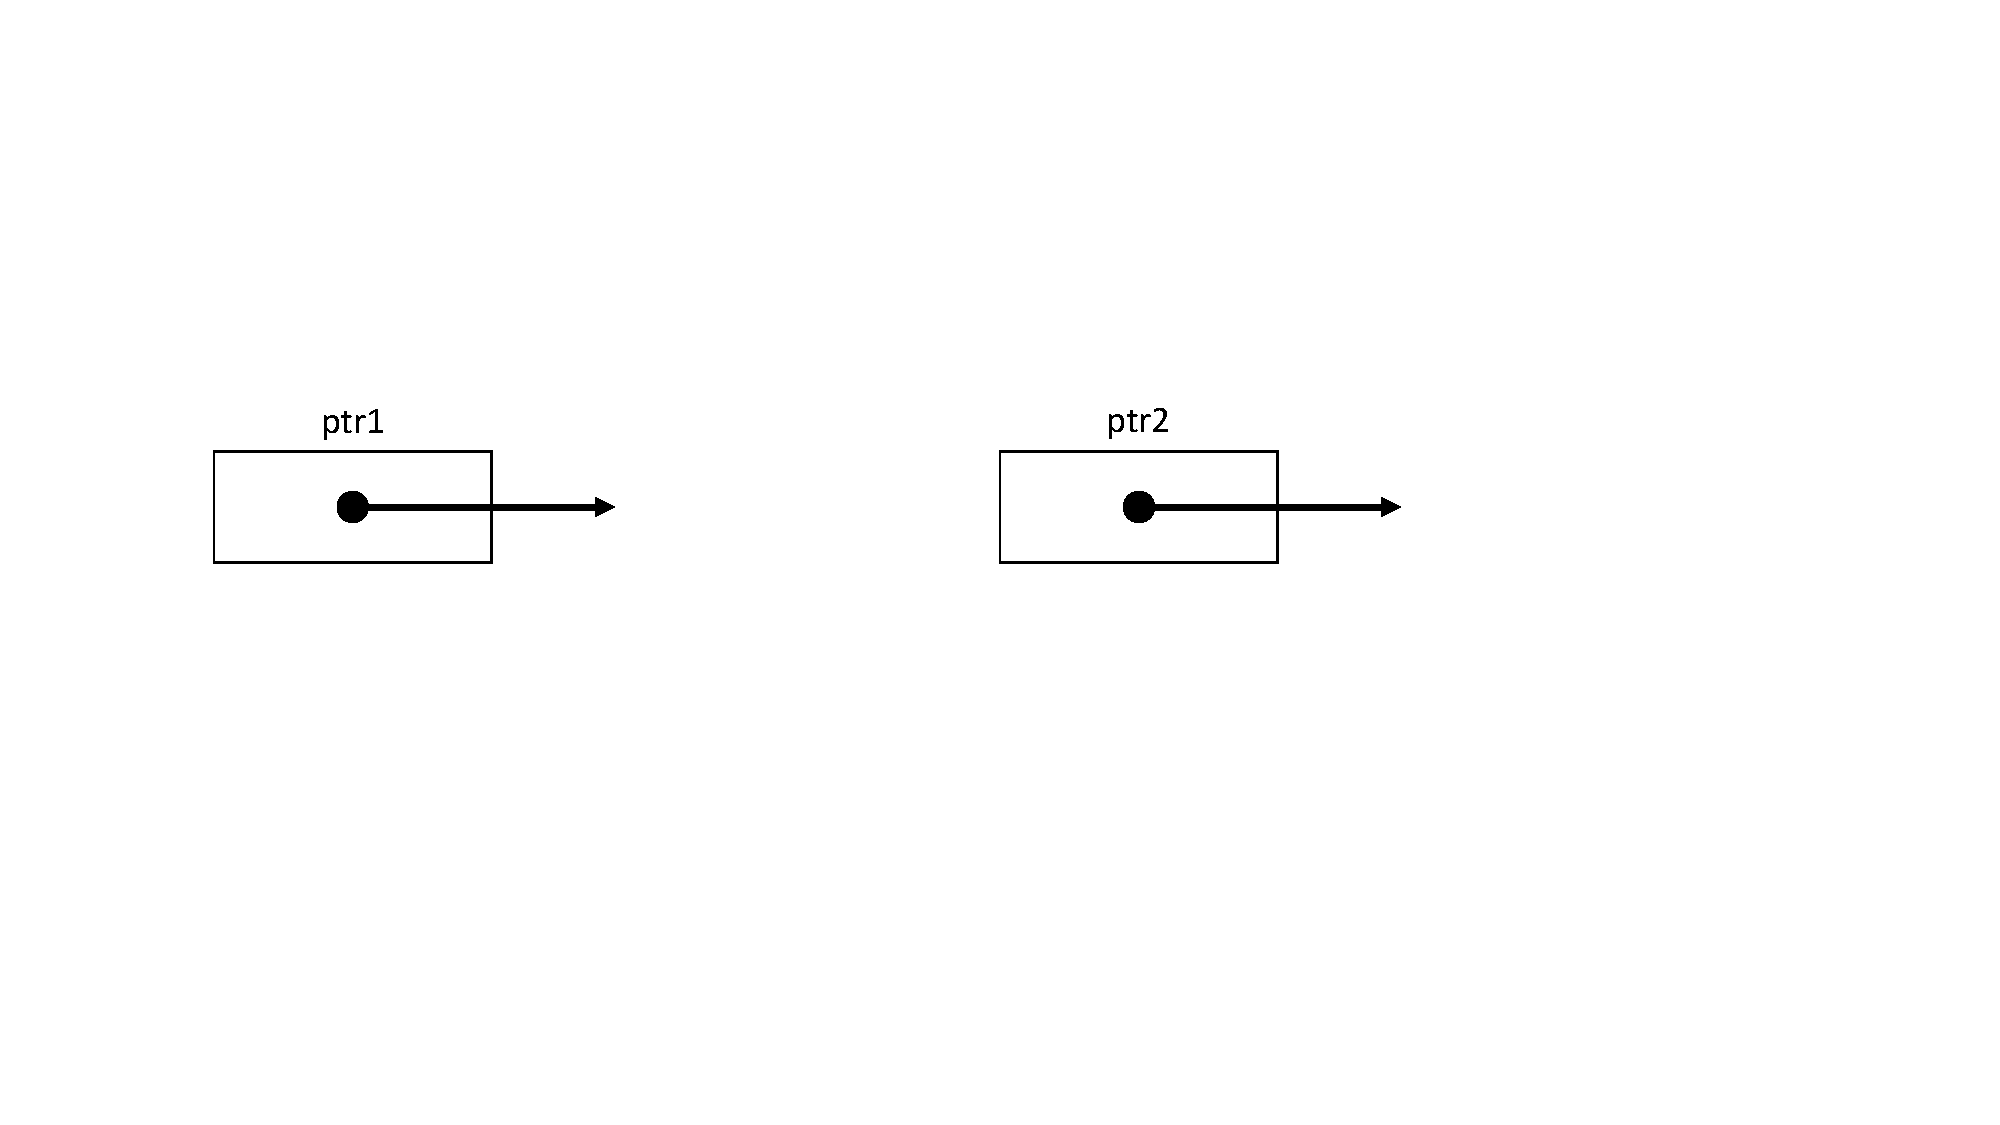
\includegraphics[width=0.5\linewidth]{images/pointer2.pdf}
\end{figure}

\subsubsection{Initialisierung mit Null-Pointer}
\label{sec_Initialisierung mit Null-Pointer}
Mit dem Null-Pointer wird angezeigt, dass der Pointer auf \textbf{kein} Objekt zeigt. Dem Pointer wird ein definierter Nullwert zugewiesen.\\
\\
\begin{hinweis}
Der Pointer zeigt nicht auf die Adresse 0!
\end{hinweis}
\\
\\
\noindent
\begin{minipage}{\linewidth}
\begin{lstlisting}
int* ptr = 0;	// bitte nicht NULL verwenden!
\end{lstlisting}
\end{minipage}
\begin{figure}[h]
	\centering
	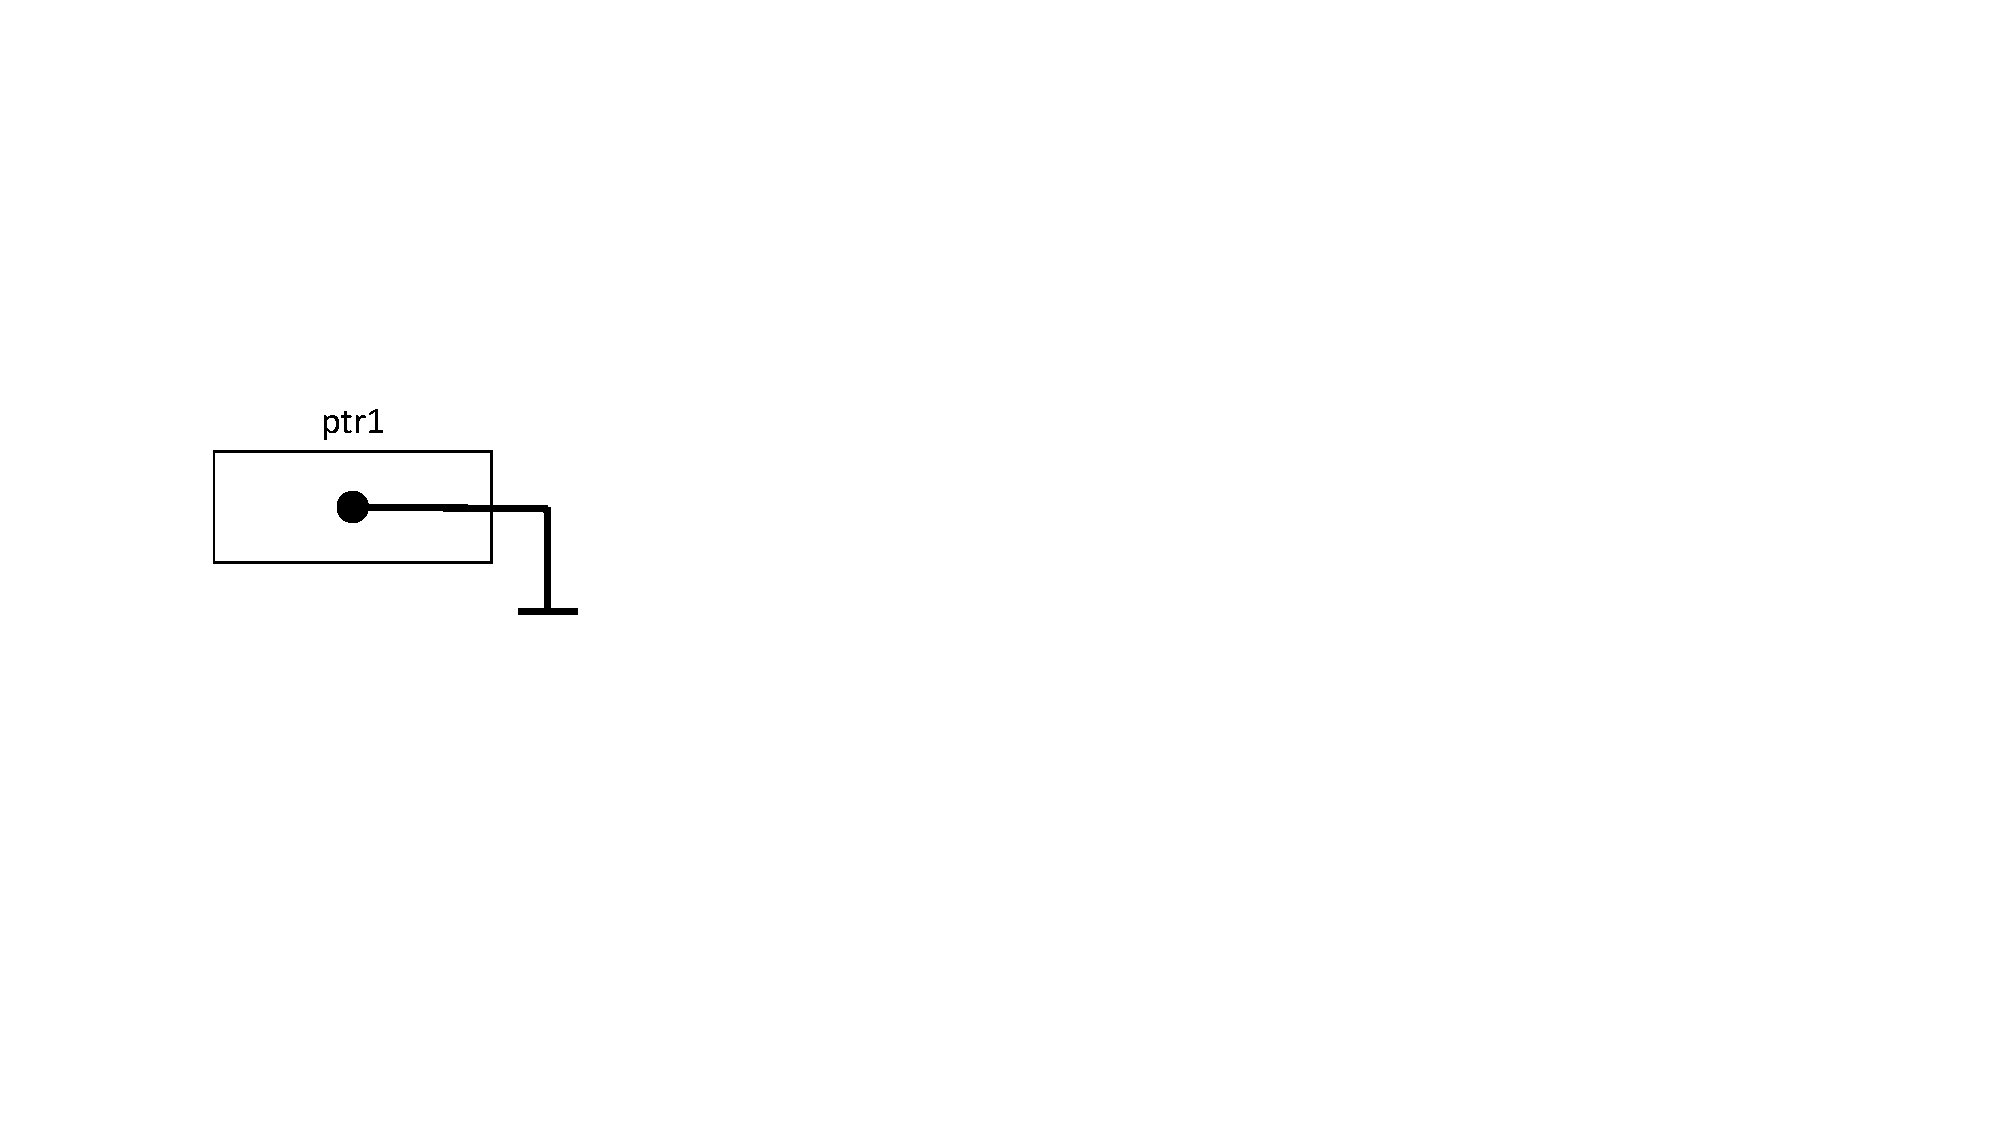
\includegraphics[width=0.2\linewidth]{images/pointer3.pdf}
\end{figure}

\subsubsection{Der Adressoperator \& \textbf{(Referenzierung)}}
\label{sec:Der Adressoperator}
Ist x eine Variable vom Typ Typname, so liefert der Ausdruck \&x einen Pointer auf die Variable x, d.h. er liefert die Adresse der Variablen x.\\
\\
\noindent
\begin{minipage}{\linewidth}
\begin{lstlisting}
int wert;		// Variable wert vom Typ int wird definiert
int* ptr;		// Pointer ptr auf den Typ int wird definiert
			// ptr zeigt auf eine nicht definierte Adresse
		
ptr = &wert;		// ptr zeigt nun auf die Variable wert, d.h. 
			// ptr enthaelt die Adresse der Variablen wert
\end{lstlisting}
\end{minipage}

\subsubsection{Kopieren von Adressen}
\label{sec:Kopieren von Adressen}
\noindent
\begin{minipage}{\linewidth}
\begin{lstlisting}
float alpha;
float* ptr1 = &alpha;
\end{lstlisting}
\end{minipage}
\begin{figure}[h!]
	\centering
	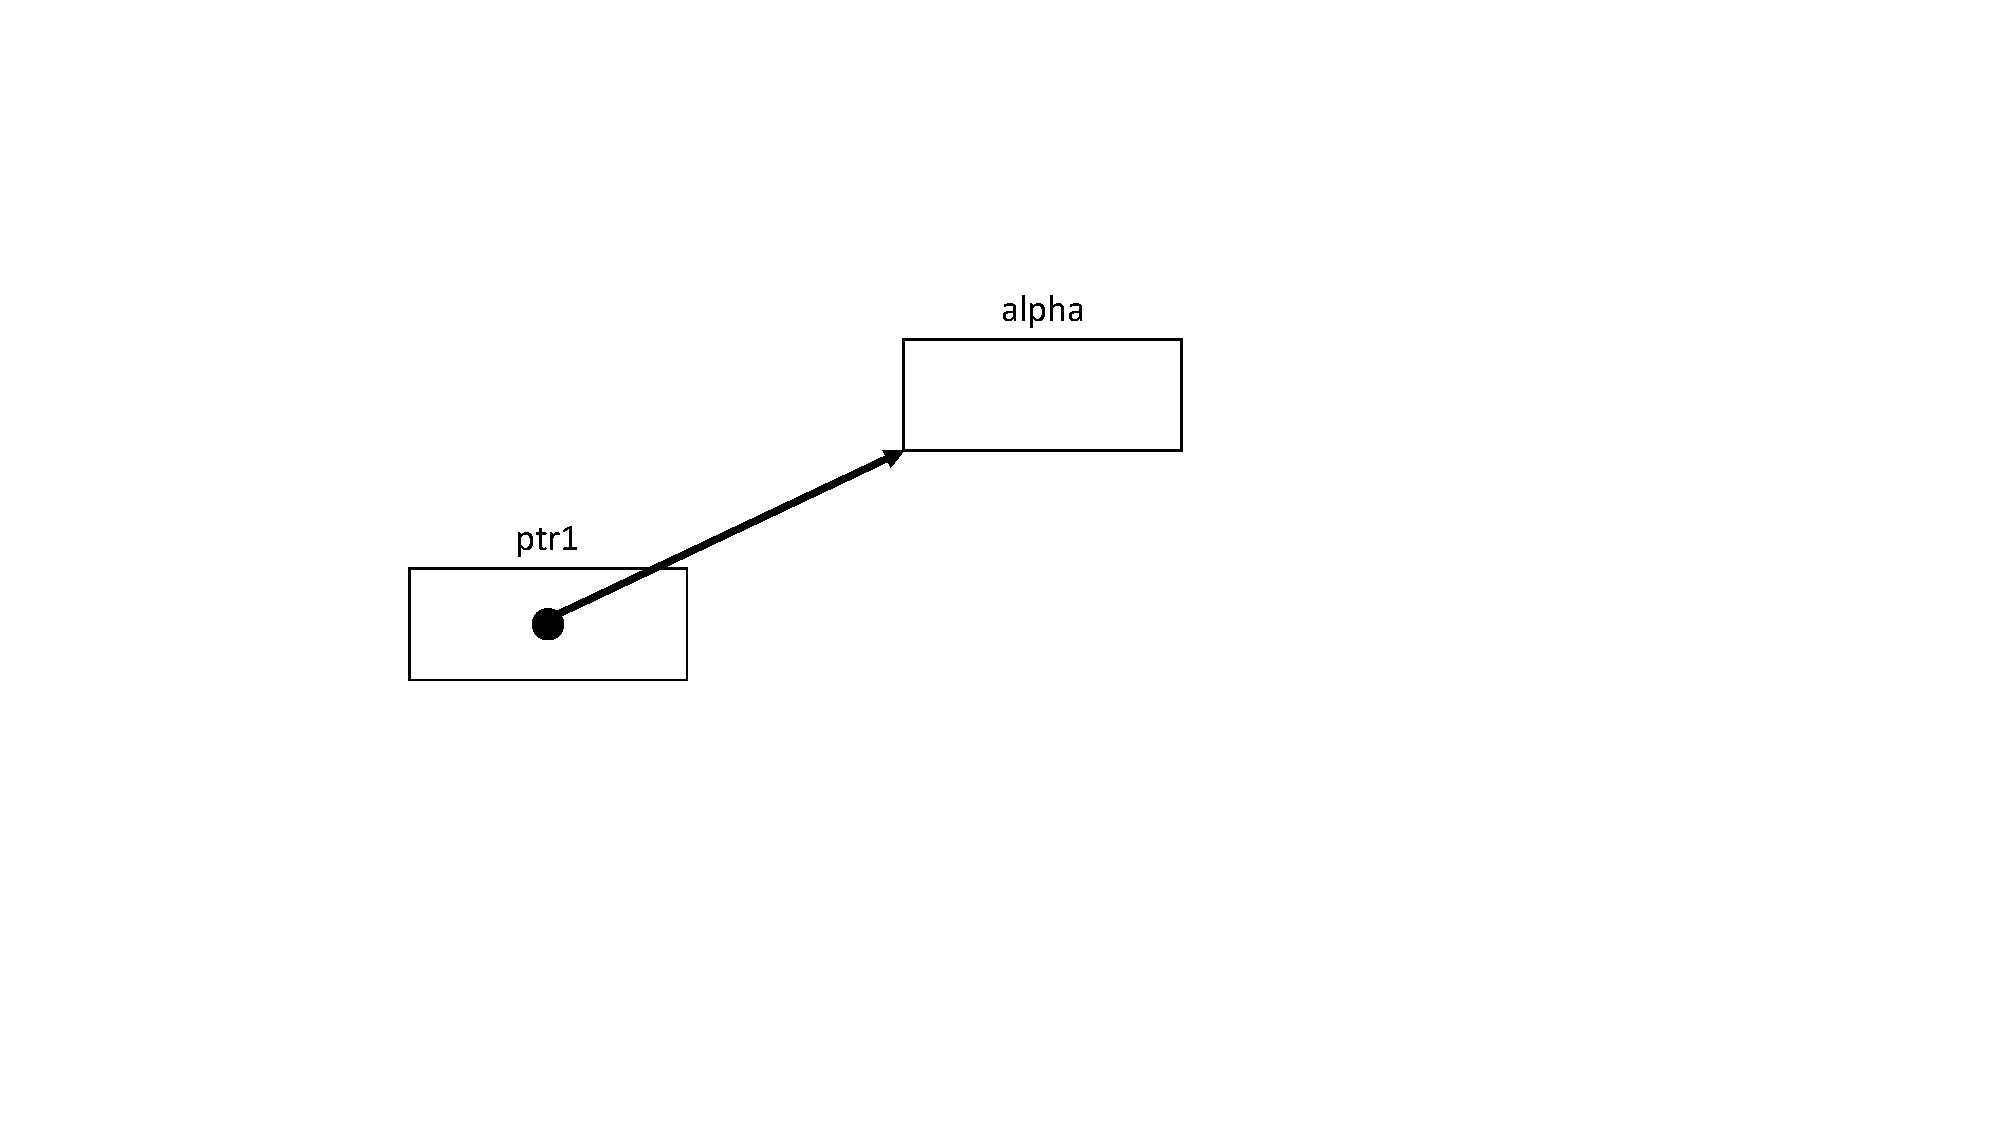
\includegraphics[width=0.4\linewidth]{images/pointer4.pdf}
\end{figure}
\\ \\ \\
\noindent
\begin{minipage}{\linewidth}
\begin{lstlisting}
float* ptr2;
\end{lstlisting}
\end{minipage}
\begin{figure}[h!]
	\centering
	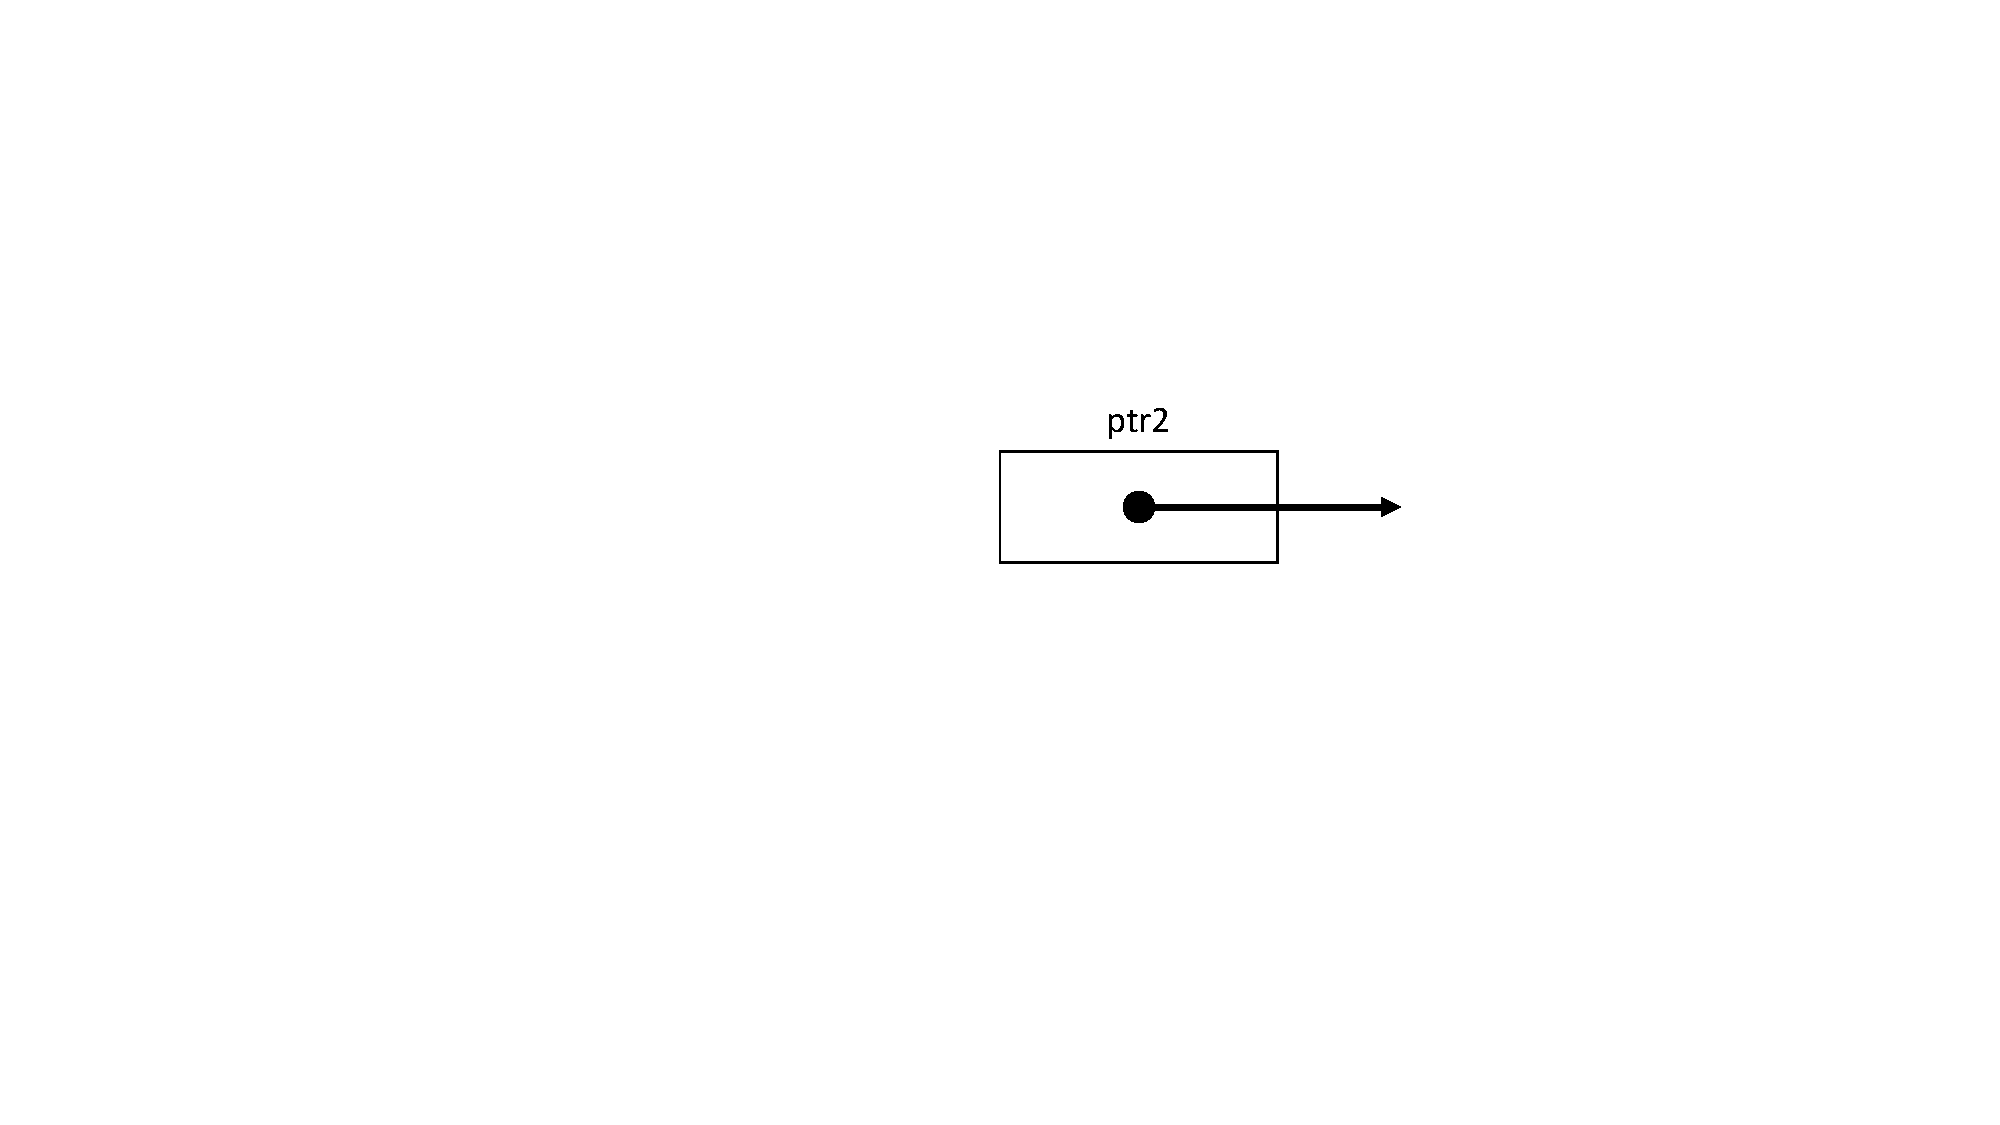
\includegraphics[width=0.2\linewidth]{images/pointer5.pdf}
\end{figure}
\\ \\ \\
\noindent
\begin{minipage}{\linewidth}
\begin{lstlisting}
ptr2 = ptr1;
\end{lstlisting}
\end{minipage}
\begin{figure}[h!]
	\centering
	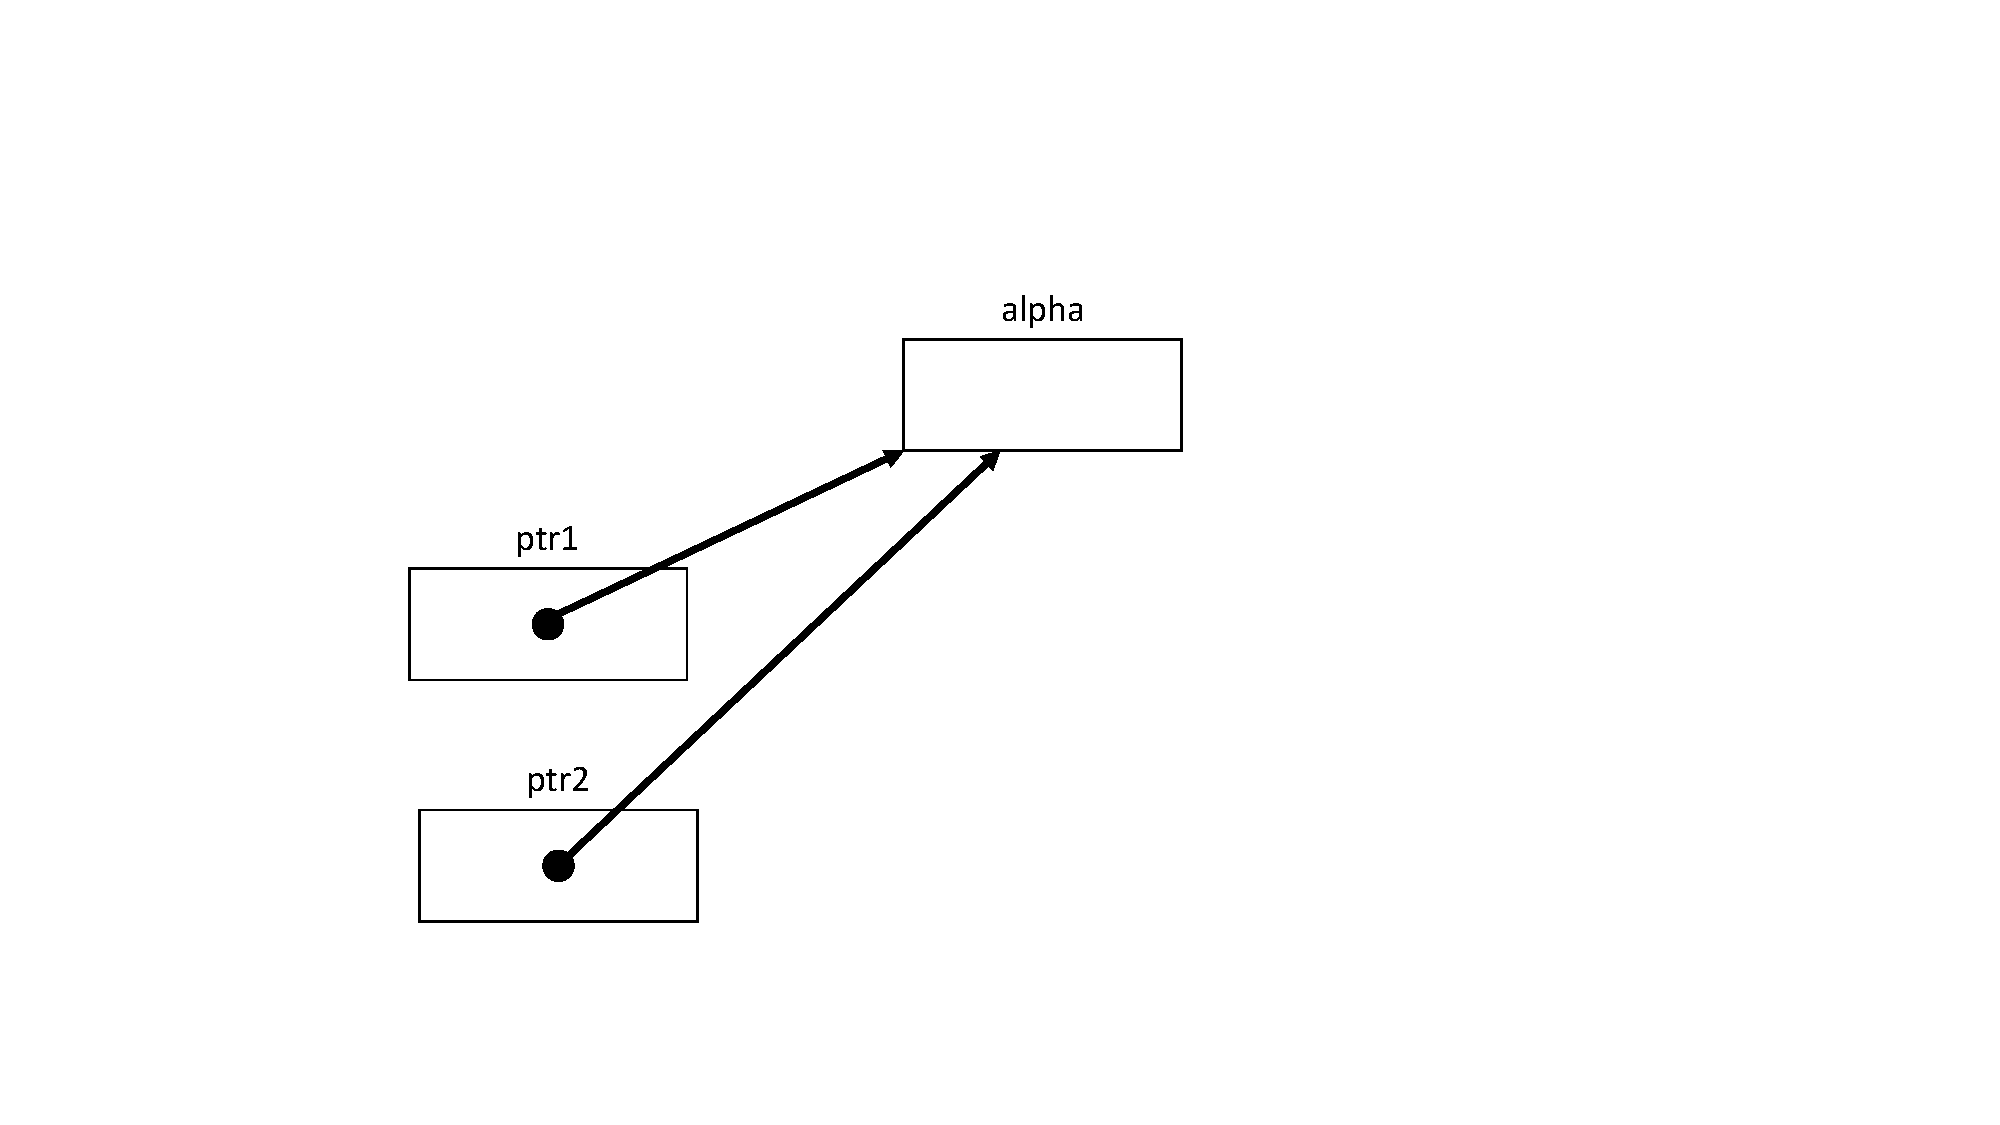
\includegraphics[width=0.4\linewidth]{images/pointer6.pdf}
\end{figure}
\\ \\ \\

\subsubsection{Der Inhaltsoperator * \textbf{(Dereferenzierung)}}
\label{sec:Der Inhaltsoperator}
Ist ptr ein Pointer vom Typ Typname, so liefert der Ausdruck *ptr den Inhalt der Speicherzelle, auf welche ptr zeigt.\\
\\
\noindent
\begin{minipage}{\linewidth}
\begin{lstlisting}
int wert;	// Variable wert vom Typ int wird definiert
int* ptr;	// Pointer ptr auf den Typ int wird definiert
		// ptr zeigt auf eine nicht definierte Adresse
ptr = &wert;	// ptr zeigt nun auf die Variable wert, d.h.
		// ptr enthaelt die Adresse der Variablen wert
*ptr = 23;	// in die Speicherzelle, auf welche ptr zeigt
		// (hier: auf die Variable wert), wird 23 geschrieben.
		// Aequivalent: wert = 23;
\end{lstlisting}
\end{minipage}

\subsubsection{Darstellung in graphischer Pointernotation}
\label{sec:Darstellung in graphischer Pointernotation}
\noindent
\begin{minipage}{\linewidth}
\begin{lstlisting}
int wert;
int* ptr;
ptr = &wert;
\end{lstlisting}
\end{minipage}
\begin{figure}[h]
	\centering
	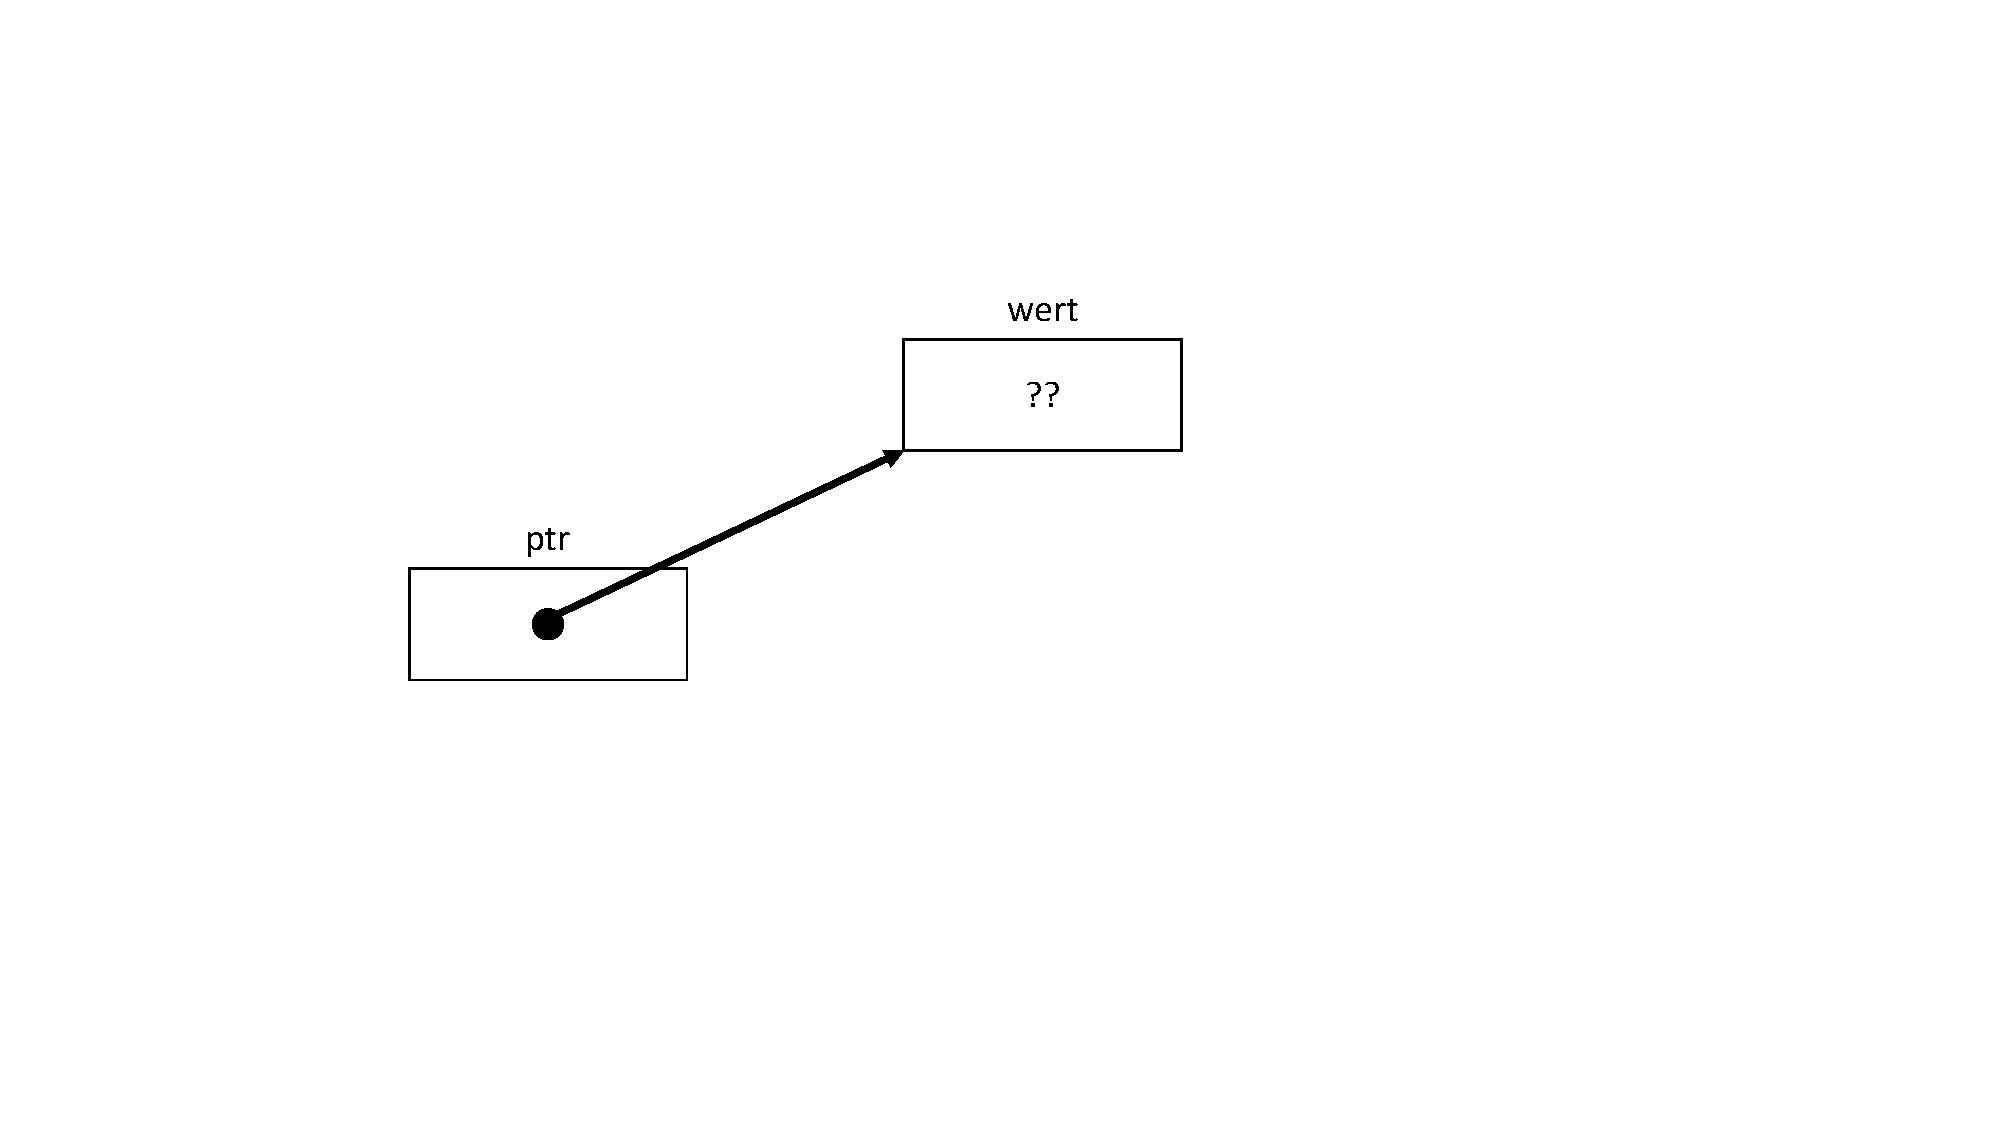
\includegraphics[width=0.4\linewidth]{images/pointer7.pdf}
\end{figure}
\\ \\ \\
\noindent
\begin{minipage}{\linewidth}
\begin{lstlisting}
*ptr = 23;
\end{lstlisting}
\end{minipage}
\begin{figure}[h]
	\centering
	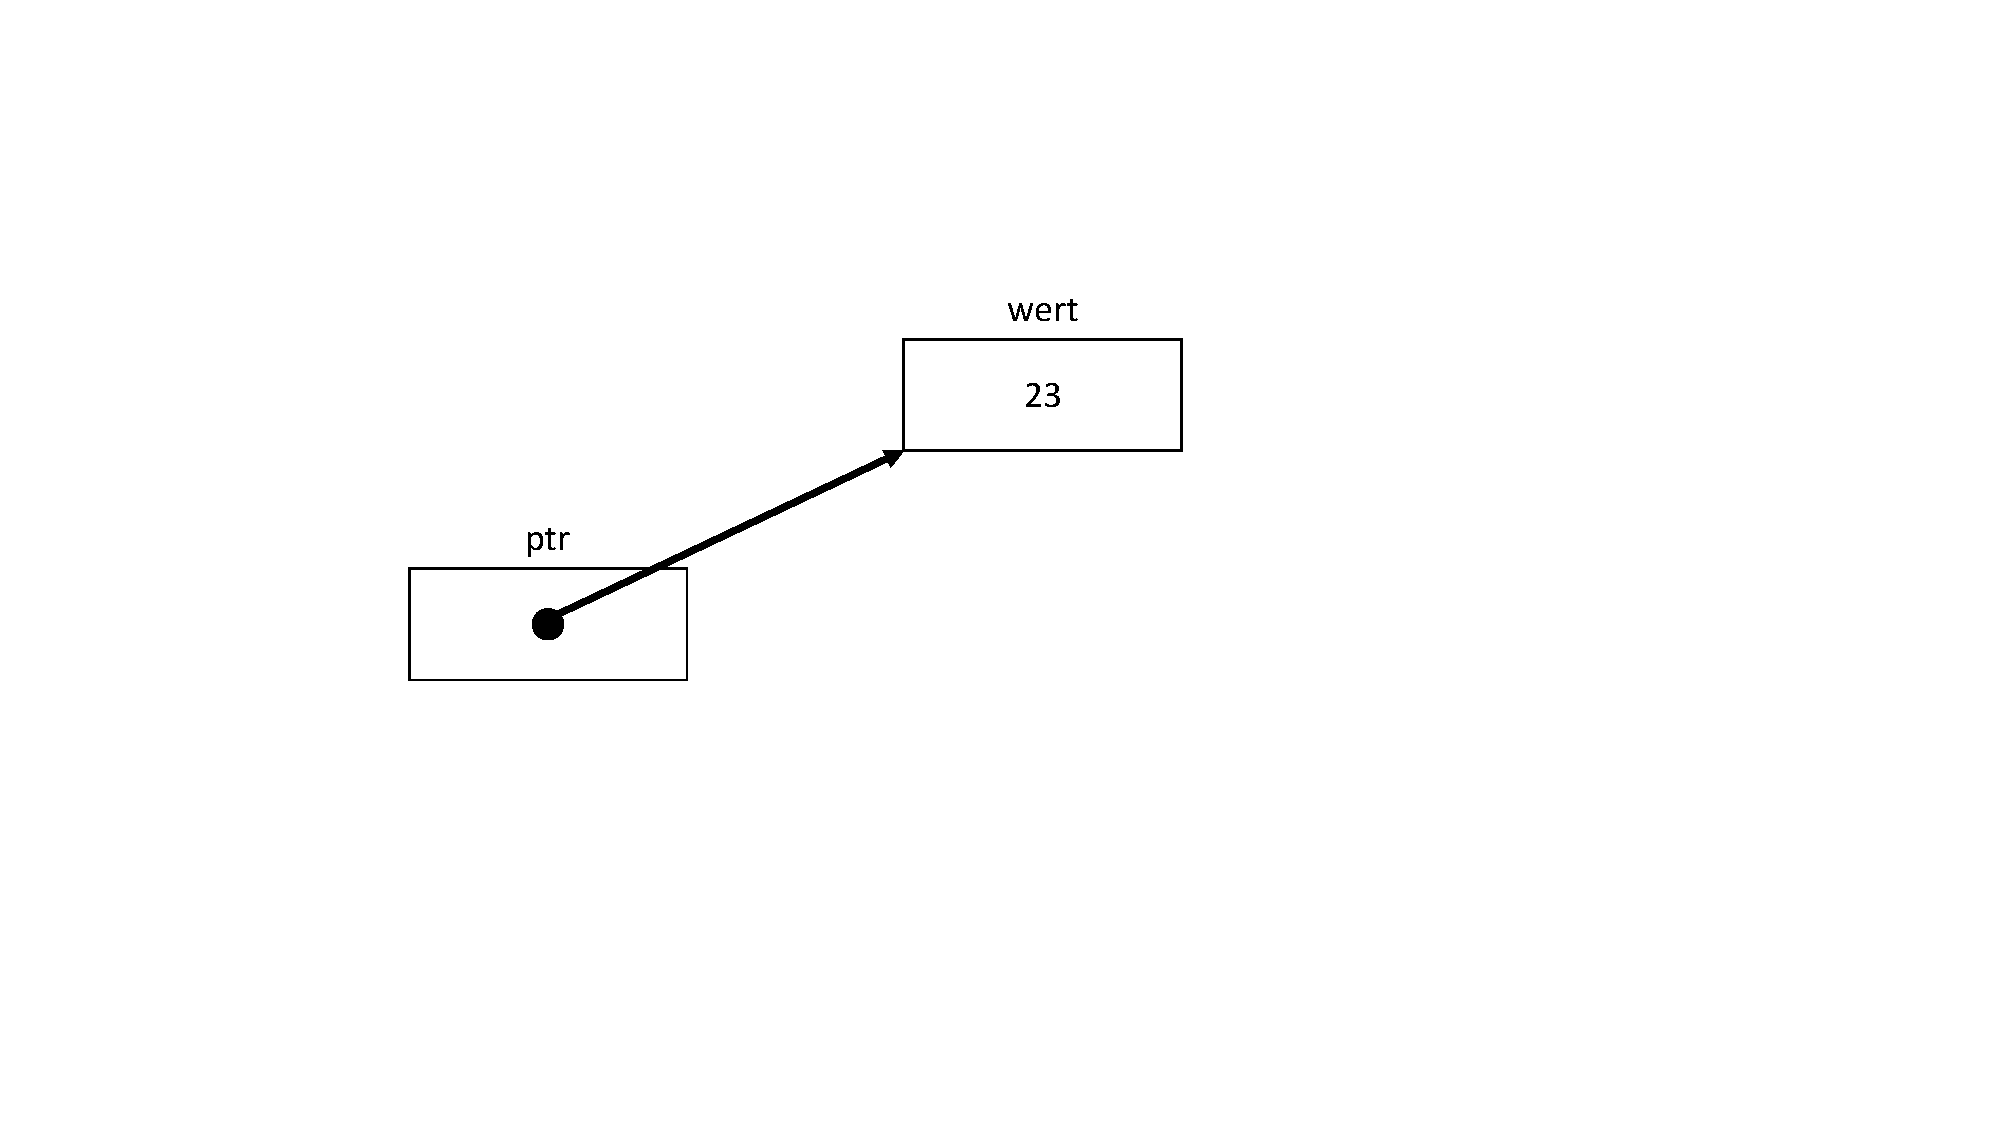
\includegraphics[width=0.4\linewidth]{images/pointer8.pdf}
\end{figure}
\\ \\ \\

\subsubsection{const bei Pointern: Vorsicht}
\label{sec:const bei Pointern: Vorsicht}
\underline{1. Variante: konstanter String}\\
\noindent
\begin{minipage}{\linewidth}
\begin{lstlisting}
char str[] = ''Ein String'';
const char* text = str:
\end{lstlisting}
\end{minipage}
\\
Dies bedeutet nicht, dass der Pointer text konstant ist, sondern dass text auf einen konstanten String zeigt.\\
Von rechts nach links lesen:\\ ''text ist ein Pointer auf eine char-Konstante''\\
\noindent
\begin{minipage}{\linewidth}
\begin{lstlisting}
char ch = text[1];		// erlaubt (==  'i')
text[1] = 's';			*@\color{red}// nicht erlaubt@*
text = ''Ein anderer String'';	// erlaubt
\end{lstlisting}
\end{minipage}
\\ \\ \\ \\
\underline{2. Variante: konstanter Pointer}\\
\noindent
\begin{minipage}{\linewidth}
\begin{lstlisting}
char str[]  = ''Ein String'';
char* const text = strL;
\end{lstlisting}
\end{minipage}
\\
Hier ist nun der Pointer text konstant. Die Position von const ist sehr relevant!\\
Von rechts nach links lesen:\\ ''text ist ein konstanter Pointer auf ein char''\\
\noindent
\begin{minipage}{\linewidth}
\begin{lstlisting}
char ch = test[1];		// erlaubt (== 'i')
text[1] = 's';			// erlaubt
text = ''Ein anderer String'';	*@\color{red}// nicht erlaubt@*
\end{lstlisting}
\end{minipage}
\\ \\ \\ \\
\underline{3. Variante: konstanter Pointer, konstanter String}\\
\noindent
\begin{minipage}{\linewidth}
\begin{lstlisting}
char str[] = ''Ein String'';
const char* const text = str;
\end{lstlisting}
\end{minipage}
\\
Hier ist nun der Pointer text konstant und der Text, wohin er zeigt.\\
Von rechts nach links lesen:\\''text ist ein konstanter Pointer auf eine char-Konstante''\\
\noindent
\begin{minipage}{\linewidth}
\begin{lstlisting}
char ch = text[1];		// erlaubt (== 'i')
text[1] = 's':			*@\color{red}// nicht erlaubt@*
text = ''Ein anderer String'';	*@\color{red}// nicht erlaubt@*
\end{lstlisting}
\end{minipage}
\\ \\ \\ \\
\underline{const bei Pointern in Funktionsköpfen}\\
\noindent
\begin{minipage}{\linewidth}
\begin{lstlisting}
void foo (const int* ptr)
{
	*ptr = 14;		// nicht erlaubt
}
\end{lstlisting}
\end{minipage}
\\
ptr ist ein Pointer auf eine int-Konstante.
\\

\subsubsection{void-Pointer}
\label{sec:void-Pointer}
\begin{itemize}
	\item void-Pointer sind Objekte, die eine gültige Adresse darstellen
	\item einem void-Pointer kann jeder Pointer zugewiesen werden
	\item \Large{ein void-Pointer kann ohne Typecast nur anderen void-Pointern zugewiesen werden (anders als in C)}\normalsize
	\item ein void-Pointer kann nicht dereferenziert werden
\end{itemize}
\begin{hinweis}
in C++ sollten void-Pointer kaum noch angewendet werden
\end{hinweis}
\underline{void-Pointer: Beispiele}\\
\noindent
\begin{minipage}{\linewidth}
\begin{lstlisting}
int a;
int* pi = &a;
void* pv = pi;			*@\color{green}// ok@*
double* pd = pv			*@\color{red}// Error (in C erlaubt)@*
pd = static_cast<double*>pv;	*@\color{green}// ok@*
\end{lstlisting}
\end{minipage}

\subsubsection{Pointer auf Funktionen}
\label{sec:Pointer auf Funktionen}
\begin{itemize}
	\item Jede Funktion befindet sich an einer definierten Adresse im Codespeicher
	\item Diese Adresse kann ebenfalls ermittelt werden
	\item Interessant wäre, dynamisch zur Laufzeit in Abhängigkeit des Programmablaufs eine unterschiedliche Funktion über einen Funktionspointer aufzurufen
\end{itemize}
\begin{hinweis}
In C++ gibt es für viele Situationen bessere Alternativen zu Funktionspointern (Polymorphismus)
\end{hinweis}

\subsubsection{Interruptvektortabelle: Tabelle von Funktionspointern}
\label{sec:Interruptvektortabelle: Tabelle von Funktionspointern}
\centering
\begin{tabularx}{0.25\textwidth}{|X|}
	\hline
	Pointer auf ISR n\\
	\hline
	...\\
	\hline
	...\\
	\hline
	Pointer auf ISR 2\\
	\hline
	Pointer auf ISR 1\\
	\hline
\end{tabularx}
\flushleft
ISR = Interrupt Service Routine

\subsubsection{Umsetzung von Funktionspointern in C/C++}
\label{sec:Umsetzung von Funktionspointern in C/C++}
Der Name der Funktion kann als Adresse auf den ersten Befehl der Funktion verwendet werden (analog Array).

\subsubsection{Beispiel für Funktionspointer}
\label{sec:Beispiel fuer Funktionspointer}
\lstinputlisting{\listings/ftptr.cpp}

% Unterkapitel: Referenzen

\subsection{Referenzen}
\label{secc:Referenzen}

\subsubsection{Was ist eine Referenz?}
\label{sec:Was ist eine Referenz?}
\begin{itemize}
	\item Eine Referenz ist ein Alternativname (Alias) für ein Objekt
	\item Referenzen ähneln Pointern, sind aber nicht dasselbe. Bei einem Pointer wird immer eine Adresse ermittelt, d.h. dieses Datenobjekt muss sich im adressierbaren Bereich befinden. Eine Referenz kann aber auch auf ein Register verweisen. Grundsätzlich sind Referenzen effizienter als Pointer.
	\item Syntaktisch sind Referenzen einfacher als Pointer, da ein expliziter Referenzierungs- und Dereferenzierungsoperator entfällt
	\item Referenzen sind für den Programmierer sicherer anzuwenden als Pointer
	\item In gewissen Fällen braucht es Pointer. Wenn nicht, dann sollen Referenzen bevorzugt werden.
\end{itemize}

\subsubsection{Syntax von Referenzen}
\label{sec:Syntax von Referenzen}
\noindent
\begin{minipage}{\linewidth}
\begin{lstlisting}
int x = 24;
int& r1 = x;	// Definition der Referenz r1

x = 55;	// x == 55, r1 == 5 (dasselbe Objekt)
r1 = 7;	// x == 7, r1 == 7 (dasselbe Objekt)
r1++;	// x == 8, r1 == 8 (dasselbe Objekt)
\end{lstlisting}
\end{minipage}
\begin{hinweis}
Referenzen können nach der Definition nicht ''umgehängt'' werden, d.h. eine Referenz kann und muss nur bei der Definition initialisiert werden und kann nicht später auf etwas anders ''zeigen''.
\end{hinweis}

\subsubsection{Einsatz von Referenzen}
\label{sec:Einsatz von Referenzen}
\begin{itemize}
	\item In folgenden zwei Fällen einsetzen:
	\begin{itemize}
		\item Bei Parameterübergabe (call by reference) anstatt Pointer (entspricht var-Parameter in der Programmiersprache Pascal)
		\item Bei Referenz-Rückgabetyp anstatt Pointertyp, d.h. als Returntyp
	\end{itemize}
	\item\Large Generell:\\Objekte einer Klasse und Strukturvariablen sollen immer by reference übergeben werden (niemals by value)\normalsize
	\item Sonst: zurückhaltend einsetzen
\end{itemize}

\subsubsection{Pointer und Referenzen auf lokale Variablen}
\label{sec:Pointer und Referenzen auf lokale Variablen}
\begin{achtung}
Sie dürfen niemals einen Pointer oder eine Referenz auf eine lokale Variable oder ein lokales Objekt mittels return zurückgeben
\end{achtung}
Grund:\\Nach Beendigung der Funktion sind die lokalen Variablen ungültig.

% Unterkapitel: Zeiger/Referenzen

\subsection{Zeiger und Referenzen als Parameter und Rückgabewerte}
\label{sec:Zeiger und Referenzen als Parameter und Rueckgabewerte}

\subsubsection{Call by Value vs. Call by Reference}
\label{sec:Call by Value vs. Call by Reference}
\begin{itemize}
	\item Parameter, die by value übergeben werden (Wertparameter) werden kopiert, in der Funktion wird mit Kopien gearbeitet.
	\item Bei Referenzparametern (call by reference) wird nur eine Referenz (Alias) des Originals übergeben.
	\item Nur Parameter, welche by reference übergeben werden, könne in der Funktion (bleibend) verändert werden.
\end{itemize}

\subsubsection{3 Beispiele}
\label{sec:3 Beispiele}
\underline{Versuch 1: Call by value}
\noindent
\begin{minipage}{\linewidth}
\begin{lstlisting}
void swap(int a, int b)
{
	int tmp = 1;
	a = b;
	b = tmp;
}

int main()
{
	int x = 4;
	int y = 3;
	swap(x, y);	*@\color{red}// nur Kopien werden vertauscht!\color{black}@*
	return 0;
}
\end{lstlisting}
\end{minipage}
\underline{Versuche 2: Call by reference mit Referenzen}
\noindent
\begin{minipage}{\linewidth}
\begin{lstlisting}
void swap(int& a, int& b)
{
	int tmp = 1;
	a = b;
	b = tmp;
}

int main()
{
	int x = 4;
	int y = 3;
	swap(x, y);	*@\color{green}// OK!\color{black}@*
	return 0;
}
\end{lstlisting}
\end{minipage}
\underline{Versuch 3: Call by reference mit Pointer}
\noindent
\begin{minipage}{\linewidth}
\begin{lstlisting}
void swp(int* a, int* b)
{
	int tmp = *a;
	*a = *b;
	*b = tmp;
}

int main()
{
	int x = 4;
	int y = 3;
	swap(&x, &y);	*@\color{red}// OK, jedoch muehsame Syntax und evtl. ineffizient\color{black}@*
	return 0;
}
\end{lstlisting}
\end{minipage}

\subsubsection{Call by reference: wann einsetzen?}
\label{sec:Call by reference: wann einsetzen?}
\#1: wenn Parameter in der Funktion verändert werden sollen\\
\#2: wenn ''grosse'' Parameter übergeben werden sollen (struct, class)\\
zu \#2: wenn verhindert werden soll, dass der Parameter verändert wird, so kann dieser mit const deklariert werden\\
\noindent
\begin{minipage}{\linewidth}
\begin{lstlisting}
int foo(const BigType& b);
\end{lstlisting}
\end{minipage}
\begin{achtung}
Parameterübergabe und Rückgabe von Objekten by value ist ein Hauptgrund für langsame C++-Programme!
\end{achtung}

\subsubsection{Merke}
\label{sec:Merke}
\begin{achtung}
Variablen einer Struktur und Variablen einer Klasse (Objekte) müssen immer by reference übergeben werden, niemals by value.\\
Read-only Parameter werden zusätzlich mit const spezifiziert.
\end{achtung}
% ENDE


















\clearpage
%!TEX root = main.tex

\part{Arrays, Dynamische Speicherverwaltung}
\label{sec:Arrays, Dynamische Speicherverwaltung}

% Unterabschnitt: Arrays:Vektoren

\section{Arrays}
\label{sec:Arrays}

\subsection{Arrays: Vektoren}
\label{sec:Arrays: Vektoren}
Problemstellung:\\
Sie müssen 10 Messwerte (z.B. Temperaturwerte) vom Typ int speichern.
\noindent
\begin{minipage}{\linewidth}
\begin{lstlisting}
int data1;
int data2;
int data3;
int data4;
int data5;
int data6;
int data7;
int data8;
int data9;
int data10;
\end{lstlisting}
\end{minipage}

Diese Darstellung ist sehr unhandlich.\\
Wie würden sie 1000 Messwerte abspeichern?

\subsection{Der Array (Feld, Vektor)}
\label{sec:Der Array (Feld, Vektor)}
Ein Array bietet eine kompakte Zusammenfassung von mehreren Variablen des gleichen Typs.
\noindent
\begin{minipage}{\linewidth}
\begin{lstlisting}
int data[10];	// ein Array von 10 int-Werten
int data[1000];	// ein Array von 1000 int-Werten
double zahl[5];	// ein Array von 5 double-Werten
\end{lstlisting}
\end{minipage}

\subsubsection{Zugriff auf ein Arrayelement}
\label{sec:Zugriff auf ein Arrayelement}
\begin{hinweis}
Der Zugriff auf ein Element eines Arrays erfolgt über den Array-Index. Ist ein Array mit n Elementen definiert, so ist darauf zu achten, dass in C++ (wie in C) der Index mit 0 beginnt und mit n-1 endet.
\end{hinweis}
\noindent
\begin{minipage}{\linewidth}
\begin{lstlisting}
int alpha[5];	// der Array 'alpha' mit 5 Elementen vom Typ
	// int wird definiert
alpha[0] = 14;	// 1. Element (Index 0) wird auf 14 gesetzt
alpha[4] = 3;	// das letzte Element (Index 4)

alpha[5] = 4;	\color{red}// Bereichsueberschreitung (geht in C++!)\color{black}
\end{lstlisting}
\end{minipage}

% Unterabschnitt: Arrays und Pointer

\subsection{Arrays und Pointer}
\label{sec:Arrays und Pointer}

\subsubsection{Pro Memoria: Eindimensionales Array (Vektor)}
\label{sec:Pro Memoria: Eindimensionales Array (Vektor)}
\noindent
\begin{minipage}{\linewidth}
\begin{lstlisting}
int alpha[5];
int* ptr;
ptr = &alpha[2];
*ptr = 3452;
\end{lstlisting}
\end{minipage}
\begin{figure}[h]
	\centering
	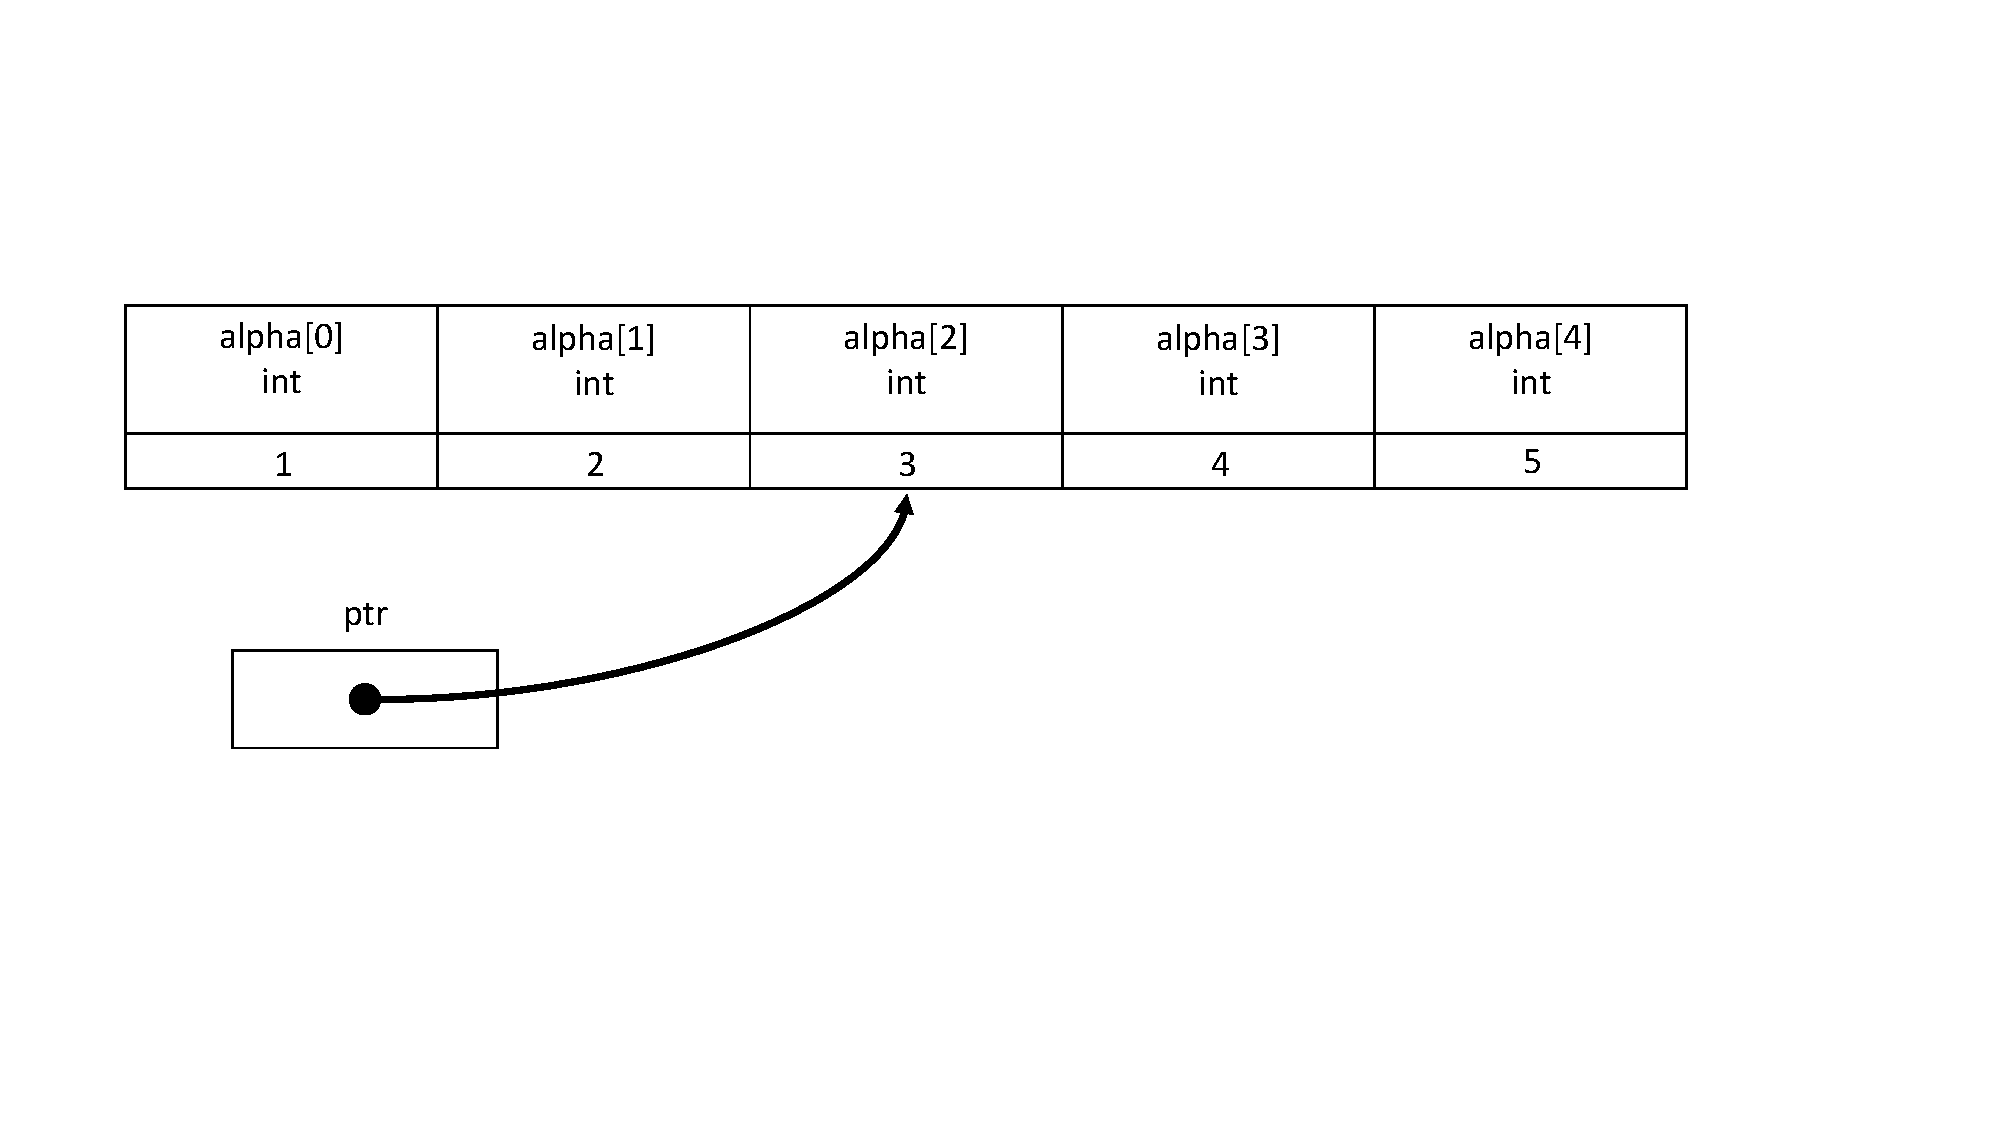
\includegraphics[width=\linewidth]{images/pointer9.pdf}
\end{figure}

\subsection{Äquivalenz von Array- und Pointernotation}
\label{sec:Aequivalenz von Array- und Pointernotation}
Der Name des Array kann als konstante Adresse des ersten (Index 0) Elementes des Arrays betrachtet werden.\\
\vspace{5mm}
\begin{figure}[h]
	\centering
	%!TEX root = main.tex

\begin{tikzpicture}
	\node[draw, fit={(0,3.5) (2.5,4.5)}, inner sep=0pt, label=center:alpha{[0]}] (A) {};	% upper rectangles
	\node[draw, fit={(2.5,3.5) (5,4.5)}, inner sep=0pt, label=center:alpha{[1]}] (B) {};
	\node[draw, fit={(5,3.5) (7.5,4.5)}, inner sep=0pt, label=center:alpha{[2]}] (C) {};
	\node[draw, fit={(7.5,3.5) (10,4.5)}, inner sep=0pt, label=center:alpha{[3]}] (D) {};
	\node[draw, fit={(10,3.5) (12.5,4.5)}, inner sep=0pt, label=center:alpha{[4]}] (E) {};

	\draw[-Latex] (-.5,3) node[below] {$alpha$}  -- (A);						% pointers
	\draw[-Latex] (4.5,3) node[below] {$\&alpha[2]$} -- (C);
	
	\node[draw, fit={(7.5,1.625) (12.5,2.825)}, fill=gray!50, inner sep=0pt, label=center:alpha{[i]}{==}*(alpha + i)] () {};	% textbox
	
	\node[draw, fit={(0,0) (2.5,1)}, inner sep=0pt, label=center:*alpha] (F) {};	% lower rectangles
	\node[draw, fit={(2.5,0) (5,1)}, inner sep=0pt, label=center:*(alpha+1)] (G) {};
	\node[draw, fit={(5,0) (7.5,1)}, inner sep=0pt, label=center:*(alpha+2)] (H) {};
	\node[draw, fit={(7.5,0) (10,1)}, inner sep=0pt, label=center:*(alpha+3)] (I) {};
	\node[draw, fit={(10,0) (12.5,1)}, inner sep=0pt, label=center:*(alpha+4)] (J) {};
	
	\draw[-Latex] (-.5,1.5) node[above] {$alpha$} -- (F);
\end{tikzpicture}
\end{figure}

\subsection{Vergleichen von Arrays}
\label{sec:Vergleichen von Arrays}
\begin{itemize}
	\item\color{red}In C++ gibt es keinen Operator ==, der zwei Arrays miteinander vergleicht\color{black}
	\item Arrayvergleiche müssen explizit Element um Element durchgeführt werden
	\item oder: der Inhalt der beiden Speicherbereiche wird mit Hilfe der Funktion memcmp() byteweise verglichen
	\item Beispiel:\\Seien arr1 und arr2 zwei Arrays\\Der Vergleich arr1 == arr2 prüft, ob die Anfangsadressen der beiden Arrays identisch sind (wird kaum der Fall sein), nicht aber, ob deren Inhalte identisch sind.
\end{itemize}
	
\subsection{Arrayname ist ein nicht modifizierbarer L-Wert}
\label{sec:Arrayname ist ein nicht modifizierbarer L-Wert}
\begin{itemize}
	\item Der Arrayname ist die konstante Adresse des ersten Elementes des Arrays und kann nicht verändert werden
	\item Auf den Arraynamen können nur die beiden Operatoren sizeof und \& angewandt werden
	\item Der Arrayname (z.B. arr), als auch der Adressoperator angewandt auf den Arraynamen (\&arr) ergeben einen konstanten Pointer auf das erste Element des Arrays, der Typ ist jedoch verschieden
	\item Einem Arraynamen kann kein Wert zugewiesen werden (einer Pointervariablen schon)
\end{itemize}

\subsection{Automatische Initialisierung von Arrays}
\label{sec:Automatische Initialisierung von Arrays}
\begin{itemize}
	\item Globale Arrays werden automatisch mit 0 initialisiert
	\begin{itemize}
		\item globale Arrays sollten aber nur ausnahmsweise verwendet werden
	\end{itemize}
	\item Lokale Arrays werden nicht automatisch initialisiert
	\begin{itemize}
		\item der Inhalt eines lokalen Arrays ist bei der Definition undefiniert
	\end{itemize}
\end{itemize}

\subsection{Explizite Initialisierung von Arrays}
\label{sec:Explizite Initialisierung von Arrays}
\begin{itemize}
	\item Bei der Definition eines Arrays kann ein Array explizit (''manuell'') initialisiert werden
	\item Der Definition folgt ein Zuweisungsoperator und eine Liste von Initialisierungswerten
	\item Die Liste ist mit geschweiften Klammer begrenzt
	\item Als Werte können nur Konstanten oder Ausdrücke mit Konstanten angegeben werden, \color{red}Variablen sind nicht möglich\color{black}
	\item Die Werte werden mit Kommata getrennt
	\item Nach der Initialisierung können die Elemente nur noch einzeln geändert werden
\end{itemize}

\subsubsection{Beispiel}
\label{sec:ecplizites Array Beispiel}
\noindent
\begin{minipage}{\linewidth}
\begin{lstlisting}
in alpha[3] = {1, 2*5, 3};
\end{lstlisting}
\end{minipage}
ist ''äquivalent'' zu:
\noindent
\begin{minipage}{\linewidth}
\begin{lstlisting}
int alpha [3];

alpha[0] = 1;
alpha[1] = 2*5;
alpha[2] = 3;
\end{lstlisting}
\end{minipage}

\subsubsection{Goodies für die explizite Initialisierung}
\label{sec:Goodies fuer die explizite Initialisierung}
\begin{itemize}
	\item Werden bei der Initialisierung weniger Werte angegeben als der Array Elemente hat, so werden die restlichen Elemente mit 0 belegt.\\
	\noindent
	\begin{minipage}{\linewidth}
	\begin{lstlisting}
	int alpha[200] = {3, 105, 17};
	// alpha[3] bis alpha[199] werden gleich 0 gesetzt
	\end{lstlisting}
	\end{minipage}
	\item wird bei der Definition keine Arraygrösse angegeben, so zählt der Compiler die Anzahl Elemente automatisch (offenes Array ohne Längenangabe)
	\noindent
	\begin{minipage}{\linewidth}
	\begin{lstlisting}
	int alpha[] = {1, 2, 3, 4};
	\end{lstlisting}
	\end{minipage}
\end{itemize}

% Unterabschnitt: Mehrdimensionale Arrays

\subsection{Mehrdimensionale Arrays}
\label{sec:Mehrdimensionale Arrays}
\noindent
\begin{minipage}{\linewidth}
\begin{lstlisting}
int alpha[3][4];
\end{lstlisting}
\end{minipage}
\textbf{Matrix}\\
Kann betrachtet werden als Vektor alpha[0] bis alpha[2], wobei jedes Vektorelement wiederum einen Vektor mit 4 Elementen enthält\\
\vspace{5mm}
\begin{figure}[h]
	\centering
	%!TEX root = main.tex

\begin{tikzpicture}
	\node[draw, fit={(-7,0) (-5,1)}, inner sep=0pt, label=center:alpha{[2]}] (A) {};	% row
	\node[draw, fit={(-7,1) (-5,2)}, inner sep=0pt, label=center:alpha{[1]}] (B) {};
	\node[draw, fit={(-7,2) (-5,3)}, inner sep=0pt, label=center:alpha{[0]}] (C) {};	

	\node[draw, fit={(0,0) (1.5,1)}, inner sep=0pt, label=center:{[2][0]}] (AA) {};	% matrix
	\node[draw, fit={(1.5,0) (3,1)}, inner sep=0pt, label=center:{[2][1]}] (AB) {};
	\node[draw, fit={(3,0) (4.5,1)}, inner sep=0pt, label=center:{[2][2]}] (AC) {};
	\node[draw, fit={(4.5,0) (6,1)}, inner sep=0pt, label=center:{[2][3]}] (AD) {};
	\node[draw, fit={(0,1) (1.5,2)}, inner sep=0pt, label=center:{[1][0]}] (BA) {};
	\node[draw, fit={(1.5,1) (3,2)}, inner sep=0pt, label=center:{[1][1]}] (BB) {};
	\node[draw, fit={(3,1) (4.5,2)}, inner sep=0pt, label=center:{[1][2]}] (BC) {};
	\node[draw, fit={(4.5,1) (6,2)}, inner sep=0pt, label=center:{[1][3]}] (BD) {};
	\node[draw, fit={(0,2) (1.5,3)}, inner sep=0pt, label=center:{[0][0]}] (CA) {};
	\node[draw, fit={(1.5,2) (3,3)}, inner sep=0pt, label=center:{[0][1]}] (CB) {};	
	\node[draw, fit={(3,2) (4.5,3)}, inner sep=0pt, label=center:{[0][2]}] (CC) {};
	\node[draw, fit={(4.5,2) (6,3)}, inner sep=0pt, label=center:{[0][3]}] (CD) {};
	
	\draw[-Latex] (-1,2.5) node[left] {$Zeilenindex$}  -- (.4,2.5);						% pointers
	\draw[-Latex] (1,4) node[above] {$Spaltenindex$} -- (1,2.75);
\end{tikzpicture}
\end{figure}

\subsubsection{Initialisierung eines mehrdimensionalen Arrays}
\label{sec:Initialisierung eines mehrdimensionalen Arrays}
\noindent
\begin{minipage}{\linewidth}
\begin{lstlisting}
int alpha[3][4] = {
	{1, 3, 5, 7},
	{2, 4, 6, 8},
	{3, 5, 7, 9}
	};
// aequivalent dazu ist die folgende Definition:
int alpha[3][4] = {1, 3, 5, 7, 2, 4, 6, 8, 3, 5, 7, 9};
\end{lstlisting}
\end{minipage}
\\
\centering
\begin{tabularx}{0.25\textwidth}{|X|X|X|X|}
	\hline
	1 & 3 & 5 & 7\\
	\hline
	2 & 4 & 6 & 8\\
	\hline
	3 & 5 & 7 & 9\\
	\hline
\end{tabularx}
\flushleft
\begin{hinweis}
	Das erste Element kann offen sein, das zweite muss angegeben werden.
\end{hinweis}


% Unterabschnitt: Übergabe von Arrays und Zeichenketten

\section{Übergabe von Arrays und Zeichenketten}
\label{sec:Uebergabe von Arrays und Zeichenketten}
\begin{itemize}
	\item Bei der Übergabe eines Arrays an eine Funktion wird als Argument der Arrayname übergeben. (i.e. Pointer auf erstes Element des Arrays)
	\item Der formale Parameter für die Übergabe eines eindimensionalen Arrays kann ein offenes Array sein oder ein Pointer auf den Komponententyp des Arrays.
	\item Zeichenketten sind char-Arrays und werden deshalb gemäss der oben erwähnten Punkte gehandhabt.
\end{itemize}

\subsection{Beispiel: Array (Vektor) als Parameter}
\label{sec:Beispiel: Array (Vektor) als Parameter}
\noindent
\begin{minipage}{\linewidth}
\begin{lstlisting}
enum {groesse = 3};

void init(int* alpha, int size);	// int* alpha == Pointer auf Arrayelement
void ausgabe(int alpha[], int size);	// int alpha[] == offener Array

int main()
{
	int arr[groesse];
	init(arr, sizeof(arr)/sizeof(arr[0]));	// Argument ist Name des Arrays
	ausgabe(arr, sizeof(arr)/sizeof(arr[0]));// Argument ist Name des Arrays
	return 0;
}
\end{lstlisting}
\end{minipage}

\subsection{Übergabe einer Matrix mittels offenem Array}
\label{sec:Uebergabe einer Matrix mittels offenem Array}
\noindent
\begin{minipage}{\linewidth}
\begin{lstlisting}
void printMat(const double* const mat[],	// Matrix
	int m,					// Anzahl Zeilen
	int n);					// Anzahl Spalten
\end{lstlisting}
\end{minipage}
\begin{itemize}
	\item Der Aufruf erfolgt mit \hspace{5mm}printMat(matA, rows, cols); // bevorzugt\\
		oder	\hspace{3.4cm} printMat(\&matA[0], rows, cols);\\
		oder \hspace{3.4cm} printMat(\&(\&matA[0])[0], rows, cols);
	\item matA \hspace{1cm} ist vom Typ double**\\
		matA[0] \hspace{6mm} ist vom Typ double*\\
		matA[0][0] \hspace{2mm} ist vom Typ double
\end{itemize}

\subsection{Zeichenketten (Strings)}
\label{sec:Zeichenketten (Strings)}
\begin{itemize}
	\item Strings sind char-Arrays, abgeschlossen mit dem Zeichen `\textbackslash0`, bzw. 0 (alles analog C)
\end{itemize}

\section{Dynamische Speicherverwaltung}
\label{sec:Dynamische Speicherverwaltung}

\subsection{Pro Memoria: Variablen}
\label{sec:Pro Memoria: Variablen}
\begin{itemize}
	\item Variablen erleichtern u.a. den Zugriff auf Speicherstellen
	\begin{itemize}
		\item statt über eine Adresse kann auf die Speicherstelle mit Hilfe des Variablennamens zugegriffen werden
	\end{itemize}
	\item Die Variablen müssen zur Entwicklungszeit im Code definiert werden
	\begin{itemize}
		\item zur Laufzeit können keine neuen Variablen erzeugt werden
		\item der gesamte Speicherbedarf muss zur Entwicklungszeit statisch mittels Variablen festgelegt werden
		\item wie gross wähle ich z.B. einen Array, welcher Messwerte enthält?
		\item weiss ich zur Entwicklungszeit bereits die zahl der Messwerte?
	\end{itemize}
	\item Der Speicher einer Variablen wird automatisch freigegeben, sobald die Variable nicht mehr gültig ist
\end{itemize}

\subsection{Dynamische Speicherverwaltung}
\label{sec:Dynamische Speicherverwaltung 2}
\begin{itemize}
	\item Speicher kann zur Laufzeit (dynamisch) vom System angefordert werden
	\begin{itemize}
		\item Operator: new (in C: Funktion malloc())
	\end{itemize}
	\item Dynamisch allozierter Speicher muss wieder explizit freigegeben werden
	\begin{itemize}
		\item Operator: delete (in C: Funktion free())
	\end{itemize}
	\item Dynamischer Speicher wird nicht auf dem Stack angelegt, sondern auf dem \textbf{Heap}
	\item Auf dynamischen Speicher kann \textbf{nur über Pointer} zugegriffen werden
\end{itemize}
\begin{achtung}
Zugriff auf dynamischen Speicher nie verlieren!
\end{achtung}

\subsection{Syntax}
\label{sec:Dynamische Speicherverwaltung: Syntax}
\noindent
\begin{minipage}{\linewidth}
\begin{lstlisting}
int* pint = new int;	// Speicher fuer int alloziert
char* pCh1 = new char;	// Speicher fuer char alloziert
char* pCh2 = new char;	// Speicher fuer char alloziert

*pInt = 23;
std::cin >> *pCh1;
pCh2 = pCh1;
*@\color{red}// pCh2 zeigt nun auch auf die Speicherstelle, auf welche pCh1 zeigt.@*
*@\color{red}// Damit geht aber der Zugriff auf die Speicherstelle verloren, auf die pCh2 gezeigt hat@*
*@\color{red}\hspace{5mm}(Memory Leak!)@*

delete pInt;	// Speicher wieder freigeben
delete pCh1;
delete pCh2;	*@\color{red}// ergibt Fehler, bereits über pCh1 freigegeben@*
\end{lstlisting}
\end{minipage}

\subsection{Vorsichtsmassnahmen}
\label{sec:Dynamische Speicherverwaltung: Vorsichtsmassnahmen}
\begin{itemize}
	\item der delete-Operator kann auch auf den Nullpointer angewendet werden. Es passiert dadurch (definiert) nichts.
	\item Die Anwendung des delete-Operators auf einen  bereits freigegebenen Speicherbereich kann Probleme verursachen
	\item Oft wird deshalb eine Pointer nach der delete-Operation auf 0 gesetzt (defensiver Programmierstil)
\end{itemize}
\noindent
\begin{minipage}{\linewidth}
\begin{lstlisting}
delete pInt;	// Speicher wieder freigeben
delete pInt;	// Speicher ist bereits freigegeben
pInt = 0;
delete pInt;	// ist problemlos
\end{lstlisting}
\end{minipage}

\subsection{Memory Leak, Garbage Collection}
\label{sec:Memory Leak, Garbage Collection}
\begin{itemize}
	\item Dynamisch allozierter Speicher, welcher nicht freigegeben wurde oder auf welchen der Zugriff verloren ging, belegt weiterhin Platz im Speicher.
	\item Der faktisch nutzbare Speicher wird somit immer kleiner. Es ist, als ob der Speicher ein Leck hätte. Dieses Fehlverhalten wird deshalb als \textbf{Memory Leak} bezeichnet.
	\item In einigen Programmiersprachen (z.B. Java) gibt es einen \textbf{Garbage Collector} (Abfalleimer), welcher nicht mehr benötigten Speicher automatisch freigibt.
	\item C++ besitzt keinen Garbage Collector. Der C++-Programmierer ist verantwortlich, dass allozierter Speicher wieder freigegeben wird.
\end{itemize}

\subsection{Dynamische Allozierung von Arrays}
\label{sec:Dynamische Allozierung von Arrays}
\begin{itemize}
	\item In C++ kann Speicher für einen Array auch erst zur Laufzeit (dynamisch) vom System angefordert (alloziert) werden
	\begin{itemize}
		\item Operator: \textbf{new[]}
	\end{itemize}
	\item Der Zugriff auf den Array erfolgt wie bei einem statischen Array
	\item Dynamisch allozierte Arrays müssen wieder explizit freigegeben werden
	\begin{itemize}
		\item Operator: \textbf{delete[]}
		\item \color{red}Achtung: delete[], nicht nur delete\color{black}
	\end{itemize}
\end{itemize}
\noindent
\begin{minipage}{\linewidth}
\begin{lstlisting}
int* pInt = new int[100];	// statt einer Konstanten kann hier auch eine Variable verwendet werden (Normalfall)
delete pInt;	*@\color{red}// Fehler: nur pInt[0] wird freigegeben\color{black}@*
delete[] pInt;	// korrekter Befehl
\end{lstlisting}
\end{minipage} 

\subsection{Dynamische Allozierung von Matrizen}
\label{sec:Dynamische Allozierung von Matrizen}
\begin{itemize}
	\item Oft wird eine m x n - Matrix als ein eindimensionaler Array der Grösse (m*n) implementiert. Der Zugriff geht dann jedoch nur noch über Pointer:
	\noindent
	\begin{minipage}{\linewidth}
	\begin{lstlisting}
	*(matrix+2*n+3) = 23.44;
	\end{lstlisting}
	\end{minipage}
	\item Mit der im folgenden gezeigten Variante kann auf ein Matrixelement über die Arrayindizes zugegriffen werden:
	\begin{minipage}{\linewidth}
	\begin{lstlisting}
	matrix[2][3] = 23.44;
	\end{lstlisting}
	\end{minipage}
\end{itemize}

\subsubsection{Dynamische Matrix mit 4 Zeilen und 3 Spalten}
\label{sec:Dynamische Matrix mit 4 Zeilen und 3 Spalten}
\noindent
\begin{minipage}{\linewidth}
\begin{lstlisting}
double** m = 0;
\end{lstlisting}
\end{minipage}
\begin{figure}[h]
	\centering
	%!TEX root=main.tex
\begin{tikzpicture}
	\node[draw, fit={(-.5,4.5) (0,5)}, inner sep=0pt] (A) {};	% m
	\fill (-.25,4.75) circle [radius=.8mm];
	\node at (-.25,5.25) {m};
	\draw (-.25,4.75) -- (.25,4.75) -- (.25,4.25) -- (.5,4.25) -- (0,4.25);
\end{tikzpicture}
\end{figure}
\vspace{5mm};
\noindent
\begin{minipage}{\linewidth}
\begin{lstlisting}
double** m = 0;
m = new double*[4];		// Array mit 4 Elementen vom Typ double* (Pointer auf double)
\end{lstlisting}
\end{minipage}
\begin{figure}[h]
	\centering
	%!TEX root=main.tex
\begin{tikzpicture}
	\node[draw, fit={(-.5,2.5) (0,3)}, inner sep=0pt] (A) {};	% m
	\fill (-.25,2.75) circle [radius=.8mm];
	\node at (-.25,3.25) {m};

	\node[draw, fit={(0,0) (.5,.5)}, inner sep=0pt] {};	% m0-3
	\fill (.25,.25) circle [radius=.8mm];
	\node at (-.5,.25) {m{[3]}};
	\node[draw, fit={(0,.5) (.5,1)}, inner sep=0pt] {};
	\fill (.25,.75) circle [radius=.8mm];
	\node at (-.5,.75) {m{[2]}};
	\node[draw, fit={(0,1) (.5,1.5)}, inner sep=0pt] {};
	\fill (.25,1.25) circle [radius=.8mm];
	\node at (-.5,1.25) {m{[1]}};
	\node[draw, fit={(0,1.5) (.5,2)}, inner sep=0pt] (B) {};
	\fill (.25,1.75) circle [radius=.8mm];
	\node at (-.5,1.75) {m{[0]}};
	
	\draw[-Latex] (-.25,2.75) -- (B);  % Pointer
\end{tikzpicture}
\end{figure}
\vspace{5mm};
\noindent
\begin{minipage}{\linewidth}
\begin{lstlisting}
double** m = 0;
m = new double*[4];		// Array mit 4 Elementen vom Typ double* (Pointer auf double)
for (int i=0; i<4; ++i)	
	m[i] = new double[3];	// Jedes m[i] ist ein Pointer auf ein Array mit 3 Elementen vom Typ double
				// m[i] selbst ist vom Typ double*	
\end{lstlisting}
\end{minipage}
\begin{figure}[hh]
	\centering
	%!TEX root=main.tex
\begin{tikzpicture}
	\node[draw, fit={(-.5,2.5) (0,3)}, inner sep=0pt] (C) {};	% m
	\fill (-.25,2.75) circle [radius=.8mm];
	\node at (-.25,3.25) {m};

	\node[draw, fit={(0,0) (.5,.5)}, inner sep=0pt] (D) {};	% m0-3
	\fill (.25,.25) circle [radius=.8mm];
	\node at (-.5,.25) {m{[3]}};
	\node[draw, fit={(0,.5) (.5,1)}, inner sep=0pt] (E) {};
	\fill (.25,.75) circle [radius=.8mm];
	\node at (-.5,.75) {m{[2]}};
	\node[draw, fit={(0,1) (.5,1.5)}, inner sep=0pt] (F) {};
	\fill (.25,1.25) circle [radius=.8mm];
	\node at (-.5,1.25) {m{[1]}};
	\node[draw, fit={(0,1.5) (.5,2)}, inner sep=0pt] (G) {};
	\fill (.25,1.75) circle [radius=.8mm];
	\node at (-.5,1.75) {m{[0]}};
	
	\node[draw, fit={(1.5,0) (3,.5)}, inner sep=0pt, label=center:m{[3][0]}] (DA) {};	% Matrix
	\node[draw, fit={(3,0) (4.5,.5)}, inner sep=0pt, label=center:m{[3][1]}] {};
	\node[draw, fit={(4.5,0) (6,.5)}, inner sep=0pt, label=center:m{[3][2]}] {};
	\node[draw, fit={(1.5,.5) (3,1)}, inner sep=0pt, label=center:m{[2][0]}] (EA) {};
	\node[draw, fit={(3,.5) (4.5,1)}, inner sep=0pt, label=center:m{[2][1]}] {};
	\node[draw, fit={(4.5,.5) (6,1)}, inner sep=0pt, label=center:m{[2][2]}] {};
	\node[draw, fit={(1.5,1) (3,1.5)}, inner sep=0pt, label=center:m{[1][0]}] (FA) {};	
	\node[draw, fit={(3,1) (4.5,1.5)}, inner sep=0pt, label=center:m{[1][1]}] {};
	\node[draw, fit={(4.5,1) (6,1.5)}, inner sep=0pt, label=center:m{[1][2]}] {};	
	\node[draw, fit={(1.5,1.5) (3,2)}, inner sep=0pt, label=center:m{[0][0]}] (GA) {};
	\node[draw, fit={(3,1.5) (4.5,2)}, inner sep=0pt, label=center:m{[0][1]}] {};	
	\node[draw, fit={(4.5,1.5) (6,2)}, inner sep=0pt, label=center:m{[0][2]}] {};
	
	\draw[-Latex] (-.25,2.75) -- (G);  % Pointer
	\draw[-Latex] (.25,.25) -- (DA);
	\draw[-Latex] (.25,.75) -- (EA);
	\draw[-Latex] (.25,1.25) -- (FA);
	\draw[-Latex] (.25, 1.75) -- (GA);
\end{tikzpicture}
\end{figure}
\\
Für die Konstanten 3 und 4 könnten auch Variablen verwendet werden (im Gegensatz zu einer statisch definierten Matrix).

\subsubsection{Zugriff auf dynamisch erzeugte Matrix}
\label{sec:Zugriff auf dynamisch erzeugte Matrix}
\noindent
\begin{minipage}{\linewidth}
\begin{lstlisting}
double** m = 0;
m = new double*[4];
for (int i=0; i<4; ++i)	
	m[i] = new double[3];	
m[2][1] = 34.675;	// Der Zugriff erfolgt einfach ueber die Arrayindizes	
\end{lstlisting}
\end{minipage}
\begin{figure}[hh]
	\centering
	%!TEX root=main.tex
\begin{tikzpicture}
	\node[draw, fit={(-.5,2.5) (0,3)}, inner sep=0pt] (C) {};	% m
	\fill (-.25,2.75) circle [radius=.8mm];
	\node at (-.25,3.25) {m};

	\node[draw, fit={(0,0) (.5,.5)}, inner sep=0pt] (D) {};	% m0-3
	\fill (.25,.25) circle [radius=.8mm];
	\node at (-.5,.25) {m{[3]}};
	\node[draw, fit={(0,.5) (.5,1)}, inner sep=0pt] (E) {};
	\fill (.25,.75) circle [radius=.8mm];
	\node at (-.5,.75) {m{[2]}};
	\node[draw, fit={(0,1) (.5,1.5)}, inner sep=0pt] (F) {};
	\fill (.25,1.25) circle [radius=.8mm];
	\node at (-.5,1.25) {m{[1]}};
	\node[draw, fit={(0,1.5) (.5,2)}, inner sep=0pt] (G) {};
	\fill (.25,1.75) circle [radius=.8mm];
	\node at (-.5,1.75) {m{[0]}};
	
	\node[draw, fit={(1.5,0) (3,.5)}, inner sep=0pt, label=center:m{[3][0]}] (DA) {};	% Matrix
	\node[draw, fit={(3,0) (4.5,.5)}, inner sep=0pt, label=center:m{[3][1]}] {};
	\node[draw, fit={(4.5,0) (6,.5)}, inner sep=0pt, label=center:m{[3][2]}] {};
	\node[draw, fit={(1.5,.5) (3,1)}, inner sep=0pt, label=center:m{[2][0]}] (EA) {};
	\node[draw, fit={(3,.5) (4.5,1)}, inner sep=0pt, label=center:m{[2][1]}, fill=blue!40!white] {};
	\node[draw, fit={(4.5,.5) (6,1)}, inner sep=0pt, label=center:m{[2][2]}] {};
	\node[draw, fit={(1.5,1) (3,1.5)}, inner sep=0pt, label=center:m{[1][0]}] (FA) {};	
	\node[draw, fit={(3,1) (4.5,1.5)}, inner sep=0pt, label=center:m{[1][1]}] {};
	\node[draw, fit={(4.5,1) (6,1.5)}, inner sep=0pt, label=center:m{[1][2]}] {};	
	\node[draw, fit={(1.5,1.5) (3,2)}, inner sep=0pt, label=center:m{[0][0]}] (GA) {};
	\node[draw, fit={(3,1.5) (4.5,2)}, inner sep=0pt, label=center:m{[0][1]}] {};	
	\node[draw, fit={(4.5,1.5) (6,2)}, inner sep=0pt, label=center:m{[0][2]}] {};
	
	\draw[-Latex] (-.25,2.75) -- (G);  % Pointer
	\draw[-Latex] (.25,.25) -- (DA);
	\draw[-Latex] (.25,.75) -- (EA);
	\draw[-Latex] (.25,1.25) -- (FA);
	\draw[-Latex] (.25, 1.75) -- (GA);
\end{tikzpicture}
\end{figure}
\vspace{1cm}
\\

\subsubsection{Dynamische Matrix freigeben}
\label{sec:Dynamische Matrix freigeben}
\noindent
\begin{minipage}{\linewidth}
\begin{lstlisting}
for(int i=0; i<4; ++i)
	delete[] m[i]	// Zuerst jede Zeile freigeben		
\end{lstlisting}
\end{minipage}
\begin{figure}[hh]
	\centering
	%!TEX root=main.tex	
\begin{tikzpicture}
	\node[draw, fit={(-.5,2.5) (0,3)}, inner sep=0pt] (C) {};	% m
	\fill (-.25,2.75) circle [radius=.8mm];
	\node at (-.25,3.25) {m};

	\node[draw, fit={(0,0) (.5,.5)}, inner sep=0pt] (D) {};	% m0-3
	\fill (.25,.25) circle [radius=.8mm];
	\node at (-.5,.25) {m{[3]}};
	\node[draw, fit={(0,.5) (.5,1)}, inner sep=0pt] (E) {};
	\fill (.25,.75) circle [radius=.8mm];
	\node at (-.5,.75) {m{[2]}};
	\node[draw, fit={(0,1) (.5,1.5)}, inner sep=0pt] (F) {};
	\fill (.25,1.25) circle [radius=.8mm];
	\node at (-.5,1.25) {m{[1]}};
	\node[draw, fit={(0,1.5) (.5,2)}, inner sep=0pt] (G) {};
	\fill (.25,1.75) circle [radius=.8mm];
	\node at (-.5,1.75) {m{[0]}};
	
	\node[draw, fit={(1.5,0) (3,.5)}, inner sep=0pt, label={[gray!40!white]center:m{[3][0]}}, color=gray!40!white] (DA) {};	% Matrix
	\node[draw, fit={(3,0) (4.5,.5)}, inner sep=0pt, label={[gray!40!white]center:m{[3][1]}}, color=gray!40!white] {};
	\node[draw, fit={(4.5,0) (6,.5)}, inner sep=0pt, label={[gray!40!white]center:m{[3][2]}}, color=gray!40!white] {};
	\node[draw, fit={(1.5,.5) (3,1)}, inner sep=0pt, label={[gray!40!white]center:m{[2][0]}}, color=gray!40!white] (EA) {};
	\node[draw, fit={(3,.5) (4.5,1)}, inner sep=0pt, label={[gray!40!white]center:m{[2][1]}}, color=gray!40!white] {};
	\node[draw, fit={(4.5,.5) (6,1)}, inner sep=0pt, label={[gray!40!white]center:m{[2][2]}}, color=gray!40!white] {};
	\node[draw, fit={(1.5,1) (3,1.5)}, inner sep=0pt, label={[gray!40!white]center:m{[1][0]}}, color=gray!40!white] (FA) {};	
	\node[draw, fit={(3,1) (4.5,1.5)}, inner sep=0pt, label={[gray!40!white]center:m{[1][1]}}, color=gray!40!white] {};
	\node[draw, fit={(4.5,1) (6,1.5)}, inner sep=0pt, label={[gray!40!white]center:m{[1][2]}}, color=gray!40!white] {};	
	\node[draw, fit={(1.5,1.5) (3,2)}, inner sep=0pt, label={[gray!40!white]center:m{[0][0]}}, color=gray!40!white] (GA) {};
	\node[draw, fit={(3,1.5) (4.5,2)}, inner sep=0pt, label={[gray!40!white]center:m{[0][1]}}, color=gray!40!white] {};	
	\node[draw, fit={(4.5,1.5) (6,2)}, inner sep=0pt, label={[gray!40!white]center:m{[0][2]}}, color=gray!40!white] {};
	
	\draw[-Latex] (-.25,2.75) -- (G);  % Pointer
	\draw[-Latex] (.25,.25) -- (DA);
	\draw[-Latex] (.25,.75) -- (EA);
	\draw[-Latex] (.25,1.25) -- (FA);
	\draw[-Latex] (.25, 1.75) -- (GA);
\end{tikzpicture}
	\\
	%!TEX root=main.tex
\begin{tikzpicture}
	\node[draw, fit={(-.5,2.5) (0,3)}, inner sep=0pt] (C) {};	% m
	\fill (-.25,2.75) circle [radius=.8mm];
	\node at (-.25,3.25) {m};

	\node[draw, fit={(0,0) (.5,.5)}, inner sep=0pt] (D) {};	% m0-3
	\fill (.25,.25) circle [radius=.8mm];
	\node at (-.5,.25) {m{[3]}};
	\node[draw, fit={(0,.5) (.5,1)}, inner sep=0pt] (E) {};
	\fill (.25,.75) circle [radius=.8mm];
	\node at (-.5,.75) {m{[2]}};
	\node[draw, fit={(0,1) (.5,1.5)}, inner sep=0pt] (F) {};
	\fill (.25,1.25) circle [radius=.8mm];
	\node at (-.5,1.25) {m{[1]}};
	\node[draw, fit={(0,1.5) (.5,2)}, inner sep=0pt] (G) {};
	\fill (.25,1.75) circle [radius=.8mm];
	\node at (-.5,1.75) {m{[0]}};
	
	\draw[-Latex] (-.25,2.75) -- (G);  % Pointer
	\draw[-Latex] (.25,.25) -- (1.5,.25);
	\draw[-Latex] (.25,.75) -- (1.5,.75);
	\draw[-Latex] (.25,1.25) -- (1.5,1.25);
	\draw[-Latex] (.25, 1.75) -- (1.5,1.75);
\end{tikzpicture}
\end{figure}
\vspace{1cm}
\noindent
\begin{minipage}{\linewidth}
\begin{lstlisting}
for(int i=0; i<4; ++i)
	delete[] m[i]

delete[] m;	// Nun noch den Array mit den double* freigeben
\end{lstlisting}
\end{minipage}
\begin{figure}[hh]
	\centering
	%!TEX root=main.tex
\begin{tikzpicture}
	\node[draw, fit={(-.5,2.5) (0,3)}, inner sep=0pt] (C) {};	% m
	\fill (-.25,2.75) circle [radius=.8mm];
	\node at (-.25,3.25) {m};

	\color{gray!40!white};
	
	\node[draw, fit={(0,0) (.5,.5)}, inner sep=0pt] (D) {};	% m0-3
	\fill (.25,.25) circle [radius=.8mm];
	\node at (-.5,.25) {m{[3]}};
	\node[draw, fit={(0,.5) (.5,1)}, inner sep=0pt] (E) {};
	\fill (.25,.75) circle [radius=.8mm];
	\node at (-.5,.75) {m{[2]}};
	\node[draw, fit={(0,1) (.5,1.5)}, inner sep=0pt] (F) {};
	\fill (.25,1.25) circle [radius=.8mm];
	\node at (-.5,1.25) {m{[1]}};
	\node[draw, fit={(0,1.5) (.5,2)}, inner sep=0pt] (G) {};
	\fill (.25,1.75) circle [radius=.8mm];
	\node at (-.5,1.75) {m{[0]}};
	
	\draw[-Latex] (.25,.25) -- (1.5,.25);	% Pointer
	\draw[-Latex] (.25,.75) -- (1.5,.75);
	\draw[-Latex] (.25,1.25) -- (1.5,1.25);
	\draw[-Latex] (.25, 1.75) -- (1.5,1.75);
	\color{black};
	\draw[-Latex] (-.25,2.75) -- (G);
\end{tikzpicture}
	\\
	%!TEX root=main.tex
\begin{tikzpicture}
	\node[draw, fit={(-.5,2.5) (0,3)}, inner sep=0pt] (C) {};	% m
	\fill (-.25,2.75) circle [radius=.8mm];
	\node at (-.25,3.25) {m};
	\draw[-Latex] (-.25,2.75) -- (0,2);
\end{tikzpicture}
\end{figure}
\\
\vspace{1cm}
\begin{achtung}
m zeigt immer noch auf die alte Adresse, an welcher sich aber keine gültigen Daten mehr befinden. (Allenfalls m wieder auf 0 setzen)
\end{achtung}

\subsection{Effizienz der Matriximplementationen}
\label{sec:Effizienz der Matriximplementationen}
\begin{itemize}
	\item Nur mit dieser gezeigten Variante kann auf ein Matrixelement über die Arrayindizes zugegriffen werden:
	\begin{minipage}{\linewidth}
	\begin{lstlisting}
	matrix[2][3] = 23.44;
	\end{lstlisting}
	\end{minipage}
	\item Der Nachteil dieser Variante ist, dass es pro Zeile einen zusätzlichen Pointer braucht. Die einzelnen Zeilen liegen u.U. nicht auf aufeinanderfolgenden Speicherstellen.
	\item Wenn eine m x n - Matrix als ein eindimensionaler Array der Grösse (m*n) implementiert wird, erspart man sich die Zeilenpointer, der Zugriff ist jedoch langsamer und mühsamer. Die einzelnen Elemente der Matrix liegen auf aufeinanderfolgenden Speicherstellen.
\end{itemize}

% ENDE
\clearpage
%!TEX root = main.tex

\section{Kapitel 5: Scope, Deklarationen, Type Casts\hfill}
\label{sec:abschnitt}

% Unterabschnitt: Strukturen

\subsection{Strukturen\hfill}
\label{sec:unterabschnitt}

\subsubsection{Strukturen in C++\hfill}
\label{sec:unterunterabschnitt}
\begin{itemize}
	\item Grundsätzlich sind Strukturen in C++ identisch zu Strukturen in C
	\item In C++ haben Strukturen noch zusätzliche Möglichkeiten (folgt im Zusammenhang mit Klassen)
	\item Die Definition und Nutzung von Strukturen ist in C++ einfacher, typedef braucht es nicht
	\item[\-] 
	\noindent
\begin{minipage}{\linewidth}
\begin{lstlisting}
struct Point
{
	double x;
	double y;		
};
	
Point p1;
\end{lstlisting}
\end{minipage}
\end{itemize}

% Unterabschnitt: Gültigkeitsbereiche, Namensräume und Sichtbarkeit
\subsection{Gültigkeitsbereiche, Namensräume und Sichtbarkeit\hfill}
\label{sec:unterabschnitt}

\subsubsection{Gültigkeitsbereiche von Namen (Scope)\hfill}
\label{sec:unterunterabschnitt}
\begin{itemize}
	\item Prinzipiell identisch wie in C
	\item Der Compiler arbeitet immer Dateiweise
	\item Namen in einer anderen Datei sind dem Compiler nicht bekannt
	\item (Globale) Variablen, welche in einer anderen Datei definiert werden, können mit Hilfe des extern-Statements bekannt gemacht werden
	\item Durch das extern-Statement wird kein Speicherplatz reserviert
	\item[\-]
	\noindent
\begin{minipage}{\linewidth}
\begin{lstlisting}
extern int Foo_globalVariable;
\end{lstlisting}
\end{minipage}
	\item Funktionsprototypen und Definitionen, die von anderen Modulen genutzt werden können (Schnittstellen), werden in einer Headerdatei definiert
	\item Durch \#include der Headerdatei wird der Header geladen und die Namen bekannt gemacht
\end{itemize}

\subsubsection{Gültigkeitsbereiche in C++\hfill}
\label{secunterunterabschnitt}
\begin{itemize}
	\item Lokaler Gültigkeitsbereich (local scope)
	\item[\-] Alle in einem Block deklarierten Bezeichner gelten von ihrer Deklaration an bis zum Ende des aktuellen Blocks
	\item Gültigkeitsbereich Funktionsprototyp, Funktion
	\item[\-] Alle in einem Funktionskopf deklarierten Bezeichner (Parameter) gelten in der gesamten Funktion
	\item Gültigkeitsbereich Namensraum (namespace)
	\item[\-] Alle im Namensraum deklarierten Bezeichner gelten von ihrer Deklaration an bis zum Ende des Namensraums
	\item Gültigkeitsbereich Klasse
	\item[\-] Alle in einer Klasse deklarierten Bezeichner gelten von ihrer Deklaration an in der gesamten Klasse
\end{itemize}

\subsubsection{Gültigkeit (Scope) von Variablen\hfill}
\label{sec:unterunterabschnitt}
\begin{itemize}
	\item Eine Variable ist an einer bestimmten Stelle gültig, wenn ihr Name an dieser Stelle dem Compiler durch eine Vereinbarung bekannt ist
	\item Gültige Variablen können für den Programmierer unsichtbar sein, wenn sie durch eine andere Variable desselben Namens verdeckt werden
\end{itemize}

\subsubsection{Lebensdauer von Variablen\hfill}
\label{sec:unterunterabschnitt}
\begin{itemize}
	\item Die Lebensdauer ist die Zeitspanne, in der das Laufzeitsystem des Compilers der Variablen einen Platz im Speicher zur Verfügung stellt
	\item Mit anderen Worten, während ihrer Lebensdauer besitzt eine Variable einen Speicherplatz
	\item Globale Variablen leben solange wie das Programm
	\item Lokale Variablen werden beim Aufruf des Blocks angelegt und beim Verlassen des Blocks wieder (automatisch!) ungültig
\end{itemize}

\subsubsection{Sichtbarkeit von Variablen\hfill}
\label{sec:unterunterabschnitt}
\begin{itemize}
	\item Variablen von inneren Blöcken sind nach aussen nicht sichtbar
	\item Globale Variablen und Variablen in äusseren Blöcken sind in inneren Blöcken sichtbar
	\item Werden lokale Variablen mit demselben Namen wie eine globale Variable oder wie eine Variable in einem umfassenden (äusseren) Block definiert, so ist innerhalb des Blockes nur die lokale Variable sichtbar. Die globale Variable bzw. die Variable in dem umfassenden Block wird durch die Namensgleichheit verdeckt.
\end{itemize}

\subsubsection{Schlussfolgerung (naheliegend aber falsch)\hfill}
\label{sec:unterunterabschnitt}
\begin{itemize}
	\item Alle Variablen global definieren, dann muss ich mir keine Sorgen um die Sichtbarkeit machen
\end{itemize}
$\rightarrow$ Stimmt schon, aber:
\begin{itemize}
	\item Weil die Variablen in demselben Namensraum sind, müsste ich die Variablennamen im gesamten Projekt abstimmen
	\begin{itemize}
		\item[\-] $\rightarrow$ ist nicht praktikabel
	\end{itemize}
	\item Globale Variablen haben gewichtige Nachteile: Wer hat den Variablenwert wo wie geändert?
	\begin{itemize}
		\item[\-] $\rightarrow$ schwer nachzuvollziehen
	\end{itemize}
\end{itemize}

\subsubsection{Lebensdauer (grau) und Sichtbarkeit (weiss)}
\label{sec:unterunterabschnitt}
\noindent
\begin{figure}[hh]
	\centering
	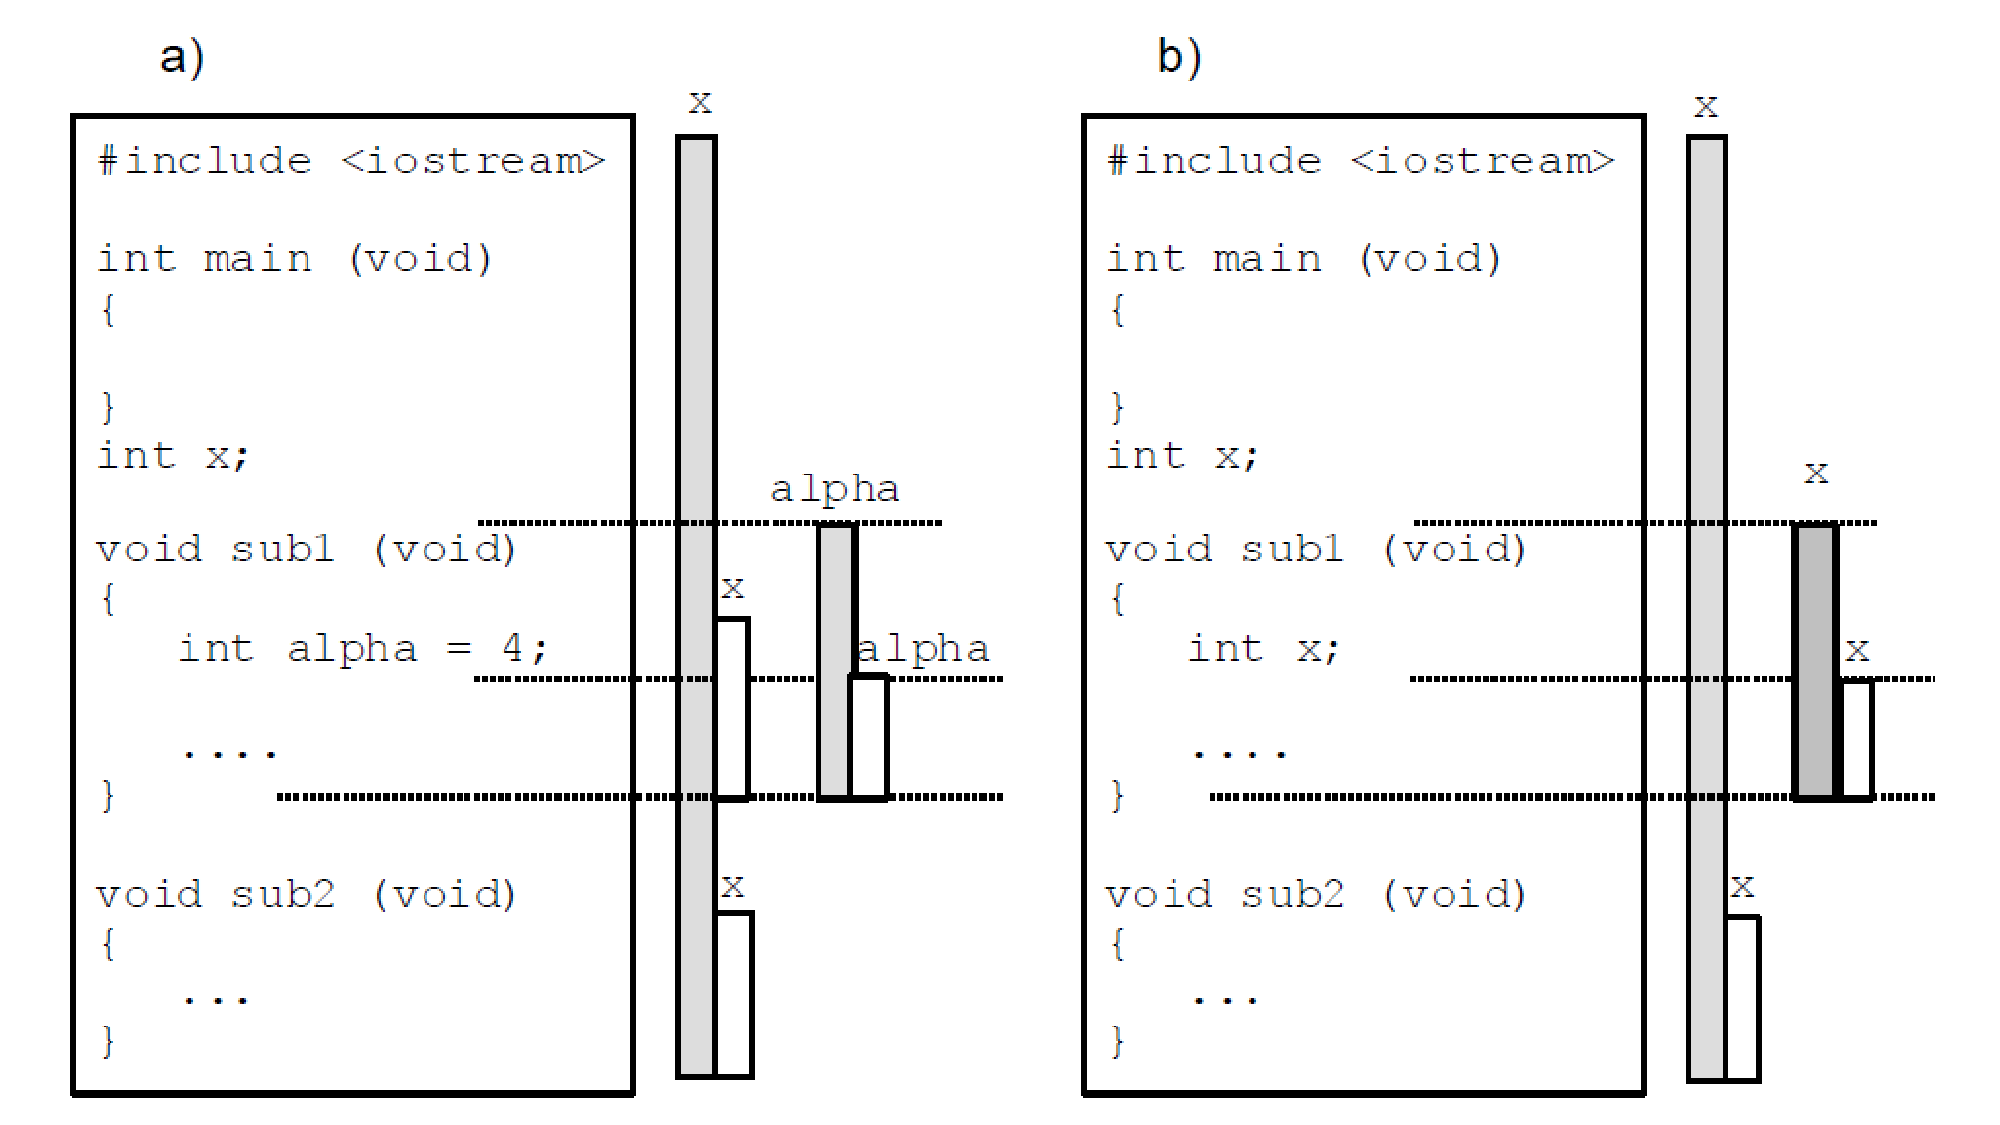
\includegraphics[width=0.7\linewidth]{scope1.pdf}
\end{figure}

\subsubsection{Codierstil\hfill}
\label{sec:unterunterabschnitt}
\begin{itemize}
	\item Variablen so lokal wie möglich definieren, d.h. im innersten möglichen Block (Tipp: nur am Anfang eines Blocks)
	\item Globale Variablen wenn immer möglich vermeiden. Sie müssen speziell gekennzeichnet werden. Sie sollen (in C) mit einem Prefix (Modulkürzel) gefolgt von einem underscore character (\_) beginnen. Dadurch werden die Namen eindeutig.
	\item[\-] Beispiel:\\Die globale Variable counter im Modul Foo muss wie folgt definiert werden:
	\noindent
\begin{minipage}{\linewidth}
\begin{lstlisting}
int Foo_counter;
\end{lstlisting}
\end{minipage}
	\item Globale Variablen am Anfang der Datei definieren, d.h. auf jeden Fall vor der ersten Funktion
\end{itemize}
\begin{hinweis}
Besser (in C++): Namespace definieren
\end{hinweis}

% Unterkapitel: Namensräume (Namespaces)

\subsection{Namensräume (Namespaces)\hfill}
\label{sec:unterabschnitt}

\subsubsection{Namensräume\hfill}
\label{sec:unterunterabschnitt}
\textbf{Namen, die zu verschiedenen Namensräumen gehören, dürfen auch innerhalb desselben Gültigkeitsbereichs gleich sein.}
In C gibt es die folgenden Namensräume (gilt auch für C++):
\begin{itemize}
	\item Marken
	\item Namen von Strukturen, Unions und enums
	\item Jede Struktur und Union für ihre Feldnamen
	\item Bezeichner von Variablen, Funktionen, typedef-Namen, enum-Konstanten
\end{itemize}
In C++ können zusätzlich explizit definierte Namensräume verwendet werden.\\
\begin{hinweis}
Dadurch können (und sollen unbedingt!) die in C üblichen Modulkürzel vermieden werden.
\end{hinweis}

\subsubsection{Explizite Namensräume in C++\hfill}
\label{sec:unterunterabschnitt}
\begin{itemize}
	\item Nebst den vordefinierten (impliziten) Namensräumen des vorherigen Abschnitts können in C++ explizit eigene Namensräume (namespaces) definiert werden.
	\item Bezeichner müssen nur innerhalb ihres Namensraums eindeutig sein
	\item Für jedes Modul in C (mit Modulkürzel) soll in C++ ein Namensraum definiert werden
	\item Sie haben bisher in allen C++-Übungen bereits den Namensraum std verwendet
\end{itemize}

\subsubsection{C++-Mechanismen für Namespaces\hfill}
\label{sec:unterunterabschnitt}
\begin{itemize}
	\item Deklaration von Namespaces
	\item Namespace-Alias
	\item[\-] Einem bestehenden Namespace einen anderen Namen zuweisen (eher selten)
\noindent
\begin{minipage}{\linewidth}
\begin{lstlisting}
namespace fbssLib = financial_branch_and_system_service_library;
\end{lstlisting}
\end{minipage}
	\item using-Deklaration
	\item using-Direktive
\end{itemize}

\subsubsection{Deklaration von Namespaces\hfill}
\label{sec:unterunterabschnitt}
\begin{itemize}
	\item Alle in einem Namespace deklarierten Bezeichner werden diesem Namespace zugeordnet
	\item Auf die Bezeichner des Namespaces kann mit dem Scope-Operator :: zugegriffen werden
	\item Syntax:
	\item[\-] Hinter dem Schlüsselwort namespace folgt der Name des Namespaces gefolgt von einem Block
	\item Innerhalb einer Datei kann mehr als ein Namespace deklariert werden (eher unüblich) und ein Namespace kann in mehreren Dateien deklariert sein (häufig, d.h. die Elemente eines Namespaces werden in mehreren Dateien implementiert)
\end{itemize}

\subsubsection{Deklaration von Namespaces: Beispiel\hfill}
\label{sec:unterunterabschnitt}
\noindent
\begin{minipage}{\linewidth}
\begin{lstlisting}
namespace myLib1
{
	int i;
	void foo();
}

namespace myLib2
{
	int i;
	void foo();
	int go();
}

...
{
	myLib1::foo();	// vollstaendiger Name von foo()
	myLib2::i = 17;	// vollstaendiger Name von i
}
\end{lstlisting}
\end{minipage}

\subsubsection{using-Deklaration\hfill}
\label{sec:unterunterabschnitt}
\begin{itemize}
	\item Eine using-Deklaration ''importiert'' Namen aus einem Namensraum und macht ihn ohne explizite Namensraumangabe verwendbar
	\item Sie kann lokal in einem Block oder global ausserhalb eines Blocks verwendet werden
	\item Deklariert nur einzelne Namen
\end{itemize}
\noindent
\begin{minipage}{\linewidth}
\begin{lstlisting}
int main()
{
	using myLib1::foo;	// lokales Synonym
	foo();			// ruft myLiby::foo() auf
}
\end{lstlisting}
\end{minipage}

\subsubsection{using-Direktive\hfill}
\label{sec:unterunterabschnitt}
\begin{itemize}
	\item Eine using-Direktive macht alle Namen aus einem Namensraum ohne explizite Namensraumangabe verwendbar
\end{itemize}
\noindent
\begin{minipage}{\linewidth}
\begin{lstlisting}
usting namespace myLib1;	// ''importiert'' alle Namen aus myLib1

int main()
{
	foo();			// ruft myLib1::foo() auf
}
\end{lstlisting}
\end{minipage}

\subsubsection{using namespace kann zu Konflikten führen\hfill}
\label{sec:unterunterabschnitt}
\begin{itemize}
	\item Wenn bei mehreren using namespace-Deklarationen und/oder -Direktiven die Namen (ohne Namespace-Angabe) nicht eindeutig sind, müssen die Namen voll qualifiziert verwendet werden (mit Namespace-Angabe)
\end{itemize}
\noindent
\begin{minipage}{\linewidth}
\begin{lstlisting}
namespace myLib1
{
	int i;
	void foo();
}

namespace myLib2
{
	int i;
	void foo();
	int go();
}

...
{
	myLib1::foo();	*@\color{red}//ist nicht eindeutig, Compiler reklamiert@*
	myLib2::i = 17;	// vollstaendiger Name von i
}
\end{lstlisting}
\end{minipage}

\subsubsection{Namenlose Namespaces\hfill}
\label{sec:unterunterabschnitt}
\begin{itemize}
	\item Ein namenloser Namespace wird wie ein spezieller Namensraum mit einem systemweit eindeutigen Namen behandelt
\end{itemize}
\begin{hinweis}
Es ist guter Programmierstil, den Gültigkeitsbereich aller nur intern verwendeten Funktionen und Daten mit Hilfe von namenlosen Namespaces auf den Bereich eingrenzen, in dem die Objekte verwendet werden. (In C hat man dafür die Funktionen mit static gekennzeichnet
\end{hinweis}
\noindent
\begin{minipage}{\linewidth}
\begin{lstlisting}
namespace
{


}
\end{lstlisting}
\end{minipage}

\subsubsection{Zugriff auf globale Variable mit Scope-Operator\hfill}
\label{sec:unterunterabschnitt}
\noindent
\begin{minipage}{\linewidth}
\begin{lstlisting}
int zahl = 11;	// globale Variable

int main()
{
	int zahl = 22;		// lokale Variable
	zahl = zahl + 4;	// lokale Variable
	::zahl = 23;		// Zugriff auf globale Variable
}
\end{lstlisting}
\end{minipage}

% Unterabschnitt: Speicherklassen

\subsection{Speicherklassen\hfill}
\label{sec:unterabschnitt}

\subsubsection{Speicherklassen in C++\hfill}
\label{sec:unterunterabschnitt}
\begin{itemize}
	\item auto
	\item[\-] Ist default, wenn nichts geschrieben wird. Eine mit auto deklarierte Variable wird nach Beendigung des Scopes automatisch entfernt.\\
	Achtung: hat ab C++11 eine andere Bedeutung!!
	\item register
	\item[\-] Ist dasselbe wie auto mit zusätzlichem Hinweis an Compiler: wenn es geht in ein Register legen (sehr zurückhaltend einsetzen, besser gar nicht)
	\item static
	\item extern
	\item mutable
	\item[\-] (später im Zusammenhang von Klassen)
\end{itemize}

\subsubsection{Speicherklasse static: Variablen\hfill}
\label{sec:unterunterabschnitt}
\begin{itemize}
	\item static-Variablen sind im Datenbereich, nicht auf dem Stack
	\item Sie werden automatisch auf 0 initialisiert, wenn nichts anderes steht
	\item Gültigkeitsbereich ist der Block, in dem die Variable definiert ist
	\item static-Variablen, welche ausserhalb einer Funktion definiert sind (globale Variablen). sind nur in der Datei gültig, in der sie definiert werden
	\item static-Variablen sind nur einmal vorhanden (auch in multi-threading-Umgebungen), d.h. ihr Wert wird erhalten, auch wenn die Funktion beendet ist. Beim nächsten Aufruf der Funktion geht es mit dem alten Wert weiter.\color{\ownRed}
	\item Nur einsetzen, wenn man das will!\color{black}
\end{itemize}

\subsubsection{Speicherklasse static: Funktionen\hfill}
\label{sec:unterunterabschnitt}
\begin{itemize}
	\item static-Funktionen sind nur in der Datei, in welcher sie definiert sind, sichtbar
	\item Alle Funktionen, welche nicht aussen (für andere Units) sichtbar sein sollen, sollten deshalb \textbf{in C} als static definiert werden\color{\ownRed}
	\item In C++ können dafür namenlose Namespaces verwendet werden (bevorzugt)\color{black}
\end{itemize}

\subsubsection{Speicherklasse extern: Externe Variablen\hfill}
\label{sec:unterunterabschnitt}
\begin{itemize}
	\item Eine externe Variable kann nur in einer einzigen Datei definiert werden (ohne Speicherklasse extern)
	\item In den anderen Dateien wird sie mit extern deklariert (bekannt gemacht)
	\item Eine manuell Initialisierung ist nur bei der Definition möglich
	\item Globale Variablen, welche nicht manuell initialisiert werden, werden automatisch mit 0 initialisiert
	\item extern-Deklarationen werden üblicherweise in einer Headerdatei deklariert und am Beginn der Datei mit \#include eingefügt
\end{itemize}

\subsubsection{Typqualifikationen (Kap. 9.2.2)\hfill}
\label{sec:unterunterabschnitt}
\begin{itemize}
	\item const
	\item[\-] const-Objekte können nicht verändert werden (read-only)
	\item volatile
	\item[\-]Der Compiler wird angewiesen, keine Optimierungen (soweit sie die Variable betreffen) vorzunehmen
	\item volatile wird oft bei Embedded Systems angewandt, wenn z.B. ''hinter'' einer Variable ein Register liegt.
	\item const und volatile können auch kombiniert werden, z.B. bei read-only-Hardwareregistern
\end{itemize}

\subsubsection{Funktionsattribute\hfill}
\label{sec:unterunterabschnitt}
\begin{itemize}
	\item inline
	\item[\-] bereits bekannt
	\item virtual
	\item[\-] später im Zusammenhang mit Klassen
	\item explicit
	\item[\-] später im Zusammenhang mit Klassen
\end{itemize}

% Unterkapitel: Typdefinitionen

\subsection{Typdefinitionen\hfill}
\label{sec:unterabschnitt}

\subsubsection{typedef zur Vereinbarung eigener Datentypen\hfill}
\label{sec:uterunterabschnitt}
\begin{itemize}
	\item analog C
	\item In C++ kann aber z.B. bei structs das typedef weggelassen werden
	\item In C:
	\item[\-]
\noindent
\begin{minipage}{\linewidth}
\begin{lstlisting}
typedef struct {int x;
		iny;} Point;
\end{lstlisting}
\end{minipage}
	\item In C++:
	\item[\-]
\noindent
\begin{minipage}{\linewidth}
\begin{lstlisting}
struct Point {
	int x;
	int y;
};
\end{lstlisting}
\end{minipage}
	\item Stil: eigene Typen werden mit einem Grossbuchstaben begonnen
\end{itemize}

\subsubsection{Beispiel\hfill}
\label{sec:unterunterabschnitt}
\noindent
\begin{minipage}{\linewidth}
\begin{lstlisting}
struct Point {
	int x;
	int y;
};

struct Line {
	Point p1;
	Point p2;
};

int main(void)
{
	line myLine = {12, -34,		// p1
			783, 12};	// p2
		
	std::cout << ''Startpunkt: ('' << myLine.p1.x << '', ''
					<< myLine.p1.y << '')\n'';
	std::cout << ''Endpunkt: ('' << myLine.p2.x << '', ''
					<< myLine.p2.y << ''\n'';
	return 0;
}
\end{lstlisting}
\end{minipage}

\subsubsection{Gewährleistung von Portabilität\hfill}
\label{sec:unterunterabschnitt}
\begin{itemize}
	\item Oft muss z.B. ein Register ein 16 Bit breiter Wert geschrieben werden. Welcher Typ ist nun 16 Bit breit?
	\item Das ist implementationsabhängig (vielleicht unsigned short, unsigned int, ...)
	\item Um die Portabilität (Umschrieben auf ein anderes System) zu vereinfachen, wird ein 16 Bit breiter Datentyp (Word) definiert und dann ausschliesslich verwendet (in stddef.h sind diese Typen üblicherweise bereits definiert). Auf einem anderen System ist dann nur noch dieser typedef zu ändern.
	\item[\-] 
\noindent
\begin{minipage}{\linewidth}
\begin{lstlisting}
typedef unsigned short uint16_t;
\end{lstlisting}
\end{minipage}
\end{itemize}

\subsubsection{Wie setzt der Compiler ein typedef um?\hfill}
\label{sec:unterunterabschnitt}
\begin{itemize}
	\item Ein typedef ist mehr oder weniger eine reine Textersetzung. Erklärung anhand des folgenden Beispiels:
	\item[\-]
\noindent
\begin{minipage}{\linewidth}
\begin{lstlisting}
typedef struct {int x;
		int y;} Point;
\end{lstlisting}
\end{minipage}
	\item Überall im Code, wo nun das Wort Point gefunden wird, ersetzt der Compiler dieses in einem ersten Durchgang mit dem Text 
	\item[\-]
\noindent
\begin{minipage}{\linewidth}
\begin{lstlisting}
typedef struct {int x;
		int y;}
\end{lstlisting}
\end{minipage}	
\end{itemize}

\subsection{Initialisierung\hfill}
\label{sec:unterabschnitt}
\begin{itemize}
	\item analog C
\end{itemize}

\subsection{Type-Case (Typumwandlungen)\hfill}
\label{sec:unterabschnitt}

\subsubsection{Typumwandlungen im Allgemeinen\hfill}
\label{sec:unterunterabschnitt}
\begin{itemize}
	\item Unsafe conversion
	\item[\-] Wenn bei der Typumwandlung signifikante Stellen verloren gehen können (typischerweise bei einer Umwandlung von einem ''grösseren'' in einen ''kleineren'' Typ, z.B. von double nach int)
	\item[\-] Bei int ist siwihl die Genauigkeit als auch die maximal darstellbare Zahl
	\item Safe conversion
	\item[\-] Wenn bei der Typumwandlung keine signifikanten Stellen verloren gehen können (typischerweise bei einer Umwandlung von einem ''kleineren'' in einen ''grösseren'' Typ, z.B. von in nach double
\end{itemize}

\subsubsection{Implizite Typumwandlung\hfill}
\label{sec:unterunterabschnitt}
\begin{itemize}
	\item Die implizite (automatische) Typumwandlung wird auch als Standard-Typumwandlung bezeichnet
	\item Sie erfolgt analog zur Programmiersprache C (siehe dort)
\end{itemize}

\subsubsection{Explizite Typumwandlung\hfill}
\label{sec:unterunterabschnitt}
\begin{itemize}
	\item Nebst den impliziten (automatischen) Typumwandlungen kann in C++ mit Hilfe von 6 verschiedenen cast-Operatoren eine explizite Typumwandlung bewirkt werden.
	\item Bei der expliziten Typumwandlung gibt der Programmierer explizit an, was er will.
	\item[\-]
	\begin{achtung}
	Bei der expliziten Typumwandlung übernimmt der Programmierer die Verantwortung, dass die Umwandlung keine Probleme ergibt.\\
	(z.B. Umwandlung von grosser Zahl in kleineren Typ)
	\end{achtung}
\end{itemize}

\subsubsection{Explizite Typumwandlung \#1, 2: C-Stil und Funktionsstil\hfill}
\label{sec:unterunterabschnitt}
\begin{itemize}
	\item Stroustrup: ''The C and C+ cast is a sledgehammer...''
	\item Syntax für C-Stil (einzige Variante in C):
	\item[\-](Zieltyp)expression
	\item[\-]
\noindent
\begin{minipage}{\linewidth}
\begin{lstlisting}
int a = (int)4.6;	// a == 4
\end{lstlisting}
\end{minipage}
	\item Syntax für Funktionsstil:
	\item[\-] Zieltyp(expression)
	\item[\-]
\noindent
\begin{minipage}{\linewidth}
\begin{lstlisting}
int a = int(4.6);	// a == 4
\end{lstlisting}
\end{minipage}
\end{itemize}

\subsubsection{Typumwandlung mit C-Stil und Funktionsstil\hfill}
\label{sec:unterunterabschnitt}
\textbf{Typumwandlung ist...}
\begin{itemize}
	\item einfache Reinterpretation der bitweisen Darstellung des Ausdrucks
	\item einfache arithmetische Grössenanpassung
	\item ein const- oder volatile-Attribut zu einem Ausdruck hinzufügen oder entfernen
	\item andere (eventuell implementierungsabhängige) Umwandlung
\end{itemize}
\begin{achtung}
Aus dem Sourcecode geht nicht hervor, welche der aufgeführten Typumwandlungen der Programmierer wollte.\\ 
Diese beiden Casts sollten in C++ nicht verwendet werden!
\end{achtung}

\subsubsection{Explizite Typumwandlung \#3: const\_cast\hfill}
\label{sec:unterunterabschnitt}
\textbf{Anwendung:}\\
Ausschliesslich die (vorübergehende) Entfernung des const-Qualifikators, d.h. die Umwandlung eines Ausdrucks vom Typ T mit den optionalen Qualifikatoren const und volatile in einen Ausdruck desselben Typs ohne den Qualifikator const\\
\textbf{Syntax:}
\noindent
\begin{minipage}{\linewidth}
\begin{lstlisting}
const_cast<Zieltyp>expression

const char* findSubString(const char* str, const char* subStr)
{
	return strstr(const_cast<char*<str,
			const_cast<char*>subStr);
}
\end{lstlisting}
\end{minipage}
Die Funktion strstr() akzeptiert nur Parameter com Typ char* (ohne const)

\subsubsection{Explizite Typumwandlung \#4: static\_cast\hfill}
\label{sec:unterunterabschnitt}
\textbf{Anwendung:}\\
Umwandlung von Objekten einer Klasse auf Objekte einer Basisklasse oder die Umwandlung mittels einer Umwandlungsfunktion.\\
Wenn schon Type cast, dann ist static\_cast die häufigste.

\subsubsection{Explizite Typumwandlung \#5: dynamic\_cast\hfill}
\label{esc:unterunterabschnitt}
\textbf{Anwendung:}\\
Umwandlung von polymorphen Objekten im Zusammenhang mit dem Typsystem von C++ eingesetzt (Stichwort RTTI = Runtime Type Information System)\\
Näheres folgt später im Zusammenhang mit Klassen und Polymorphismus.

\subsubsection{Explizite Typumwandlung \#6: reinterpret\_cast\hfill}
\label{sec:unterunterabschnitt}
\textbf{Anwendung:}\\
reinterpret\_cast ist eine neue Interpretation der zugrunde liegenden Bitkette.\\
\textbf{Syntax:}
\noindent
\begin{minipage}{\linewidth}
\begin{lstlisting}
reinterpret_cast<Zieltyp>expression

char* p = new char[20];
...
int* pi = reinterpret_cast<int*>p;
\end{lstlisting}
\end{minipage}



\clearpage
%!TEX root = main.tex

\section{Kapitel 6: Module und Datenkapseln\hfill}
\label{sec:Kapitel 6: Module und Datenkapseln}

\subsection{Modul (Unit)\hfill}
\label{sec:Modul (Unit)}

\subsubsection{Motivation\hfill}
\label{sec:Motivation}
\begin{itemize}
	\item \textbf{Arbeitsteilung}
	\item[\-] Grosse Programme werden von mehreren Personen entwickelt. Praktikabel ist, wenn nur eine Person an einer bestimmten Datei arbeitet.
	\item \textbf{Effizienz}
	\item[\-] Eine Übersetzungseinheit (Datei) muss bei jeder Änderung neu übersetzt werden (je grösser die Datei desto langsamer die Übersetzung)
	\item \textbf{Strukturierung}
	\item[\-] Ein grosses  Programm in mehrere vernünftige Teile (Baugruppen, Units) aufteilen (Divide and conquer)
\end{itemize}

\subsubsection{Nomenklatur: Modul vs. Unit\hfill}
\label{sec:Nomenklatur: Modul vs. Unit}
\begin{itemize}
	\item Ein Programmbaustein wird traditionell mit Modul (der oder das Modul) bezeichnet
	\item Der Test eines Moduls heisst folglich Modultest
	\item Das Vorgehen, welches Module generiert, heisst Modularisierung
	\item Heute üblicher wird Modul mit Unit, der Test mit Unittest bezeichnet, das Vorgehen heisst weiterhin Modularisierung
	\item Prinzipiell spreche ich künftig meist von Unit und Unittest
\end{itemize}

\subsubsection{Ziele der Modularisierung\hfill}
\label{sec:Ziele der Modularisierung}
\begin{itemize}
	\item Klare, möglichst schlanke Schnittstellen definieren
	\item Units so bilden, dass Zusammengehörendes in einer Unit isoliert wird (Kohäsion) soll hoch sein
	\item Schnittstellen zwischen den Units sollen klein sein (Kopplung soll klein sein)
	\item Abhängigkeiten unter den Units sollen eine Hierarchie bilden, zirkuläre (gegenseitige) Abhängigkeiten müssen vermieden werden
\end{itemize}

\subsubsection{Eigenschaften einer Unit (eines Moduls)\hfill}
\label{sec:Eigenschaften einer Unit (eines Moduls)}
\begin{itemize}
	\item realisiert eine in sich abgeschlossene Aufgabe
	\item kommuniziert über ihre Schnittstelle mit der Umgebung
	\item kann ohne Kenntnisse ihres inneren Verhaltens in ein Gesamtsystem integriert werden
	\item ihre Korrektheit kann ohne Kenntnis ihrer Einbettung in einem Gesamtsystem nachgewiesen werden (mittels Unittest)
\end{itemize}

\subsubsection{Bestandteile eine C++-Programms\hfill}
\label{sec:Bestandteile eine C++-Programms}
\begin{itemize}
	\item \textbf{Eine} Hauptfunktion main()
	\item Eine Reihe von unabhängigen Programmbausteinen (Units)
\end{itemize}

\subsubsection{Unitkonzept\hfill}
\label{sec:Unitkonzept}
\begin{itemize}
	\item Interface definiert die Schnittstelle, d.h. die Deklarationen wie Funktionsprototypen, etc. (Schaufenster)
	\item Implementation: In diesem Teil sind die Unterprogramme definiert, d.h. auscodiert (Werkstatt)
	\item Das Interface wird in einer Headerdatei (*.h) beschrieben, die Implementation liegt in einer *.cpp-Datei
\end{itemize}
\noindent
\begin{figure}[hh]
	\centering
	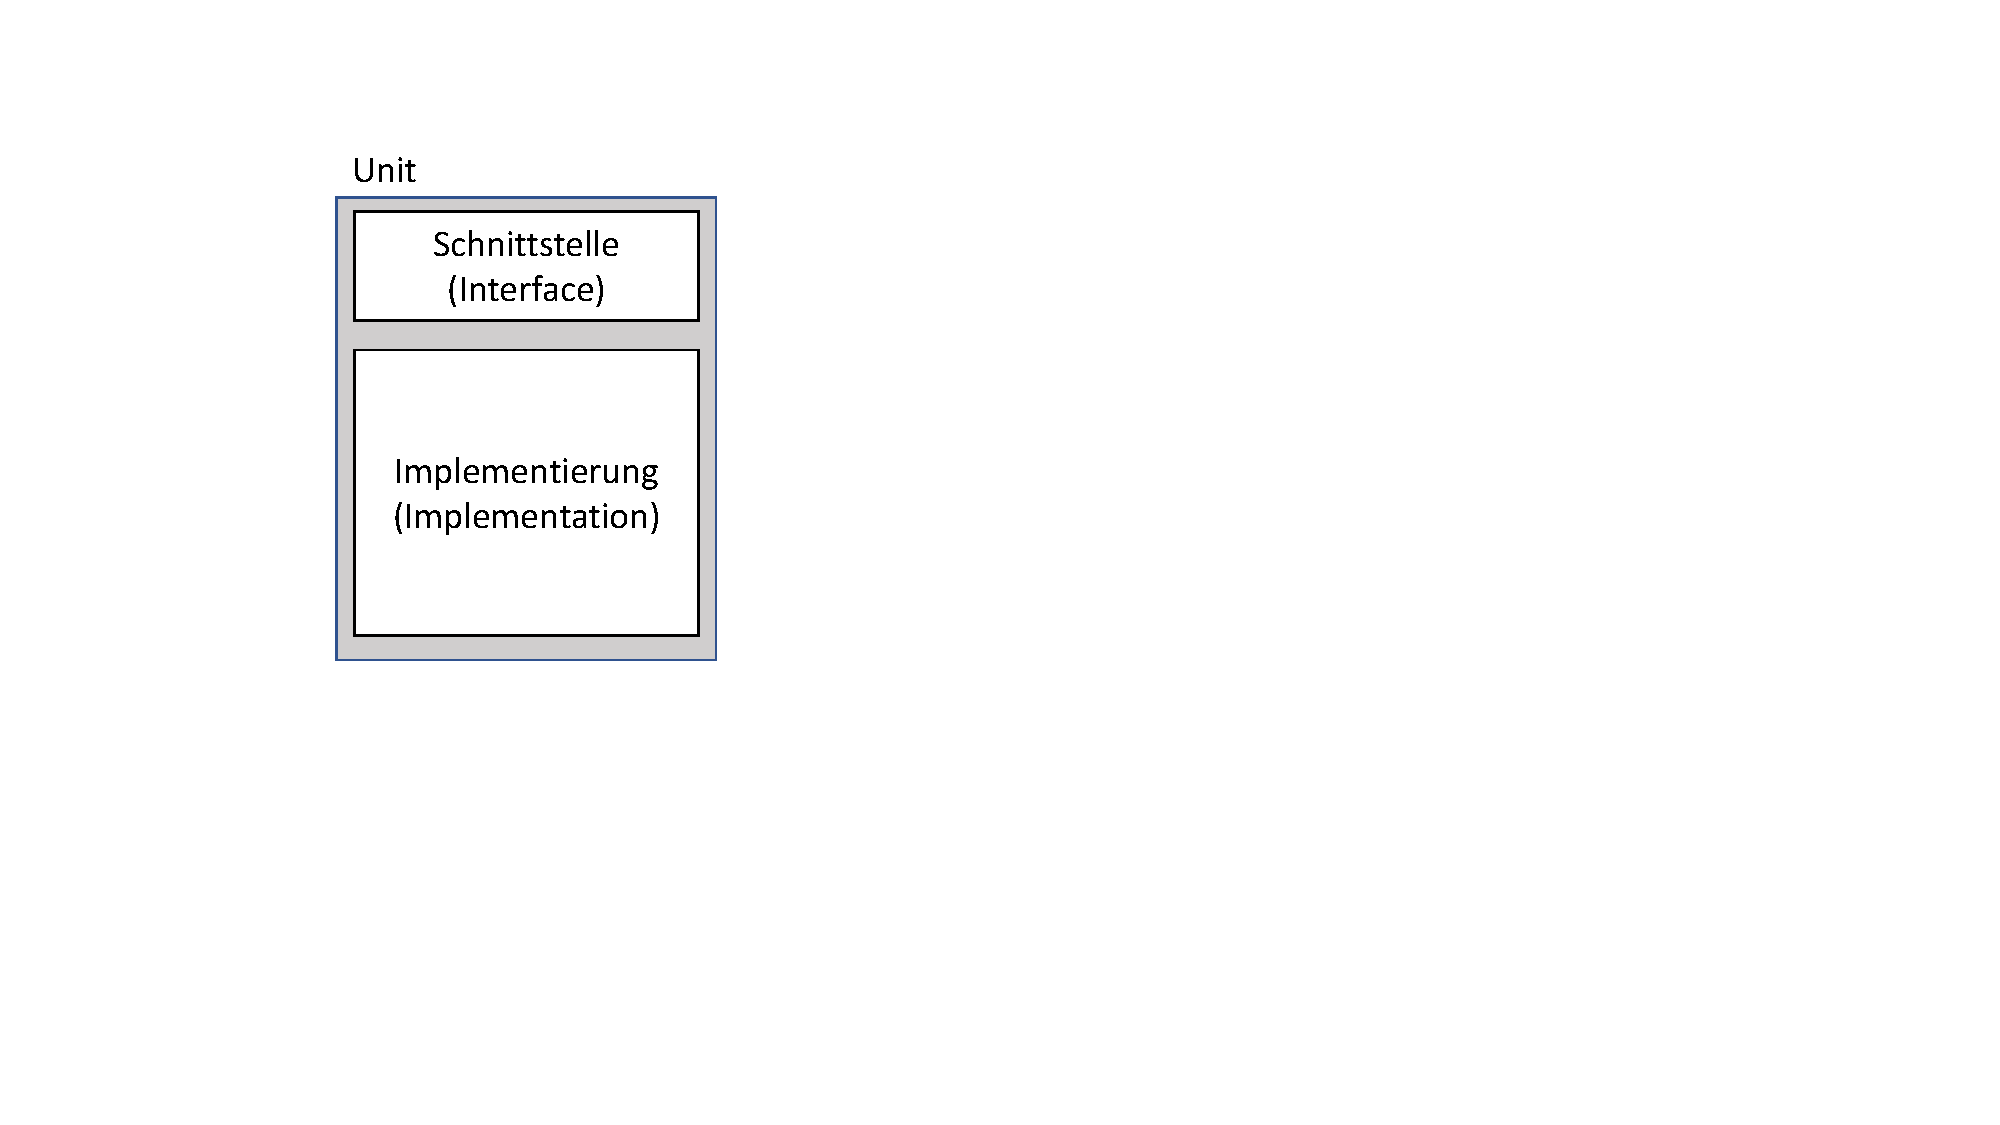
\includegraphics[width=0.3\linewidth]{unit1.pdf}
\end{figure}

\subsection{Geheimnisprinpzip (Information Hiding)\hfill}
\label{sec:Geheimnisprinzip (Information Hiding)}

\subsubsection{Information Hiding\hfill}
\label{sec:Information Hiding}
\begin{itemize}
	\item In der Schnittstelle (Headerdatei) wird alles beschrieben, was ein Nutzer dieser Unit wissen muss
	\item Der innere Aufbau der Unit (*.cpp) muss (darf) dem Nutzer der Unit nicht bekannt sein, er benötigt diese Informationen auch gar nicht
	\item Der Nutzer der Unit darf keine Annahmen bezüglich des inneren Aufbaus der Unit treffen
	\item Der Entwickler der Unit darf den inneren Aufbau der Unit ändern, solange dadurch die Schnittstelle nicht geändert werden muss
\end{itemize}

\subsubsection{Konzept der Datenkapsel\hfill}
\label{sec:Konzept der Datenkapsel}
\begin{itemize}
	\item Eine Unit besteht aus Funktionen und Daten
	\item In der Schnittstelle wird definiert, was für den Nutzer zur Verfügung steht. Dies können Funktionen und Daten sein
	\item Die Datenkapsel fordert nun zusätzlich, dass auf die Daten nicht direkt zugegriffen werden darf, sondern nur über Zugriffsfunktionen
\end{itemize}

\subsubsection{Beispiel für Datenzugriff bei Datenkapsel\hfill}
\label{sec:Beispiel fuer Datenzugriff bei Datenkapsel}
\noindent
\begin{minipage}{\linewidth}
	\begin{lstlisting}
	// interne Daten
	int counter;	// gehoert zur Unit, nicht in Interface
			// wie kann das in C bewerkstelligt werden?
		
	// Schnittstelle (Interface)
	voi setCounter(int c)
	{
		counter = c;
	}
	
	int getCounter(void)
	{
		return counter;
	}
	\end{lstlisting}
\end{minipage}

\subsubsection{Beispiel für Unit Rechteck (ohne Datenkapsel)\hfill}
\label{sec:Beispiel fuer Unit Rechteck (ohne Datenkapsel)}
\noindent
\begin{minipage}{\linewidth}
	\begin{lstlisting}
	// interne Daten
	double a;	// 1. Seite
	double b;	// 2. Seite
	double area;	// Rechtecksflaeche
	
	// Schnittstelle (Interface)
	
	// direkter Zugriff auf a, b, area
	// Annahme: area hat immer den aktuellen Wert, d.h. es muss
	// bei jeder Aenderung von a und b (durch den Client!) berechnet werden
	\end{lstlisting}
\end{minipage}
\begin{achtung}
	Sehr gefährlich! (kann kaum sichergestellt werden)
\end{achtung}

\subsubsection{Beispiel für Unit Rechteck: Verbesserung \#1}
\label{sec:Beispiel fuer Unit Rechteck: Verbesserung 1}
\noindent
\begin{minipage}{\linewidth}
	\begin{lstlisting}
	// interne Daten
	double a;	// 1. Seite
	double b;	// 2. Seite
	double area;	// Rechtecksflaeche
	
	// Schnittstelle (Interface)
	// kein direkter Zugriff mehr auf a, b, area
	// Funktionen setA(), setB(), getA(), getB(), getArea()
	void setA(double newA)
	{
		a = newA;
		area = a * b;
	}
	
	double getArea(void)
	{
		return area;
	}
	\end{lstlisting}
\end{minipage}
\begin{hinweis}
	Evtl. gefährlich (Berechnung von area könnte vergessen werden). Und: soll die Multiplikation wirklich bei jeder Aenderung durchgefuehrt werden?
\end{hinweis}

\subsubsection{Beispiel für Unit Rechteck: Verbesserung \#2}
\label{sec:Beispiel fuer Unit Rechteck: Verbesserung 2}
\noindent
\begin{minipage}{\linewidth}
	\begin{lstlisting}
	// interne Daten
	double a;	// 1. Seite
	double b;	// 2. Seite
	// double area;	// Rechtecksflaeche, Attribut wird entfernt
	
	// Schnittstelle (Interface)
	// Attribut area wird entfernt
	// Funktionen setA(), setB(), getA(), getB(), getArea()
	void setA(double newA)
	{
	a = newA;
	}
	
	double getArea(void)
	{
		return a * b;
	}
	\end{lstlisting}
\end{minipage}
\begin{hinweis}
	Dank Datenkapsel darf das Attribut area entfernt werden. Die Schnittstelle ändert sich dadurch nicht.
\end{hinweis}

\subsubsection{Unit nutzen\hfill}
\label{sec:Unit nutzen}
\noindent
\begin{minipage}{\linewidth}
	\begin{lstlisting}
	#include "foo.h"
	// dadurch wird die Schnittstelle der Unit foo bekanntgemacht
	\end{lstlisting}
\end{minipage}

\subsubsection{Unit-Schnittstelle definieren (in Headerdatei)\hfill}
\label{sec:Unit-Schnittstelle definieren}
\noindent
\begin{minipage}{\linewidth}
	\begin{lstlisting}
	// Datei: foo.h
	#ifndef FOO_H_
	#define FOO_H_
	
	// Deklarationen
	
	
	#endif /* FOO_H_ */
	\end{lstlisting}
\end{minipage}
\begin{hinweis}
include-Guard: verhindert das mehrfache include derselben Datei
\end{hinweis}

\subsubsection{Deklarationsreihenfolge in der Headerdatei (*.h)\hfill}
\label{sec:Deklarationsreihenfolge in der Headerdatei}
\begin{achtung}
	kein using namespace ... in Headerdateien!
\end{achtung}
\begin{enumerate}
	\item Dateikommentar
	\item \#include der verwendeten System-Header (iostream, etc.)
	\item[\-] \#include <...>
	\item \#include der projektbezogenen Header (\#include "...")
	\item Konstantendefinitionen
	\item typedefs und Definitionen von Strukturen
	\item Allenfalls extern-Deklarationen von globalen Variablen
	\item Funktionsprototypen, inkl. Kommentare der Schnittstelle, bzw. Klassendeklarationen
\end{enumerate}
\begin{hinweis}
	Punkte 2-7 sind innerhalb des inlcude-Guards.
\end{hinweis}

\subsubsection{Reihenfolge in der Implementierungsdatei (*.cpp)\hfill}
\label{sec:Reihenfolge in der Implementierungsdatei}
\begin{enumerate}
	\item Dateikommentar
	\item \#include der verwendeten System-Header (iostream, etc.)
	\item \#include der projektbezogenen Header
	\item allenfalls globale Variablen und statische Variablen
	\item Präprozessor-Direktiven
	\item Funktionsprototypen von lokalen, internen Funktionen
	\item Definition von Funktionen und Klassen
	\item[\-] \color{\ownRed} (Kommentare aus Headerdatei nicht wiederholen!)
\end{enumerate}

\subsubsection{\#include-Konzept}
\label{sec:include-Konzept}
\begin{itemize}
	\item Mit den \#includes wird oft ein Riesenchaos veranstaltet
	\item Der "Einfachheit halber" werden ab und zu einfach alle oder fast alle Headerdateien inkludiert
	\item Das muss unbedingt verhindert werden
\end{itemize}
\textbf{Regel: In jeder Datei (*.h, *.cpp, *.c) werden genau die Headerdateien inkludiert, welche diese Datei selbst benötigt!}

\subsubsection{Unit compilieren\hfill}
\label{sec:Unit compilieren}
\begin{center}
	\textbf{g++ \color{\ownRed}-c\color{black} foo.cpp}
\end{center}
\begin{itemize}
	\item Dadurch entsteht noch kein ausführbares Programm, sondern nur die Datei foo.o, der Objectcode
	\item Dies muss mit allen *.cpp-Dateien gemacht werden
\end{itemize}

\subsubsection{Units linken\hfill}
\label{sec:Units linken}
\begin{center}
	g++ -o foo foo.o goo.o hoo.o
\end{center}
\begin{itemize}
	\item Alle Objectdateien müssen gelinkt werden
	\item Dadurch werden allenfalls noch offene Verbindungen (Links) zu aufgerufenen Funktionen aufgelöst
\end{itemize}

\subsubsection{Buildprozess\hfill}
\label{sec:Buildprozess}
\begin{itemize}
	\item Der Buildprozess beinhaltet alle Schritte, um ein ausführbares Programm zu erhalten, bzw. aufzubauen (englisch to build)
	\item[\-] g++ -c foo.cpp
	\item[\-] g++ -c goo.cpp
	\item[\-] g++ -c hoo.cpp	
	\item[\-] g++ -o foo foo.o goo.o hoo.o
\end{itemize}
\begin{hinweis}
	Es wäre mühsam, wenn diese Befehle jedesmal neu eingetippt werden müssten. Deshalb wird in der Praxis oft ein Buildtool eingesetzt, z.B. make.
\end{hinweis}

\subsection{Make-Tool}
\label{sec:Makt-Tool}

\subsubsection{Abhängigkeiten zwischen Dateien}
\label{sec:Abhaengigkeiten zwischen Dateien}
\noindent
\begin{figure}[hh]
	\centering
	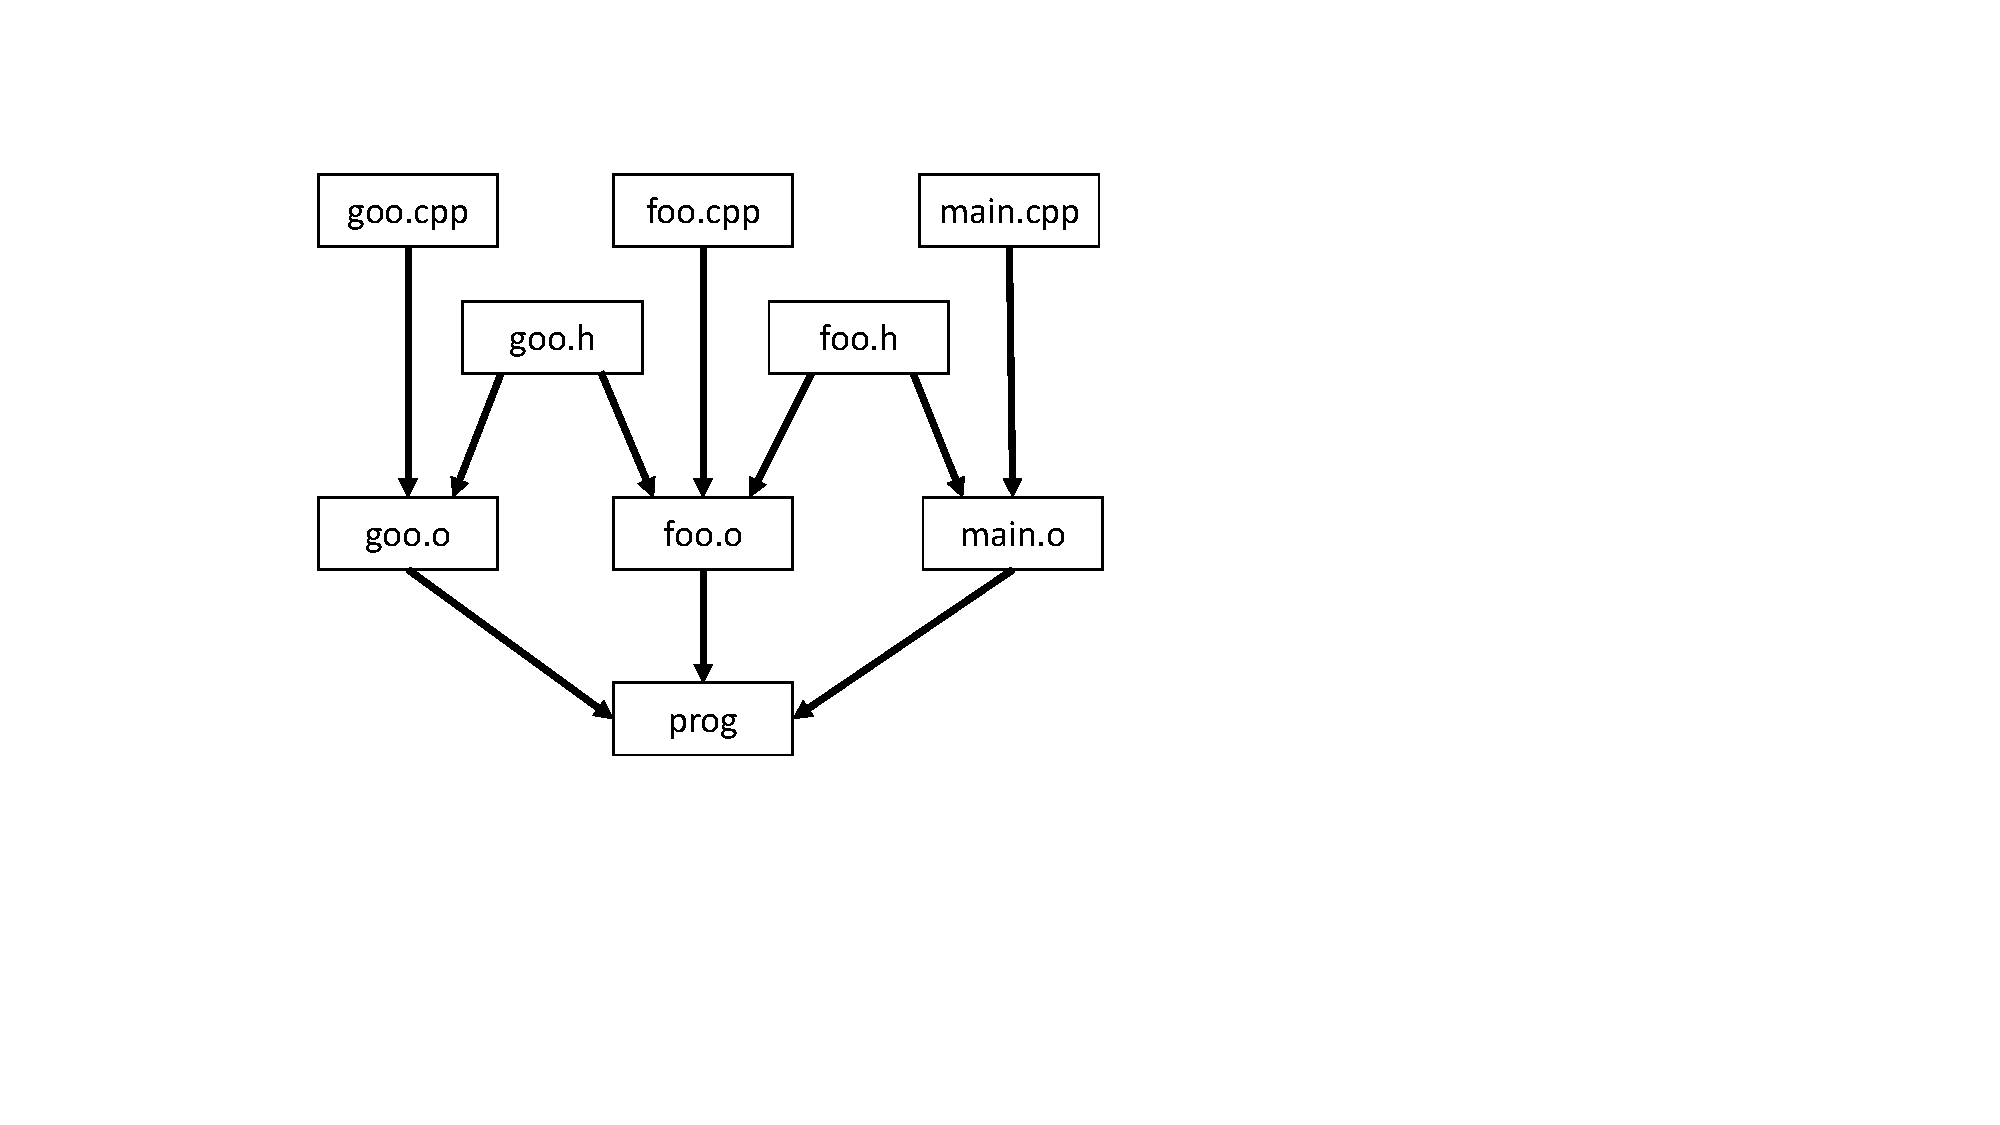
\includegraphics[width=0.5\linewidth]{make1.pdf}
\end{figure}

\subsubsection{make-File}
\label{sec:make-File}
\begin{itemize}
	\item In einem make-File können Abhängigkeiten definiert werden
	\item Wenn eine Datei geändert wurde, dann werden alle Operationen ausgeführt mit den Dateien, welche von dieser geänderten Datei abhängen
	\item Der Befehl (g++) wird z.B. nur dann ausgeführt, wenn sich an den Dateien, zu denen eine Abhängigkeit besteht, etwas geändert hat
\end{itemize}

\subsubsection{Beispiel: makefile}
\label{sec:Beispiel: makefile}
\noindent
\begin{figure}[hh]
	\centering
	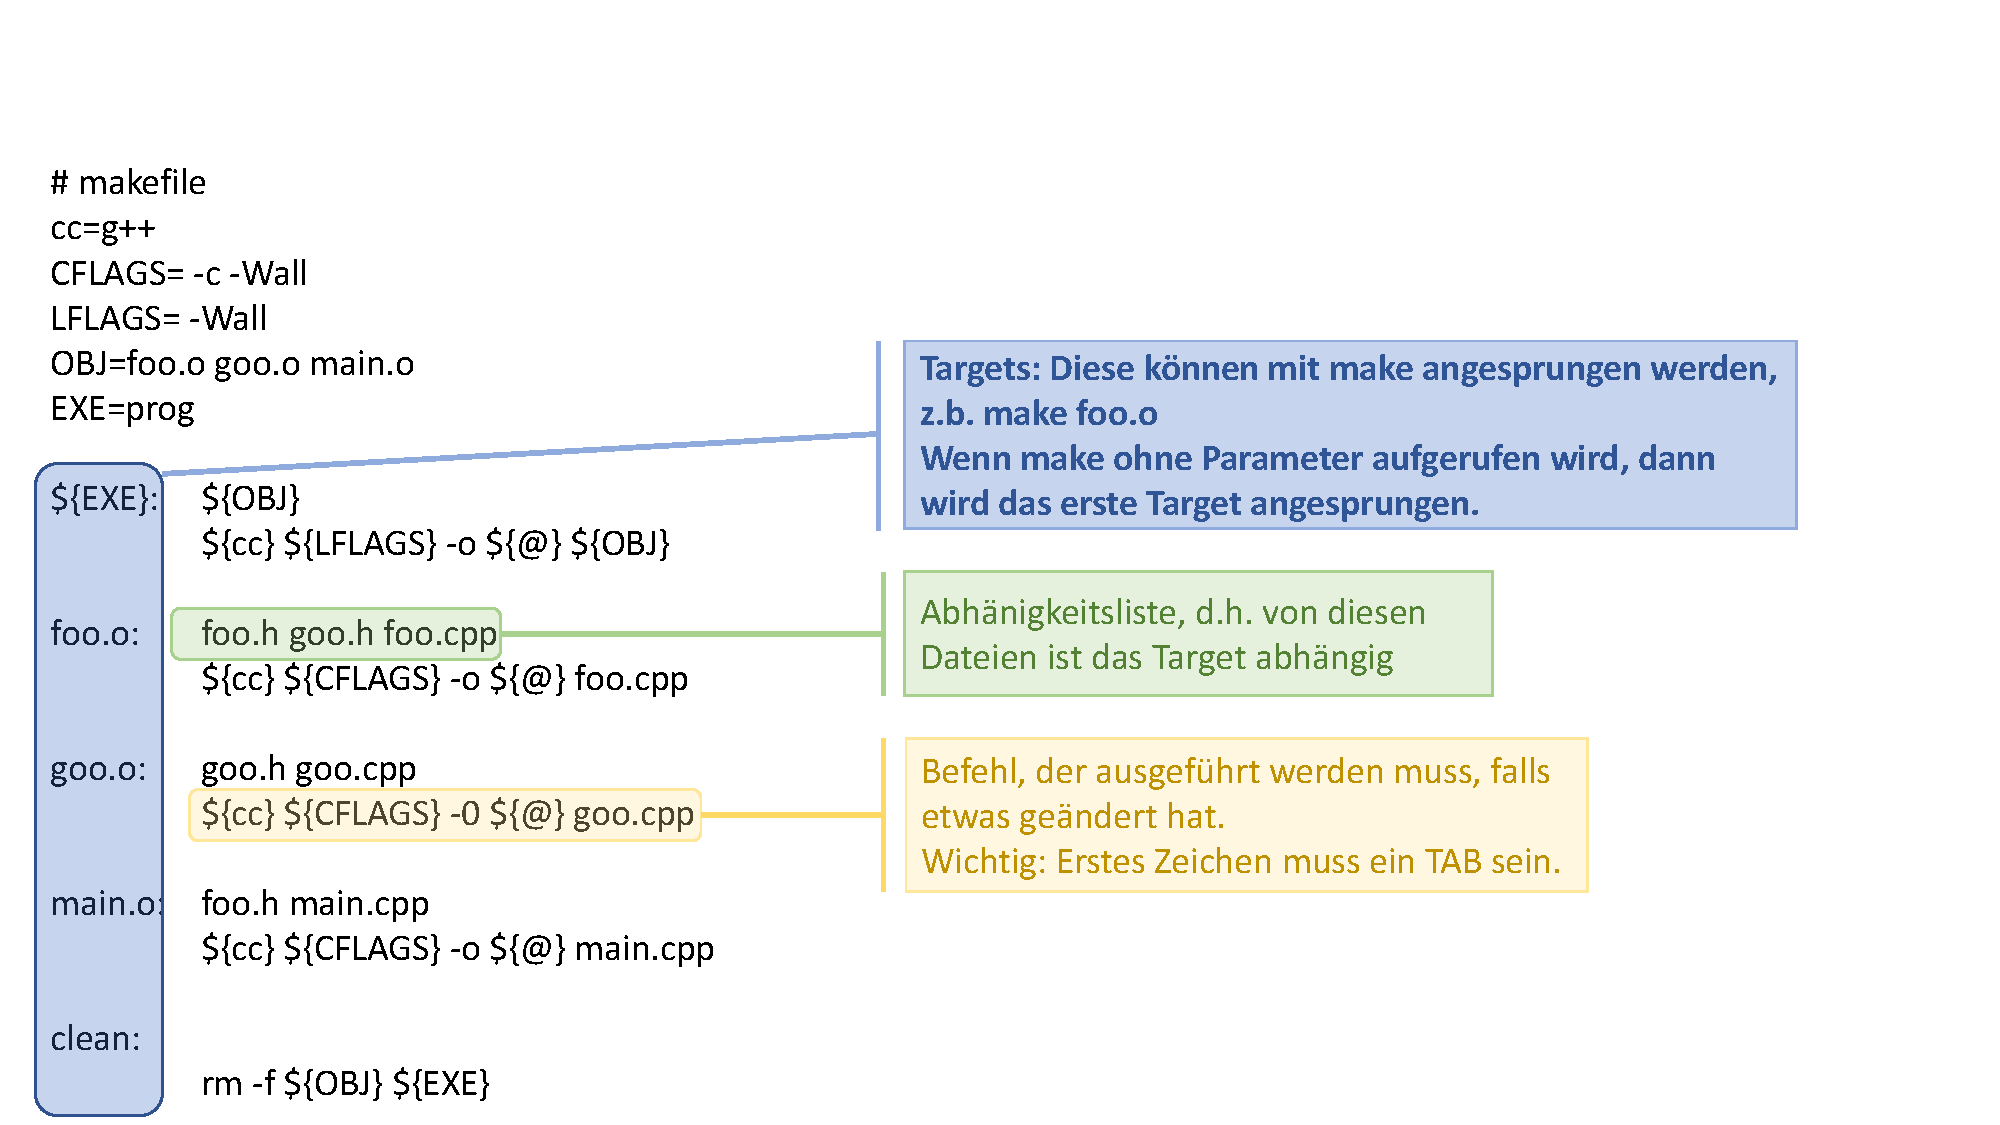
\includegraphics[width=\linewidth]{makefile.pdf}
\end{figure}
\clearpage
%!TEX root = ProgCPP_ZF.tex

\part{Eclipse IDE}

\begin{multicols}{2}
\section{Eclipse}
\begin{itemize}
	\item Integrated Development Environment
	\item[\-] (IDE, Integrierte Entwicklungsumgebung)
	\item Open-Source Software (OSS)
	\item Offene, erweiterbare Architektur basierend auf Plug-Ins
	\item Implementiert in Java
	\item Auf verschiedenen Plattformen lauffähig (multi-platform)
	\item Für unterschiedliche Programmiersprachen (multi-language)
\end{itemize}
\vfill\null
\columnbreak
\section{subWorkspace}
\begin{itemize}
	\item Der Workspace enthält vom Benutzer definierte Daten (Projekte und Ressourcen wie Ordner und Files).
	\item Er enthält alle User-Metadaten (Code, Scripts, Database objects, Konfigurationsdaten).
	\item Ein Benutzer arbeitet zu einer bestimmten Zeit genau in einem einzigen Workspace.
\end{itemize}
\end{multicols}

\begin{multicols}{2}
\subsection{Ressourcen (Resources)}
\begin{itemize}
	\item Oberbegriff für
	\begin{itemize}
		\item Projekte
		\item Ordner
		\item Files
	\end{itemize}
	\item Üblicherweise in einer hierarchischen Struktur betrachtet.
	\item Können editiert werden.
\end{itemize}
\vfill\null
\columnbreak
\subsection{Project}
\begin{itemize}
	\item Ein logisches Speicherkonzept für die Speicherung von Programmen.
	\item Gehört einem Workspace an.
	\item Ist implementiert als Verzeichnis in einem Workspace.
\end{itemize}
\end{multicols}

\subsection{Debugger}

\begin{multicols}{2}
\subsubsection{Testen und Debugging}
\begin{itemize}
	\item Testen und Debugging sind zwei unterschiedliche Prozesse.
	\item Das Ziel eines Tests ist, Fehler zu finden.
	\item Das Ziel des Debuggings ist, diese Fehler zu lokalisieren und zu korrigieren.
\end{itemize}
\vfill\null
\columnbreak
\subsubsection{Funktionen eines Debuggers}
\begin{itemize}
	\item Betrachten von Variablenwerten
	\item Unterbrechung des Programmablaufs mit Breakpoints
	\item Schrittweise Ausführung von Programmen (Step into, Step out)
\end{itemize}
\end{multicols}

\subsubsection{Assertions (Zusicherungen)}
\begin{minipage}{0.25\linewidth}
\begin{lstlisting}
#include <cassert>
assert(i>0);

// in C:
#include <assert.h>
assert(i>0);
\end{lstlisting}
\end{minipage}%
\begin{minipage}{0.75\linewidth}
\begin{itemize}
	\item Zweck: Überprüfung von logischen Annahmen während der Entwicklungsphase, speziell für die Überprüfung von Anfangs- und Endbedingungen in einer Funktion.
	\item Das Programm bricht mit einer Fehlermeldung ab, falls das Argument den booleschen Wert false besitzt. Im Beispiel oben: Abbruch, falls i <= 0.
	\item Zu beachten:
	\begin{itemize}
		\item assert() ist wirkungslos, wenn ohne Debugschalter compiliert wird. Dies ist in der (Release-)Version der Fall, die ausgeliefert wird.
		\item Bei den assert()-Anweisungen darf deshalb kein Nebeneffekt programmiert werden, da dieser in der ausgelieferten Version fehlen würde.
		\item Beispiel:
		\item[\-] assert(openFile(filename) == ok);
		\item[\-] Wenn ohne Debugschalter compiliert wird, würde das File nicht mehr geöffnet!
	\end{itemize}
\end{itemize}
\end{minipage}

\clearpage
%!TEX root = ProgCPP_ZF.tex

\part{Klassen}

\section{Objektorientierte Programmierung}

\subsection{Prozedurale vs. Objektorientierte Sicht}
Die Objektorientierte Sicht ist meist die intuitivere Sicht der Realität als die prozedurale, da physisch existierende Objekte direkt als Objekte in einem objektorientierten Design modelliert werden können.

\section{Unified Modeling Language (UML)}
\href{www.uml.org}{www.uml.org}
\vspace{-\baselineskip}
\begin{multicols}{2}
\begin{minipage}{\linewidth}
	\includegraphics[width=\linewidth]{images/klasse3.pdf}
\end{minipage}
\begin{itemize}
	\item UML ist...
	\begin{itemize}
		\item \textbf{kein} Softwareprozess-Modell
		\item \textbf{kein} Lebenszyklusmodell
		\item \textbf{keine} Programmiersprache
		\item nicht ohne Redundanz
		\begin{itemize}
			\item es gibt oft mehrere Möglichkeiten, etwas zu modellieren
		\end{itemize}
		\item \textbf{kein} Softwaretool
	\end{itemize}
\end{itemize}
\vfill\null
\columnbreak
\begin{itemize}
	\item UML ist eine graphische Modellierungssprache
	\item Ziel der UML
	\begin{itemize}
		\item fortlaufendes (objektorientiertes) Modellierungskonzept für alle Software-Entwicklungsphasen
	\end{itemize}
	\item UML ist heute der de facto Standard für die Softwaremodellierung
	\item UML ist (programmier-)sprachenunabhängig
	\item UML unterstützt den gesamten Entwicklungsprozess
	\item UML integriert (fast) alle früheren Modellierungstechniken
	\begin{itemize}
		\item Datenmodellierung
		\item Prozessmodellierung
		\item Zustands- und Verhaltensmodellierung
		\item Steuerfluss-Modellierung
	\end{itemize}
\end{itemize}
\end{multicols}

\subsection{UML-Notation der Klasse}
\begin{itemize}
	\item Eine Klasse ist der Bauplan für Objekte.
	\item Eine Klasse besteht aus Daten (Attribute) und den Funktionen (Methoden) auf diesen Daten.
	\item Sichtbarkeit:
	\begin{itemize}
		\item[\-] +: public
		\item[\-] -: private
		\item[\-] \#: protected
	\end{itemize}
\end{itemize}

\subsection{Klassenbegriff}
\begin{itemize}
	\item Eine Klasse ist eine Struktur (eine Struktur besteht nur aus Daten), die mit den Funktionen, welche auf diesen Daten arbeiten, erweitert wurde.
	\item Eine Klasse ist also eine Struktur, welche die Daten und die Funktionen auf diesen Daten in ein syntaktisches Konstrukt packt.
	\item \textbf{Die Klasse ist die Umsetzung der Datenkapsel.}
	\item Eine Klassendeklaration ist eine Typendefinition. Die "Variablen" einer Klasse werden als $"$Objekte$"$ bezeichnet.
\end{itemize}

\clearpage
\subsection{Klasse definieren und Objekte anlegen: Syntax}
Der Name der Klasse kann fast beliebig gewählt werden.\\
\textbf{Konvention:} mit Grossbuchstaben beginnen
\begin{minipage}{0.7\linewidth}
\vspace{-\baselineskip}
\begin{lstlisting}
class Classname	// Deklaration der Klasse
{
	...
};

Classname obj1;						// Objekt definieren
Classname obj2;						// Objekt definieren
Classname* objPtr;				// Objekt-Pointer definieren
Classname& objRef = obj1;	// Objekt-Referenz definieren
\end{lstlisting}
\end{minipage}

\section{Zugriffsschutz bei Klassen}
\begin{itemize}
	\item Innerhalb der Klasse hat jede Methode der Klasse auf die Elemente Zugriff. (innerhalb der Klasse sind die Methoden und Attribute der Klasse "lokale Globale")
	\item Von ausserhalb der Klasse gibt es grundsätzlich keinen Zugriff auf Klassenelemente (default, d.h. wenn nichts steht)
	\item Alles, was von aussen zugreifbar sein soll, muss explizit mit \emph{public:} gekennzeichnet werden.
	\item Obwohl nicht unbedingt notwendig, werden die nach aussen nicht sichtbaren Elemente üblicherweise dennoch explizit mit \emph{private:} gekennzeichnet.
\end{itemize}

\begin{multicols}{2}
\subsection{Zugriffsschutz mit \emph{public}, \emph{protected} und \emph{private}}
\begin{description}
	\item [\emph{public:}] Elemente können innerhalb und ausserhalb der Klasse angesprochen werden.
	\begin{itemize}
		\item fast alle Methoden sind \emph{public}
		\item Attribute sollen \textbf{nie} \emph{public} sein!
	\end{itemize}
	\item [\emph{protected:}] Elemente können von innerhalb der Klasse und von abgeleiteten Klassen angesprochen werden.
	\begin{itemize}
		\item nur sparsam einsetzen
	\end{itemize}
	\item [\emph{private:}] Elemente können nur innerhalb der Klasse angesprochen werden.
	\begin{itemize}
		\item grundsätzlich für alle Attribute und für einzelne (lokale) Methoden
	\end{itemize}
\end{description}
\vfill\null
\columnbreak
\subsubsection{Üblicher Aufbau einer Klassenschnittstelle}
\vspace{-\baselineskip}
\begin{minipage}{\linewidth}
\begin{lstlisting}
class Classname	// Klassendeklaration
{
	public:
		...
	protected:
		...
	private:
		...
};
\end{lstlisting}
\end{minipage}
\begin{achtung}
	Strichpunkt nicht vergessen!
\end{achtung}
\end{multicols}

\subsection{Information Hiding}
\begin{itemize}
	\item Klassen exportieren generell ausschliesslich Methoden.
	\item[\-] Alle Daten sind im Innern (\emph{private}-Abschnitt) verborgen, der Zugriff erfolgt über die so genannten Elementfunktionen.
	\item Jede Klasse besteht damit aus zwei Dateien, der Schnittstellendatei (.h) und der Implementierungsdatei (.cpp).
\end{itemize}
\clearpage

\section{Beispiel einer Klasse: Rechteck (Rectangle)}
\begin{multicols}{2}
\begin{itemize}
	\item Welche Attribute besitzt ein Rechteck?
	\begin{itemize}
		\item Länge a
		\item Breite b
	\end{itemize}
	\item Welche Funktionen (Methoden) sollen möglich sein?
	\begin{itemize}
		\item a und b setzen
		\item a und b abfragen
		\item Flächeninhalt abfragen
	\end{itemize}
\end{itemize}
\columnbreak
\includegraphics[width=0.5\linewidth]{images/klasse4.pdf}
\end{multicols}

\begin{multicols}{2}
\subsection{Klassendeklaration}
\begin{minipage}{\linewidth}
\vspace{-\baselineskip}
\begin{lstlisting}
class Rectangle
{
	public:
		void setA(double newA);
		void setB(double newB);
		double getA() const;
		double getB() const;
		double getArea() const;
	private:
		double a;
		double b;
};
\end{lstlisting}
\end{minipage}

\subsection{Klassendefinition direkt}
\begin{minipage}{\linewidth}
\vspace{-\baselineskip}
\begin{lstlisting}
class Rectangle
{
	public:
		void setA(double newA) {a = newA;}
		void setB(double newB) {b = newB;}
		double getA() const {return a;}
		double getB() const {return b;}
		double getArea() const {return a*b;}
	private:
		double a;
		double b;
};
\end{lstlisting}
\end{minipage}
\begin{hinweis}
	Ist ok bei sehr kurzen Methoden. Verletzt Information Hiding, Methoden sind jedoch \textbf{implizit inline}.
\end{hinweis}

\vfill\null
\columnbreak

\subsection{Klassendefinition}
\begin{minipage}{\linewidth}
\vspace{-\baselineskip}
\begin{lstlisting}
#include "rectangle.h"
void Rectangle::setA(double newA)
{
	a = newA;
}

void Rectangle::setB(double newB)
{
	b = newB;
}

double Rectangle::getA() const
{
	return a;
}

double Rectangle::getB() const
{
	return b;
}

double Rectangle::getArea() const
{
	return a*b;
}
\end{lstlisting}	
\end{minipage}
\end{multicols}

\subsection{Klassenschnittstelle}
Die Schnittstelle einer Klasse sollte minimal und vollständig sein. Vollständig in dem Sinne, dass Benutzer der Klasse alle sinnvollen Aktionen ausführen können. Minimal wiederum bedeutet, dass das Klassen-Interface so klein wie möglich sein sollte.
\clearpage

\section{Elementfunktionen}
\begin{itemize}
	\item Sind Funktionen, die in der Schnittstelle der Klasse spezifiziert sind.
	\item Elementfunktionen haben vollen Zugriff auf alle Klassenelemente (auch auf solche, die mit \emph{private} gekennzeichnet sind).
	\item Auf Elementfunktionen kann nur unter Bezugnahme auf ein Objekt der Klasse, bzw. mit dem Scope-Operator (\emph{::}) zugegriffen werden.
	\item Elementfunktionen sollen prinzipiell in der Implementierungsdatei (\emph{.cpp}) implementiert werden. Dem Funktionsnamen muss dabei der Klassenname gefolgt von \emph{::} vorgestellt werden.
\end{itemize}

\subsection{Klassifizierung von Elementfunktionen}
\begin{itemize}
	\item Konstruktoren/Destruktoren
	\begin{itemize}
		\item Konstruktor: erzeugen eines Objekts
		\item Destruktor: vernichten, freigeben eines Objekts
	\end{itemize}
	\item Modifikatoren
	\begin{itemize}
		\item ändern den Zustand eines Objekts (Attribute ändern)
	\end{itemize}
	\item Selektoren
	\begin{itemize}
		\item greifen nur lesend auf ein Objekt zu (immer const definieren!)
		\item Beispiel:
		\item[\-]
	\begin{minipage}{0.4\linewidth}
\vspace{-\baselineskip} 
\begin{lstlisting}
bool Stack::isEmpty() const;
\end{lstlisting}
	\end{minipage}
	\end{itemize}
	\item Iteratoren
	\begin{itemize}
		\item Erlauben, auf Elemente eines Objekts in einer definierten Reihenfolge zuzugreifen
	\end{itemize}
\end{itemize}

\subsection{\emph{inline}-Elementfunktionen}
\begin{itemize}
	\item Elementfunktionen, die innerhalb der Deklaration der Klassenschnittstelle (im \emph{.h}-File) implementiert sind, werden als (implizite) \emph{inline}-Funktionen behandelt.
	\begin{itemize}
		\item Implizite \emph{inline}-Funktionen verletzen das Information Hiding Prinzip und sollten deshalb vermieden werden!
	\end{itemize}
	\item Elementfunktionen können in der Klassenimplementation explizit mit dem Schlüsselwort \emph{inline} gekennzeichnet werden.
	\item Jedoch: die impliziten \emph{inline}-Funktionen sind die Funktionen, die garantiert immer \emph{inline} verwendet werden (mit einigen wenigen Ausnahmen).
\end{itemize}

\subsection{\emph{const} - Elementfunktionen}
\begin{itemize}
	\item Elementfunktionen, die den Zustand eines Objekts nicht ändern (Selektoren) sollen explizit mit dem Schlüsselwort \emph{const} gekennzeichnet werden.
	\item Das Schlüsselwort \emph{const} muss sowohl im Prototypen als auch in der Implementierung geschrieben werden.
	\item Beispiel:
	\item[\-] \vspace{-\baselineskip}
	\begin{minipage}{0.4\linewidth}
\begin{lstlisting}
bool Stack::isEmpty() const;
...
bool Stack::isEmpty() const
{
	return top == 0;
}
\end{lstlisting}
	\end{minipage}
\end{itemize}
Um zu verhindern, dass \emph{const}-Objekte über den $"$Umweg$"$ von Elementfunktionen verändert werden, dürfen $"$normale$"$ Elementfunktionen nicht auf \emph{const}-Objekte angewandt werden.
\noindent
\begin{minipage}{0.9\linewidth}
\begin{lstlisting}
class Stack
{
	public:
		int pop();
		bool isEmpty() const;
	private:
		...
};
...
void fooReadOnly(const Stack& s)
{
	bool b = s.isEmpty();	// ok. s ist const, isEmpty() ist auch const
	int i = s.pop();			// Fehler. s ist const, pop() nicht!
}
\end{lstlisting}
\end{minipage}

\begin{hinweis}
Damit mit \emph{const}-Objekten überhaupt etwas gemacht werden kann, müssen die Elementfunktionen, welche die Attribute nicht verändern, konsequent mit \emph{const} gekennzeichnet werden.
\end{hinweis}

\subsection{\emph{mutable}-Attribut}
Ein Datenelement, das nie \emph{const} werden soll (auch nicht bei \emph{const}-Elementfunktionen), kann mit \emph{mutable} gekennzeichnet werden.
\vspace{-\baselineskip}
\begin{minipage}{0.85\linewidth}
\begin{lstlisting}
class Stack
{
	public:
		int pop();
		int peek() const; // read-only, liest nur das oberste Element
		bool isEmpty() const;
	private:
		int elem[maxElems]; // Array fuer Speicherung des Stacks
		int top; // Arrayindex des naechsten freien Elements
		mutable bool error; // true: Fehler passiert
		// mutable: auch const-Methoden koennen dieses Attribut setzen
};

int Stack::peek() const
{
	error = top == 0; // auch in const-Methode setzbar
	if (!error)
		return elem[top-1];
	else
		return elem[top];
}
\end{lstlisting}
\end{minipage}

\clearpage
\section{Konstruktoren/Destruktoren}

\subsection{\emph{this}-Pointer}
Der \emph{this}-Pointer ist ein Pointer auf das eigene aktuelle Objekt, welches eine Elementfunktion (Methode) aufgerufen hat.
\begin{minipage}{\linewidth}
\vspace{-\baselineskip}
\begin{lstlisting}
const AnyClass& AnyClass::aMethod(const AnyClass& obj)
{
	this->anyFoo();	// Aufruf einer Methode ueber this
			// 'this' ist hier unnoetig, da Methode implizit mit aktuellem
			// Objekt ausgefuehrt wird
	if(this == &obj)// testen, ob eigene Adresse gleich der Adresse von obj ist
		...
	return *this;	// eigenes Objekt zurueckgeben
}
\end{lstlisting}
\end{minipage}

\subsection{\emph{friend}-Elemente}
\begin{itemize}
	\item \emph{friend} - Jede Klasse kann andere Klassen oder Funktionen $"$zum Freund$"$ erklären. Dadurch werden die Zugriffsregeln durchbrochen.
	\item Jeder \emph{friend} darf auf \textbf{alle} Elemente der Klasse zugreifen.
\end{itemize}
\begin{achtung}
	\emph{friends}, insbesondere \emph{friend}-Klassen, können ein Anzeichen für schlechtes Design sein. Sie durchbrechen wichtige Prinzipien der objektorientierten Programmierung.
	\textbf{Die Verwendung von \emph{friend} sollte daher weitgehend unterbleiben.}
	Für ausgewählte Anwendungen kann damit jedoch sehr elegant programmiert werden (siehe Kap.\ref{sec:operator overloading}).
\end{achtung}

\subsection{\emph{static}-Klassenelemente}
\begin{itemize}
	\item Grundsätzlich besitzt jedes Objekt einer Klasse seine eigene private Instanz aller Attribute einer Klasse.
	\item Wenn ein Attribut mit \emph{static} gekennzeichnet wird, dann teilen sich alle Objekte dieser Klasse eine eigene Instanz dieses Attributs, d.h. ein statisches Attribut ist nur einmal für alle Objekte einer Klasse im Speicher vorhanden.
	\item \emph{static}-Elemente befinden sich ausserhalb eines Objektkontextes.
	\item \emph{static}-Elemente können auch über den Klassennamen angesprochen werden (da sie sich im Kontext einer Klasse befinden).
\end{itemize}
\vspace{-\baselineskip}
\begin{minipage}{\linewidth}
\begin{lstlisting}
class T
{
	...
	static int nrOfObjects = 34;	// Initialisierung ist ab C++03
																// in der Deklaration nicht mehr erlaubt!
	static int nrOfObjects;				// Korrekt
};

static int T::nrOfObjects;	// Die Initialisierung kann in der Definition (.cpp)
			// erfolgen. Das Schluesselwort static muss hier weggelassen werden.
int T::nrOfObjects = 34;		// Definition (ist notwendig)

T myT;
myT.nrOfObjects++;		// Zugriff ueber Objekt (falls public)
T::nrOfObjects++;			// Zugriff ueber Klasse (falls public)
\end{lstlisting}
\end{minipage}

\subsection{Konstruktor (Constructor, Ctor)}
Aufgaben:
\begin{itemize}
	\item Die Neugründung einer Objekts einer Klasse.
	\item Das $"$saubere$"$ initialisieren des Objekts, d.h. \textbf{alle} Attribute des Objekts müssen auf einen definierten Wert gesetzt werden.
	\item Der Konstruktor hat in C++ denselben Namen wie die Klasse, hat keinen Rückgabetyp (auch nicht \emph{void}) und kann überladen werden.\\
	\vspace{-\baselineskip}
	\begin{minipage}{0.55\linewidth}
\begin{lstlisting}
Stack::Stack();	// (Default-)Konstruktor
\end{lstlisting}
	\end{minipage}
\end{itemize}

\subsubsection{Aufruf}
\label{sec:aufruf}
\begin{itemize}
	\item Der Konstruktor soll nie explizit aufgerufen werden.
	\item Der Konstruktor wird vom System automatisch (implizit) aufgerufen, wenn ein Objekt erzeugt wird.\\
	\vspace{-\baselineskip}
	\begin{minipage}{0.15\linewidth}
\begin{lstlisting}
Stack s;
\end{lstlisting}
	\end{minipage}
	\item Wenn durch den \emph{new}-Operator Speicher angefordert \textbf{und} erhalten wird, dann wird der Konstruktor vom System ebenfalls automatisch aufgerufen.\\
	\vspace{-\baselineskip}
	\begin{minipage}{0.3\linewidth}
\begin{lstlisting}
Stack* pS = new Stack;
\end{lstlisting}
	\end{minipage}
\end{itemize}

\subsection{Welcher Konstruktor wird wann aufgerufen?}
\begin{itemize}
	\item Ein Konstruktor wird ausschliesslich dann aufgerufen, wenn ein neues Objekt erzeugt wird.
	\item Wenn feststeht, dass ein Konstruktor benötigt wird, muss man sich noch überlegen, welcher der allenfalls überladenen Konstruktoren aufgerufen wird.
\end{itemize}

\subsection{Default-Konstruktor}
\begin{itemize}
	\item Der Default-Konstruktor ist der Konstruktor ohne Parameter.
	\item Er wird immer aufgerufen, wenn bei der Objekterzeugung keine Parameter mitgegeben werden.
	\item Der Default-Konstruktor kann selbst definiert werden.
	\begin{itemize}
		\item Das ist insbesondere dann notwendig, wenn innerhalb des Objekts Speicher dynamisch alloziert werden muss (bei der Objekterzeugung).
	\end{itemize}
	\item Der Default-Konstruktor wird vom System automatisch erzeugt, wenn für eine Klasse kein Konstruktor explizit definiert ist.
\end{itemize}

\begin{multicols}{2}
\subsubsection{Beispiel: Klasse TString (nach Lippman)}
\vspace{-\baselineskip}
\begin{minipage}{\linewidth}
	\begin{lstlisting}
	class TString
	{
		public:		
			TString();	// Default-Konstruktor
			int getLen() const;
		private:
			int len;
			char* str;
	};
	\end{lstlisting}	
\end{minipage}
\vfill\null
\columnbreak%
\subsubsection{Implementation von TString::TString()}
\vspace{-\baselineskip}
\begin{minipage}{\linewidth}
\begin{lstlisting}
TString::TString()
{
	len = 0;	// mit Anweisungen
	str = 0;
}

// mit Initialisierungsliste (besser)
TString::TString()
	: len(0), str(0)
{
}
\end{lstlisting}
\end{minipage}
\begin{hinweis}
	Objektinitialisierungen werden wenn möglich über die Initialisierungsliste durchgeführt. (Effizienzgründe)
\end{hinweis}
\end{multicols}

\subsubsection{Überladen von Konstruktoren}
\begin{itemize}
	\item Der Default-Konstruktor wird implizit aufgerufen mit:\\
	\vspace{-\baselineskip}
	\begin{minipage}{0.2\linewidth}
\begin{lstlisting}
TString str;
\end{lstlisting}
	\end{minipage}
	\item Ein TString-Objekt soll auch z.B: mit folgenden Anweisungen gegründet werden können:\\
	\vspace{-\baselineskip}
	\begin{minipage}{0.75\linewidth}
\begin{lstlisting}
TString str1 = "Hello";									// implicit call
TString str2 = TString("Guten Morgen");	// explicit call
\end{lstlisting}
	\end{minipage}
	\item Dazu bedarf es anderer (überladener) Konstruktoren.
\end{itemize}

\vspace{-2\baselineskip}
\begin{multicols}{2}
\subsubsection{Erweiterung der Klasse TString}
\vspace{-\baselineskip}
\begin{minipage}{\linewidth}
\begin{lstlisting}
class TString
{
	public:
		TString();	// Default-Konstruktor
		TString(const char* p);
		int getLen() const;
	private:
		int len;
		char* str;
};
\end{lstlisting}
\end{minipage}
\vfill\null
\columnbreak
Implementation:\\
\vspace{-\baselineskip}
\begin{minipage}{\linewidth}
\begin{lstlisting}
TString::TString(const char* p)
{
	if(p==0)
	{
		len = 0;
		str = 0;
	}
	else
	{
		len = strlen(p);
		str = new char[len+1];
		memcpy(str, p, len+1);
	}
}
\end{lstlisting}
\end{minipage}
\begin{hinweis}
	Hier geht Initialisierungsliste nicht.
\end{hinweis}
\end{multicols}

\vspace{-\baselineskip}
\subsubsection{Konstruktoren und Function Casts}
\label{sec:Konstruktoren und Function Casts}
\begin{itemize}
	\item Konstruktoren mit nur einem Parameter können dazu verwendet werden, ein Objekt vom Typ \emph{T} aus einem anderen Objekt zu erzeugen (Typumwandlung).
	\item Beispiel:
	\item[\-] TString soll so erweitert werden, dass dem Konstruktor eine ganze Zahl übergeben wird und dieser daraus den entsprechenden String erzeugt.\\
	\vspace{-\baselineskip}
	\begin{minipage}{0.7\linewidth}
\begin{lstlisting}
TString::TString(int number);
// explicit call:
TString str1 = TString(12345);	// erzeugt "12345"
\end{lstlisting}
	\end{minipage}
	\item Die implicit calls (bei Ctors mit einem Parameter)\\
	\begin{minipage}{\linewidth}
	\vspace{-\baselineskip}
\begin{lstlisting}
// implicit calls
TString str2 = 12345;			// erzeugt "12345"
str2 = 789;		// erzeugt temporaeres Objekt "789" und weist dieses str2 zu
\end{lstlisting}
	\end{minipage}
	\item[\-] sind gelegentlich nicht erwünscht.
	\item Wenn der Konstruktor mit explicit gekennzeichnet wird, kann dieser Ctor nicht mehr implizit, sondern nur explizit aufgerufen werden.
	\begin{minipage}{0.85\linewidth}
	\vspace{-\baselineskip}
\begin{lstlisting}
explicit TString::TString(int number);

TString str1 = TString(12345);	// ok (explicit)
TString str2 = 12345;						// nicht erlaubt (implicit call)
str2 = 78;											// nicht erlaubt (implicit call)
str1 = 567;											// nicht erlaubt (implicit call)
\end{lstlisting}
	\end{minipage}
\end{itemize}

\subsubsection{Erweiterung der Klasse TString mit \emph{explicit}-Ctor}
\vspace{-\baselineskip}
\begin{minipage}{0.5\linewidth}
\begin{lstlisting}
class TString
{
	public:
		TString();		// Default-Konstruktor
		TString(const char* p);
		explicit TString(int number);
		int getLen() const;
	private:
		int len;
		char* str;
};
\end{lstlisting}
\end{minipage}

\subsubsection{Copy-Konstruktor}
\begin{itemize}
	\item Der Copy-Konstruktor wird dazu verwendet, Objekte zu kopieren.
	\item Der Copy-Konstruktor erhält als Parameter immer eine konstante Referenz auf ein Objekt der Klasse. Für TString sieht er wie folgt aus:\\
	\vspace{-\baselineskip}
	\begin{minipage}{\linewidth}
\begin{lstlisting}
TString(const TString& s);		// Copy-Konstruktor

// welche Konstruktoren werden aufgerufen?
TString str1("Hello World");	// normaler Konstruktor TString(const char* p)
TString str2 = str1;		// Copy-Konstr. (Initialisierung, nicht Zuweisung!)
TString str3(str1);			// Copy-Konstruktor
\end{lstlisting}
	\end{minipage}
\end{itemize}

\subsubsection{Copy-Konstruktor wird automatisch aufgerufen, wenn...}
\begin{itemize}
	\item ein Objekt erzeugt und mit einem anderen Objekt derselben Klasse initialisiert wird.
	\item ein Objekt als Wertparameter (\emph{by value}) an eine Funktion übergeben wird (nicht aber bei Referenzierungsparametern $\rightarrow$ wichtig!).
	\item ein Objekt \emph{by value} als Resultat einer Funktion zurückgegeben wird (nicht bei Referenzrückgaben).
\end{itemize}
\begin{hinweis}
Ein Copy-Ctor wird nur dann benutzt, wenn ein neues Objekt erzeugt wird, aber nicht bei Zuweisungen, also Änderungen von Objekten.\\
Bei Zuweisungen wird der vom System bereitgestellte Zuweisungsoperator benutzt, sofern kein eigener definiert wurde.
\end{hinweis}

\subsubsection{Erweiterung der Klasse TString mit Copy-Ctor}
\vspace{-\baselineskip}
\begin{minipage}{0.7\linewidth}
\begin{lstlisting}
class TString
{
	public:
		TString();									// Default-Konstruktor
		TString(const TString& s);	// Copy-Konstruktor
		TString(const char* p);
		explicit TString(int number);
		int getLen() const;
	private:
		int len;
		char* str;
};
\end{lstlisting}
\end{minipage}

\subsubsection{\emph{Shallow Copy} vs. \emph{Deep Copy}}
\begin{itemize}
	\item Wenn für eine Klasse kein Copy-Konstruktor definiert wird, erzeugt das System einen Standard-Copy-Konstruktor.
	\item Dieser kopiert alle Datenelemente (memberwise assignment). Bei Pointern, welche auf den Heap zeigen, wird nur die Adresse kopiert, nicht aber der Speicher auf dem Heap. Man nennt das \emph{shallow copy}. (\emph{shallow}=flach).
	\item Bei einer \emph{deep copy} werden auch die Speicherbereiche, auf welche Pointer zeigen, kopiert. Die \emph{deep copy} muss in einem selbst definierten Copy-Konstruktor implementiert werden.
	\item[\-]\begin{hinweis}
		Wenn ein Objekt Speicher auf dem Heap alloziert, muss ein eigener Copy-Konstruktor definiert werden (in allen anderen Fällen meist nicht).
	\end{hinweis}
\end{itemize}
\begin{multicols}{2}
\includegraphics[width=\linewidth]{images/klasse5.pdf}
\columnbreak
\includegraphics[width=\linewidth]{images/klasse6.pdf}
\end{multicols}

\subsubsection{Copy-Konstruktor der Klasse TString}
\vspace{-\baselineskip}
\begin{minipage}{0.45\linewidth}
\begin{lstlisting}
TString::TString(const TString& s)
	: len(s.len)
{
	if (s.str == 0)
	{
		str = 0;
	}
	else
	{
		str = new char[len+1];
		mamcpy(str, s.str, len+1);
	}
}
\end{lstlisting}
\end{minipage}

\subsection{Destruktor (Destructor, Dtor)}
\begin{multicols}{2}
Aufgaben:
\begin{itemize}
	\item die vollständige $"$Zerstörung$"$ eines nicht mehr benötigten Objekts.
	\item das $"$saubere$"$ Entfernen eines Objekts.
	\item die häufigere Aufgabe ist die Freigabe von nicht mehr benötigtem Speicher auf dem Heap.
	\item sehr häufig (wenn kein Speicher auf dem Heap vorhanden ist) wird kein Destruktor definiert, da das System dann automatisch aufräumt.
\end{itemize}
\vfill\null
\columnbreak
\subsubsection{Eigenschaften des Destruktors}
\begin{itemize}
	\item Destruktoren haben keine Argumente und keinen Rückgabetyp  (sie können auch nicht überladen werden).
	\item Ihr Name besteht aus dem Klassennamen mit vorgestellter Tilde.\\
	\item Destruktoren werden automatisch aufgerufen, wenn der Gültigkeitsbereich des definierten Objekts ausläuft.
	\item Die Reihenfolge des Aufrufs der Destruktoren ist umgekehrt wie die der Konstruktoren (das zuletzt erzeugte Objekt wird zuerst aufgeräumt).
\end{itemize}
\end{multicols}

\begin{multicols}{2}
\subsubsection{Erweiterung der Klasse TString mit Destruktor}
\vspace{-\baselineskip}
\begin{minipage}{\linewidth}
\begin{lstlisting}
class TString
{
	public:
		TString();		// Default-Konstruktor
		TString(const TString& s);
		TString(const char* p);
		explicit TString(int number);
		~TString();		// Destruktor
		int getLen() const;
	private:
		int len;
		char* str;
};
\end{lstlisting}
\end{minipage}
\vfill\null
\columnbreak
\subsubsection{Implementation des Destruktors}
\begin{minipage}{\linewidth}
\begin{lstlisting}
TString::~TString()
{
	delete[] str;
	// weil str ein Array auf dem Heap ist
}
\end{lstlisting}
\end{minipage}
\end{multicols}

\subsubsection{Schnittstelle der Klasse TString}
\vspace{-\baselineskip}
\begin{minipage}{0.7\linewidth}
\begin{lstlisting}
class TString
{
	public:
		TString();									// Default-Konstruktor
		TString(const TString& s);	// Copy-Konstruktor
		TString(const char* p);
		TString(int l, char fillChar);
		explicit TString(int number);
		~TString();									// Destruktor
		int getLen() const;
	private:
		int len;
		char* str;
};
\end{lstlisting}
\end{minipage}
\clearpage\pagebreak

\section{Handhabung von Klassen und Objekten}

\subsection{Automatisch generierte Elementfunktionen}
\begin{itemize}
	\item Die folgenden Elementfunktionen werden vom Compiler automatisch erstellt, falls sie im Programm benötigt und nicht vom Programmierer explizit deklariert werden:
	\begin{itemize}
		\item Default-Konstruktor
		\item Copy-Konstruktor
		\item Destruktor
		\item Zuweisungsoperator
		\item Adressoperator
	\end{itemize}
	\item Automatisch generierte Elementfunktionen können als \emph{private} deklariert werden (implementieren ist nicht nötig!), um die Verbindung zu unterbinden.
\end{itemize}

\subsection{Kanonische Form von Klassen}
\begin{itemize}
	\item Als kanonische Form einer Klasse bezeichnet man jene Form, die es erlaubt, eine Klasse wie einen $"$normalen$"$ Datentyp zu benutzen. $\rightarrow$ dies ist für alle Klassen anzustreben!
	\item Dazu müssen drei Bedingungen erfüllt sein:
	\begin{itemize}
		\item Ein korrekter Default-Konstruktor, plus evtl. weitere Konstruktoren müssen vorhanden sein.
		\item Wenn die Klasse dynamische Daten enthält, braucht es auch einen Zuweisungsoperator (siehe Kap.\ref{sec:zuweisungsoperator}) und einen Copy-Konstruktor.
		\item Ein (virtueller) Destruktor garantiert die korrekte Zerstörung von Objekten.
	\end{itemize}
\end{itemize}

\subsection{Benutzerdefinierte Typumwandlungen: Problemstellung \& Lösung}
Problemstellung:
\begin{itemize}
	\item Wenn zwei ganze Zahlen unterschiedlichen Typs (z.B. \emph{int} und \emph{short}) addiert werden, so ist der Additionsoperator vom System für folgende Varianten definiert:
	\subitem \emph{int} + \emph{int}
	\subitem \emph{int} + \emph{short}
	\subitem \emph{short} + \emph{int}
	\subitem \emph{short} + \emph{short}
	\item Dasselbe gilt auch für alle weiteren Operatoren. (In C++ können Operatoren auch selbst für eigene Klassen definiert werden (siehe Kap.\ref{sec:operator overloading}).)
	\item Wenn nun eine neue Klasse \emph{VeryLargeInt} eingeführt wird, so sind die Operatoren für diese Klasse noch nicht definiert. Nur schon für den Additionsoperator zwischen \emph{VeryLargeInt} und \emph{int} müssten folgende Varianten definiert werden:
	\subitem \emph{int} + \emph{VeryLargeInt}
	\subitem \emph{VeryLargeInt} + \emph{int}
	\subitem \emph{VeryLargeInt} + \emph{VeryLargeInt}
	\item Dasselbe gilt auch für alle weiteren Operatoren. Für die Grundoperatoren +, -, *, /, +=, -=, *=, /= müssten somit 24 Operatoren definiert werden.
	\item Weitere wären für \emph{short}, \emph{char}, \emph{long} etc. nötig.
\end{itemize}
Lösung:
\begin{itemize}
	\item Die einfachere Variante ist, wenn für jeden Typ eine Typumwandlung definiert wird.
	\item Somit braucht es pro Typ eine Umwandlungsfunktion, die Operatoren arbeiten anschliessend nur noch mit der Klasse \emph{VeryLargeInt}.
	\subitem \emph{VeryLargeInt} + \emph{VeryLargeInt}
	\item Für die Grundoperatoren +, -, *, /, +=, -=, *=, /= müssten nur noch die 8 Operatoren definiert werden.
	\item Zusätzlich müsste noch die Typumwandlung von jedem Typ (\emph{short}, \emph{int}, etc.) in \emph{VeryLargeInt} definiert werden. 
\end{itemize}
\clearpage\pagebreak

\subsection{Typumwandlung mit Konstruktor}
Häufig werden Typumwandlungen mit Hilfe von Konstruktoren implementiert:\\
	\vspace{-\baselineskip}
	\begin{minipage}{0.3\linewidth}
\begin{lstlisting}
VeryLargeInt(int);
\end{lstlisting}
	\end{minipage}
	\item[\-] \begin{achtung}
		  Aufpassen bei Implicit Calls von Ctors. (siehe Kap.\ref{sec:aufruf})
		  \end{achtung}
Beispiel:
\begin{itemize}
	\item In Embedded Systems müssen häufig Befehle als Bytestream über einen Kommunikationskanal übertragen werden. Die Befehle beinhalten meist eine Befehls-ID, eine bis mehrere Befehlsparameter, Längenangaben, etc. Das Befehlsformat ist eindeutig definiert.
	\item Der Befehl könnte in einer Klasse \emph{Command} abgebildet werden.
	\item Die Interpretation des Bytestreams könnte als Typumwandlung in einem Konstrukor implementiert werden:\\
	\vspace{-\baselineskip}
	\begin{minipage}{0.45\linewidth}
\begin{lstlisting}
Command(const uint8_t* byteStream);
\end{lstlisting}
	\end{minipage}
\end{itemize}

\subsection{Unions (Varianten)}

\subsubsection{Eigenschaften einer Union}
\begin{itemize}
	\item ähnlich einer Struktur
	\item beinhaltet auch mehrere Felder unterschiedlichen Typs
	\item im Gegensatz zur Struktur ist aber nur ein einziges Feld jeweils aktiv (abhängig vom Typ)
	\item die Grösse einer Union ist \textbf{so gross wie das grösste Feld} in der Union
	\item Bei der Union sind dieselben Operationen wie bei einer Struktur definiert (siehe Kap.\ref{sec:strukturen})
\end{itemize}

\subsubsection{Definition von Uniontypen und Unionvariablen}
\begin{multicols}{2}
Verwenden des Schlüsselworts \emph{union}\\
Allgemeine Form:
\begin{minipage}{\linewidth}
\vspace{-\baselineskip}
\begin{lstlisting}
union UnionName
{
	public:				
		...
	private:
		FeldTyp1 feld1;
		FeldTyp2 feld2;
		FeldTyp3 feld3;
		...
		FeldTypN feldN;
};
\end{lstlisting}
\end{minipage}
\vfill\null
\columnbreak
\begin{itemize}
	\item UnionName kann frei gewählt werden
	\item \emph{union UnionName} ist ein hier selbst definierter Typ, der weiter verwendet werden kann.
	\item Der Datentyp ist definiert durch den Inhalt der geschweiften Klammer.
	\item Der Feldtyp kann wiederum eine Union oder auch eine Struktur sein.
\end{itemize}
\end{multicols}
\begin{achtung}
Der Programmierer muss verfolgen, welcher Typ jeweils in der Union gespeichert ist. Der Datentyp, der entnommen wird, muss der sein, der zuletzt gespeichert wurde. \textbf{Sehr zurückhaltend einsetzen!}
\end{achtung}
\vfill
\pagebreak\newpage

\subsubsection{Beispiel: Definition einer Union}
\vspace{-\baselineskip}
\begin{minipage}{0.3\linewidth}
\vspace{-\baselineskip}
\begin{minipage}{\linewidth}
\begin{lstlisting}
union Vario
{
	private:
		int 	intNam;
		long	longNam;
		double	doubleNam;
};
\end{lstlisting}
\end{minipage}
\end{minipage}%
\hspace{0.1\linewidth}
\begin{minipage}{0.4\linewidth}
	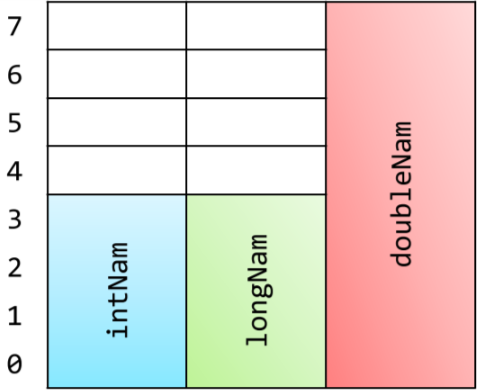
\includegraphics[width=\linewidth]{images/union.png}
\end{minipage}

\subsection{Bitfelder}

\subsubsection{Eigenschaften von Bitfeldern}
\begin{itemize}
	\item Innerhalb eines \emph{int} können einzelne Bitgruppen definiert und angesprochen werden.
	\item Sollte nicht eingesetzt werden, um damit Speicher zu sparen.
	\item Bei Embedded Systems ist der Einsatz unter Umständen sehr nützlich, wenn auf einzelne Register zugegriffen werden soll.
	\item[\-]\begin{achtung}
		Leider definiert der C++-Standard (und auch der C-Standard) nicht, ob die Bits von Links nach Rechts oder von Rechts nach Links aufgefüllt werden. Falls der Standard dies definieren würde, wären die Bitfelder ein sehr gutes Konstrukt.
	\end{achtung}
\end{itemize}

\subsubsection{Definition von Bitfeldern}
\vspace{-\baselineskip}
\begin{minipage}{0.8\linewidth}
\begin{lstlisting}
struct FieldName
{
	unsigned int a: 3;	// definiert 3 Bits fuer a
	unsigned int b: 4;	// definiert die naechsten 4 Bits fue b
	...
};
\end{lstlisting}
\end{minipage}
\begin{minipage}{0.6\linewidth}
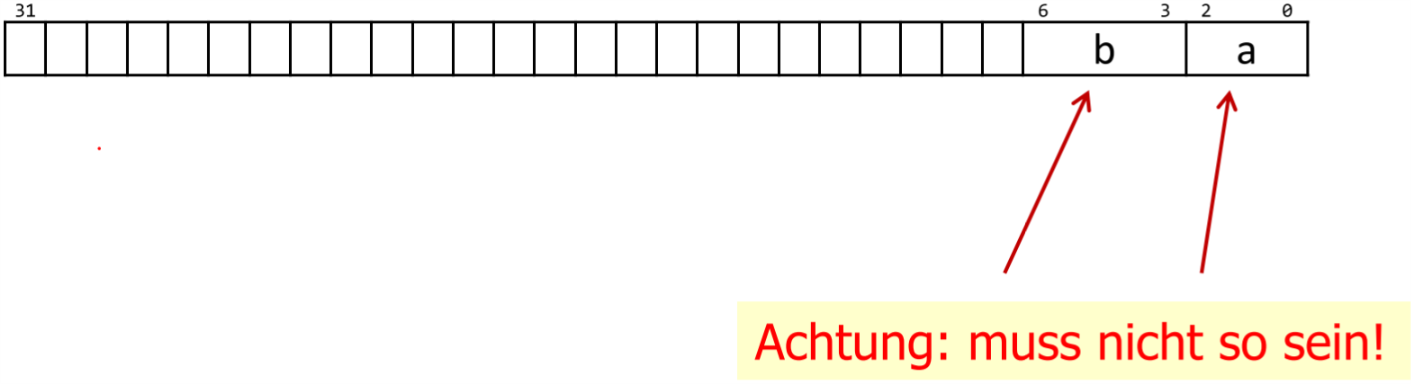
\includegraphics[width=\linewidth]{images/bitfelder.png}
\end{minipage}

\subsubsection{Bitfelder: Folgerungen}
\begin{itemize}
	\item Mit diesem Bitfeld-Mechanismus soll weder in C noch in C++ gearbeitet werden, wenn der Code portabel sein soll.
	\item Die bessere Alternative ist die Verwendung von Bitmasken-Operationen. Diese können in C++ bspw. in inline-Funktionen verpackt werden.
\end{itemize}
\vfill
\pagebreak\newpage

\section{Beispielprojekt Stack}

\begin{multicols}{2}
	\subsection{Stack}
	\begin{minipage}{0.8\linewidth}
		\begin{itemize}
			\item Der Stack ist ein oft verwendetes Speicherkonstrukt für Daten.
			\item Bei einem Stack werden neue Elemente immer oben eingefügt.
			\item Elemente werden immer auch wieder oben weggenommen.
			\item Synonyme:
			\begin{itemize}
				\item Stapel
				\item LIFO (Last In First Out)
				\item (Kellerspeicher)
			\end{itemize}
		\end{itemize}
	\end{minipage}%
	\begin{minipage}{0.2\linewidth}
		\includegraphics[width=\linewidth]{images/klasse1.pdf}
	\end{minipage}
	\vfill\null
	\columnbreak
	\subsubsection{Stack - Operationen}
	\begin{tabular}{ll}
		\hline 
		push() & ein neues Objekt einfügen \\ 
		\hline 
		pop() & ein Objekt entfernen \\ 
		\hline 
		isEmpty() & liefert true falls der Stack leer ist \\ 
		\hline 
		isFull() & liefert true falls der Stack voll ist \\ 
		\hline 
		init() & initialisiert einen leeren Stack \\ 
		\hline 
	\end{tabular}
\end{multicols}

\subsubsection{Demo: Codebeispiel für Stack (Stack\_Datenkapsel)}
\lstinputlisting{listings/Stack_Datenkapsel/stack.h}
\lstinputlisting{listings/Stack_Datenkapsel/stack.cpp}

\subsubsection{Demo: Klasse Stack}
\begin{itemize}
	\item Stack::init() durch ctor ersetzen
	\item Verhalten bei privatem Default Ctor
	\item Verhalten bei privatem Copy Ctor
	\begin{itemize}
		\item Wenn der Copy Ctor privat deklariert wird (ohne ihn zu implementieren), dann verhindert der Compiler das Kopieren von Objekten dieser Klassen
		\item Das kann in gewissen Fällen ein durchaus erwünschtes Verhalten sein
	\end{itemize}
\end{itemize}

\begin{multicols}{2}
	\subsection{Queue}
	\begin{itemize}
		\item Die Queue ist ein weiteres Speicherkonstrukt für Daten.
		\item Bei einer Queue werden neue Elemente immer am Ende (tail) eingefügt.
		\item Elemente werden immer am Anfang (head) weggenommen.
		\item Synonyme:
		\begin{itemize}
			\item Warteschlange
			\item FIFO (First In First Out)
			\item Pipe
			\item Buffer (engl.)
			\item Puffer (dt.)
		\end{itemize}
	\end{itemize}
	\vfill\null
	\columnbreak
	\subsubsection{Queue - Operationen}
	\begin{tabular}{lc}
		enqueue() / write() & ein neues Objekt hinzufügen \\ 
		\hline 
		dequeue() / read() & ein Objekt entfernen \\ 
		\hline 
		isFull() & liefert true falls die Queue voll ist \\ 
		\hline 
		isEmpty() & liefert true falls die Queue leer ist \\ 
		init() & initialisiert eine leere Queue \\ 
	\end{tabular}
	\begin{minipage}{0.7\linewidth}
		\includegraphics[width=\linewidth]{images/klasse2.pdf}
	\end{minipage}
\end{multicols}
\clearpage
%!TEX root = ProgCPP_ZF.tex

\part{Vererbung}
\label{sec:Vererbung}

\section{Motivation}
\label{sec:Motivation}
Sie müssen einen Webshop entwickeln. Sie verkaufen Bücher und CDs.\\
Welche Eigenschaften und Methoden benötigen Sie, um ein Buch bzw. eine CD zu charakterisieren?

\section{Artikel als Gemeinsamkeit von Buch und CD}
\label{sec:Artikel als Gemeinsamkeit von Buch und CD}

%%% Bild einfügen %%%

\section{Grundkonzept}
\label{sec:Grundkonzept}
\begin{itemize}
	\item Die Vererbung erlaubt, neue Klassen auf der Basis von bestehenden Klassen zu definieren. Dabei erbt (übernimmt) die neue (Unter-)Klasse alle Eigenschaften der bestehenden (Über-)Klasse.
	\item Man sagt auch, die Oberklasse sei eine Basisklasse, Superclass, Abstraktion oder Generalisierung (Verallgemeinerung).
	\item Die Unterklasse wird auch mit Subclass oder als Spezialisierung bezeichnet.
\end{itemize}

\section{Einsatz der Vererbung}
\label{sec:Einsatz der Vererbung}
\begin{itemize}
	\item Bestehende Klassen erweitern
	\begin{itemize}
		\item zusätzliche Attribute erweitern
		\item zusätzliche Elementfunktionen
	\end{itemize}
	\item Bestehende Methode einer Basisklasse ändern (überschreiben)
	\item Das Finden von guten Basisklassen ist eine Hauptaufgabe in der Designphase.
\end{itemize}

\section{UML-Notation}
\label{sec:UML-Notation}
\begin{itemize}
	\item Generalisierung/Spezialisierung
	\item SubClass erbt sämtliche Eigenschaften von SuperClass
	\item ist-ein Beziehung (SubClass \textbf{ist eine} SuperClass)
	\item Pfeilspitze ist ein geschlossenes Dreieck
\end{itemize}

%%% Bild Folie 8 einfügen %%%

\subsection{"ist ein"-Beziehung}
\label{sec:"ist ein"-Beziehung}
"ist ein"-Beziehung ("is a"-relationship)\\
Beispiel: Baum \textbf{ist eine} Pflanze, Blume \textbf{ist eine} Pflanze.

\section{Beispiel: Vererbungshierarchie Lebewesen}
\label{sec:Beispiel: Vererbungshierarchie Lebewesen}

%%% Bild Folie 10 einfügen %%%

\subsection{C++-Syntax}
\label{sec:C++-Syntax}
\noindent
\begin{minipage}{\linewidth}
	\begin{lstlisting}
	class SubClass *@\color{red}: public SuperClass\color{black}@*
	{
		public:
		
		protected:
		
		private:
		
	};
	\end{lstlisting}
\end{minipage}
public ist Normalfall (private und protected sind auch möglich).

\subsection{Zugriff auf Elemente der Basisklasse}
\label{sec:Zugriff auf Elemente der Basisklasse}

%%% Bild Folie 12 %%%

\section{Spezifikation von Basisklassen}
\label{sec:Spezifikation von Basisklassen}
\begin{itemize}
	\item Grundsatz: Vererbung sollte immer public sein (zu 99,99\%)
	\item Falls bei Vererbung protected oder private in Betracht gezogen wird, kann der Grund dafür eine falsche Verwendung der Vererbung sein
	\item Für ganz spezifische Anwendungen kann die Vererbung mit protected oder private sinnvoll sein
\end{itemize}

\section{Beispiel: ComicCharacter (Comics01)}
\label{sec:Beispiel: ComicCharacter (Comics01)}

%%% Comics01 einfügen
%%% Bild (Klassen) von Folie 14


\section{Einsatz von protected bei Klassenelementen}
\label{sec:Einsatz von protected bei Klassenelementen}
\begin{itemize}
	\item Bei Datenelementen (Attributen) soll protected grundsätzlich nicht eingesetzt werden. Attribute sollen generell private sein.
	\item Bei Elementfunktionen kann es in Einzelfällen sinnvoll sein, diese als protected zu definieren. Dadurch wird der Zugriff gegenüber einer public-Sichtbarkeit auf die abgeleiteten Klassen beschränkt.
\end{itemize}

\section{Objektgrösse bei der Vererbung}
\label{sec:Objektgrösse bei der Vererbung}
\begin{itemize}
	\item Ein Objekt einer vererbten Klasse enthält alle Teile der Basisklasse(n) und zusätzlich noch die spezifischen eigenen Teile.
	\item Das Objekt ist somit mindestens so gross wie jenes der Basisklasse(n). (es gibt keine Vererbung "by reference")
	\item Wenn Vererbung schlecht eingesetzt wird (z.B. keine is-a-Beziehung), können unnötig grosse Objekte entstehen.
	\item Bei einer Aggregationsbeziehung kann durchaus eine Referenz (oder ein Pointer) auf ein anderes Objekt verwendet werden, d.h. Aggregation "by reference" ist möglich.
\end{itemize}

\section{Schlechter (falscher) Einsatz von Vererbung}
\label{sec:Schlechter (falscher) Einsatz von Vererbung}
Zwischen Wald und Pflanze besteht nicht eine "ist-ein" Beziehung. Die richtige Beziehung wäre "hat-ein", da ein Wald mehrere Pflanzen hat (folgt später).

%%% Bild Folie 17

\section{Substitutionsprinzip}
\label{sec:Substitutionsprinzip}
\begin{itemize}
	\item Ein Objekt einer Oberklasse kann Objekte einer beliebigen Unterklasse aufnehmen.
	\item Ein Objekt einer Unterklasse kann keine Objekte der Oberklasse aufnehmen.
	\item[\-]
	\noindent
	\begin{minipage}{\linewidth}
		\begin{lstlisting}
		class SuperClass{}; 
		
		class SubClass : public SuperClass {};
		
		SuperClass super;
		SubClass sub;
		super = sup; 	*@\color{green}// ok\color{black}@"
		sub = super;	*@\color{red}// geht nicht \color{black}@*
		\end{lstlisting}
	\end{minipage}
\end{itemize}













\clearpage
%!TEX root = ProgCPP_ZF.tex

\part{Polymorphismus}
\textbf{Auftrag:} Stellen Sie bei allen Uhren die Zeit eine Stunde vor.
\begin{itemize}
	\item Obwohl der Auftrag völlig klar ist, hat man Mühe ihn auszuführen, weil jede Uhr auf eine andere Art verstellt wird.
	\item Der Auftrag ist recht abstrakt, die Ausführung ist aber sehr konkret, sobald sie wissen, welche Uhr sie verstellen müssen
\end{itemize}

\section{Static vs. Dynamic Binding}
\begin{itemize}
	\item Static Binding (early binding, statische Bindung)
	\begin{itemize}
		\item bereits zur Compilezeit wird festgelegt, welcher (Elementfunktions-) Code ausgeführt wird (Normalfall)
	\end{itemize}
	\item Dynamic Binding (late binding, dynamische Bindung)
	\begin{itemize}
		\item erst zur Laufzeit wird in Abhängigkeit des Objekts festgelegt, welcher (Elementfunktions-) Code ausgeführt wird
		\item Analogie: sobald sie wissen, welche Uhr sie verstellen müssen, können sie das konkrete Verfahren anwenden
		\item das ist das Konzept des Polymorphismus
	\end{itemize}
\end{itemize}

\subsection{Dynamic Binding}
\begin{itemize}
	\item ist der mächtigste OO-Mechanismus (oft präziser mit run-time polymorphism bezeichnet)
	\item Elementfunktionen, die dynamisch gebunden werden, muss bei der Deklaration das Schlüsselwort \textbf{virtual} vorangestellt werden (zwingend!)
	\begin{itemize}
		\item in der abgeleiteten Klasse soll (muss aber nicht) die Funktion auch mit virtual gekennzeichnet werden
	\end{itemize}
	\item Polymorphismus wird häufig als ineffizient bezeichnet, oft jedoch zu unrecht (mehr darüber im Vertiefungsmodul Embedded Software Engineering)
	\item Regeln:
	\begin{itemize}
		\item Eine Funktion soll dann als \textbf{virtual} deklariert werden, wenn sie in der abgeleiteten Klasse neu definiert (überschrieben) wird, sonst nicht! In diesem Fall muss auch der Destruktor \textbf{virtual} sein.
		\item Der Destruktor muss auch dann \textbf{virtual} sein, wenn ein Objekt einer Unterklasse dynamisch erzeugt wird und einem Pointer auf die Basisklasse zugewiesen wird (Substitutionsprinzip).
	\end{itemize}
	\item Achtung: nicht mit Funktionsüberladung (gleicher Name aber unterschiedliche Signatur) verwechseln!
\end{itemize}

\subsubsection{Beispiel: Zeichnen von geometrischen Figuren}
\begin{itemize}
	\item Eine immer gleich heissende Elementfunktion draw() hat unterschiedliche Implementationen, je nach Art des aktuellen Objekts.
	\item Bsp.: Eine Zeichenfunktion für geometrische Objekte hat ganz unterschiedliche Implementationen, je nach dem ob es sich um einen Kreis, ein Rechteck, Textblock, Polygonzug, etc. handelt.
\end{itemize}

\subsection{Statischer vs. dynamischer Datentyp}
\noindent
\begin{minipage}{\linewidth}
	\begin{lstlisting}
	class Article;
	class Book : public Article {};
	Article* pa;
	pa = new Book;
	\end{lstlisting}
\end{minipage}
\begin{itemize}
	\item Der statische Datentyp bezeichnet den Datentyp bei der Deklaration $\rightarrow$ pa ist ein pointer auf Article
	\item Der dynamische Datentyp bezeichnet den effektiven Datentyp zur Laufzeit $\rightarrow$ pa ist ein Pointer auf Book
\end{itemize}

\subsection{Aufruf von virtuellen Elementfunktionen}
\label{sec:aufrufVonVirtuellenElemenfunktionen}
\begin{itemize}
	\item Virtuelle Elementfunktionen können sowohl dynamisch (über Pointer oder Referenzen) als auch statisch aufgerufen werden.
	\item Bei statischen Aufrufen erfolgt die Auswahl der richtigen Funktion bereits bei der Übersetzung (d.h. ohne Overhead)
	\begin{itemize}
		\item Dies ist dann der Fall, wenn das Objekt bereits zur Entwicklungszeit bekannt ist.
	\end{itemize}
	\item Bei dynamischen Aufrufen erfolgt die Auswahl der richtigen Funktion zur Laufzeit aufgrund des tatsächlichen (dynamischen) Typs des Objekts. Dies ist mit einem Overhead verbunden.
\end{itemize}

\subsubsection{Statischer Aufruf von virtuellen Elementfunktionen}
\noindent
\begin{minipage}{\linewidth}
	\begin{lstlisting}
	Duck donald;
	SuperHero luckyLuke;
	
	donald.print();		// Duck::print()
	luckyLuke.print();	// SuperHero::print()
	\end{lstlisting}
\end{minipage}

\subsubsection{Dynamischer Aufruf von virtuellen Elementfunktionen}
\noindent
\begin{minipage}{\linewidth}
	\begin{lstlisting}
	void printCC1(const ComicCharacter& c)
	{
		c.print();	// dynamische Aufloesung
	}
	
	void printCC2(const ComicCharacter* pc)
	{
		pc->print();	// dynamische Aufloesung
	}
	
	Duck donald;
	SuperHero luckyLuke;
	printCC1(donald);	// Duck::print()
	printCC2(&luckyLuke);	// SuperHero::print()
	\end{lstlisting}
\end{minipage}

\subsection{Polymorphe Klassen (Virtuelle Klassen)}
\begin{itemize}
	\item Eine Klasse, welche mindestens eine virtuelle Funktion deklariert, heisst virtuell (polymorph)
	\item Virtuelle Klassen bewirken einen Mehraufwand für den Compiler und sind darum langsamer in der Ausführung
	\item Funktionen sollten nur dann als virtuell deklariert werden, wenn sie in einer abgeleiteten Klasse überschrieben werden (sollen)
	\item Konstruktoren sind nie virtuell
	\item Destruktoren virtueller Klassen müssen immer als virtuell deklariert werden, sonst wird nur der Destruktor der Basisklasse aufgerufen
	\item Destruktoren müssen auch dann virtuell sein, wenn ein Heapobjekt über einen Pointer der Basisklasse freigegeben wird
	\item Nicht virtuelle Methoden dürfen nicht überschrieben werden	
\end{itemize}

\subsubsection{Repräsentation virtueller Objekte im Speicher}
\begin{minipage}{0.45\linewidth}
	\begin{itemize}
		\item In der Virtual Function Table (vtbl) vermerkt das System der Reihe nach die Adressen der für eine Klasse gültigen virtuellen Elementfunktionen
		\item Das System legt für jede polymorphe Klasse eine vtbl an
		\item Jedes Objekt einer polymorphen Klasse enthält einen Virtual Table Pointer (vptr), welcher auf die vtbl der entsprechenden Klasse zeigt
	\end{itemize}
\end{minipage}
\begin{minipage}{0.5\linewidth}
	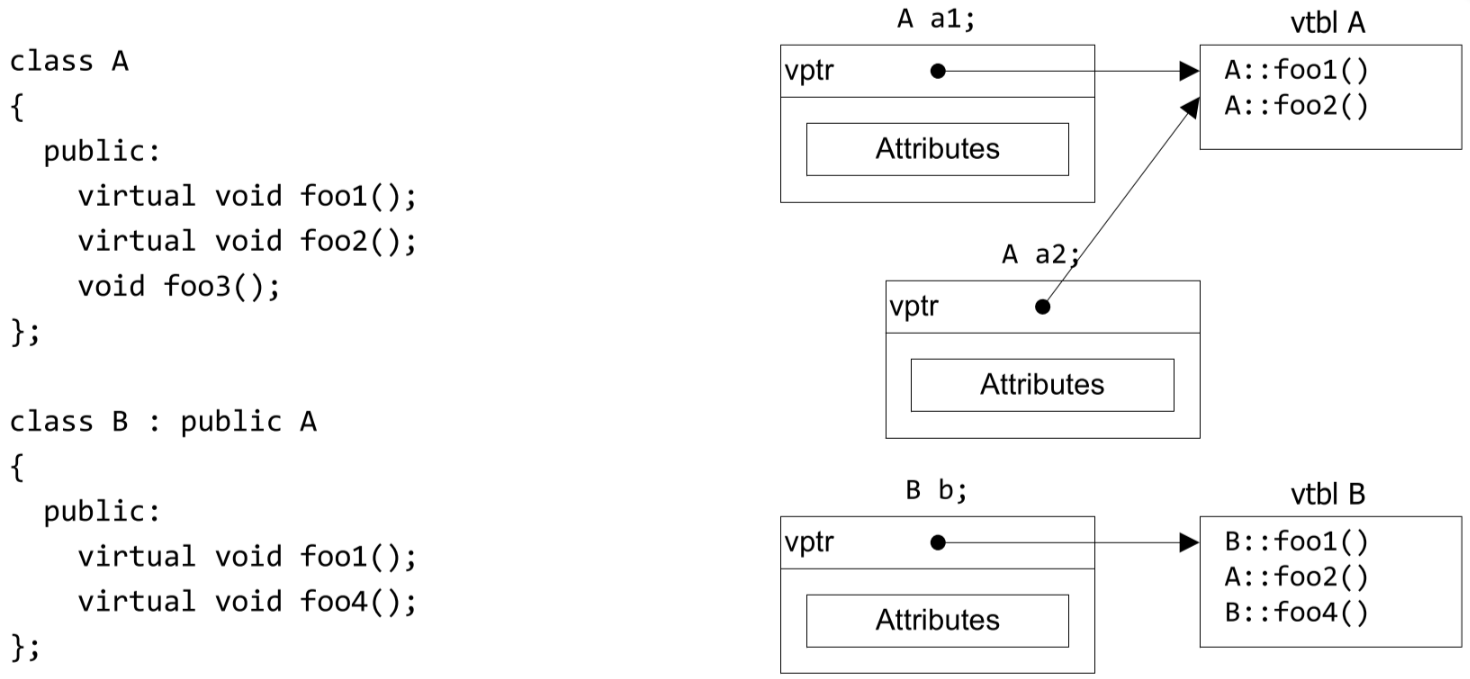
\includegraphics[width=\linewidth]{images/vtbl.png}
\end{minipage}

\section{Abstrakte Klassen}
\begin{itemize}
	\item Für manche Situationen sind die Vererbungsmechanismen, die wir bisher kennen gelernt haben, nicht ausreichend.
	\item Ein Kreis ist z.B. ein Spezialfall einer Ellipse. Es ist aber nicht sinnvoll, ihn so zu programmieren, da er sonst Eigenschaften erbt, die nicht verwendet werden.
	\item Es wäre möglich, Kreis und Ellipse als zwei unabhängige Klassen zu programmieren. Dann müssten aber alle Eigenschaften, die diese gemeinsam haben, doppelt programmiert werden.
	\item Dies versucht die objektorientierte Programmierung zu vermeiden.
	\item Es ist besser, die Eigenschaften, die Kreise und Ellipsen gemein haben, in einer Basisklasse zu programmieren.
	\item Die Kreis- und Ellipsenklassen erben dann parallel von der gemeinsamen Basisklasse.
	\item Die Basisklasse ist aber unvollständig, es handelt sich um eine abstrakte Klasse.
	\item Es können keine Objekte von abstrakten Klassen gebildet werden.
	\item In C++ können rein virtuelle Funktionen (pure virtual functions) deklariert werden, die in der Basisklasse nicht von einer Definition begleitet werden.
	\item Klassen, die mindestens eine rein virtuelle Funktion deklarieren, sind abstrakte Klassen
	\item Ist eine Klasse erst einmal als abstrakt definiert, kann diese nur durch Vererbung vervollständigt und dadurch nutzbar gemacht werden.
\end{itemize}

\subsection{Anwendungen von abstrakten Klassen (Beispiele)}
\begin{itemize}
	\item Definition von Schnittstellen (Interfaces)
	\begin{description}
		\item[Abstrakte Kommunikationsklasse] SerialCom, USB, Ethernet, etc. können davon sein
		\item[Abstrakte Printerklasse] Jeder Printertreiber erbt davon, bzw. implementiert dieses Interface. Die Hauptapplikation (z.B. Word) muss nicht geändert werden, wenn ein neuer Printertreiber implementiert wird.
	\end{description}
	\item "Real nicht existierende Abstrahierungen"
	\begin{itemize}
		\item ...von denen es keinen Sinn macht, ein Objekt zu erzeugen.
		\item Geometrische Figur als Gemeinsamkeit von Kreis, Rechteck, etc.
	\end{itemize}
\end{itemize}

\section{Mehrfachvererbung (Multiple Inheritance, MI)}
\begin{itemize}
	\item Manchmal ist es sinnvoll, eine abgeleitete Klassen von mehreren verschiedenen Basisklassen erben zu lassen.
	\item Wir sprechen dann von Mehrfachvererbung.
	\item Bei der Mehrfachvererbung werden die Basisklassen durch Komma getrennt:
	\subitem \textbf{class SingingWaiter : public Waiter, public Singer}
	\item Bei den Konstruktoren (Chaining) müssen die Konstruktoren der Basisklassen in der Ordnung gelistet werden, in der sie aufgerufen werden sollen.
\end{itemize}
\begin{multicols}{2}
	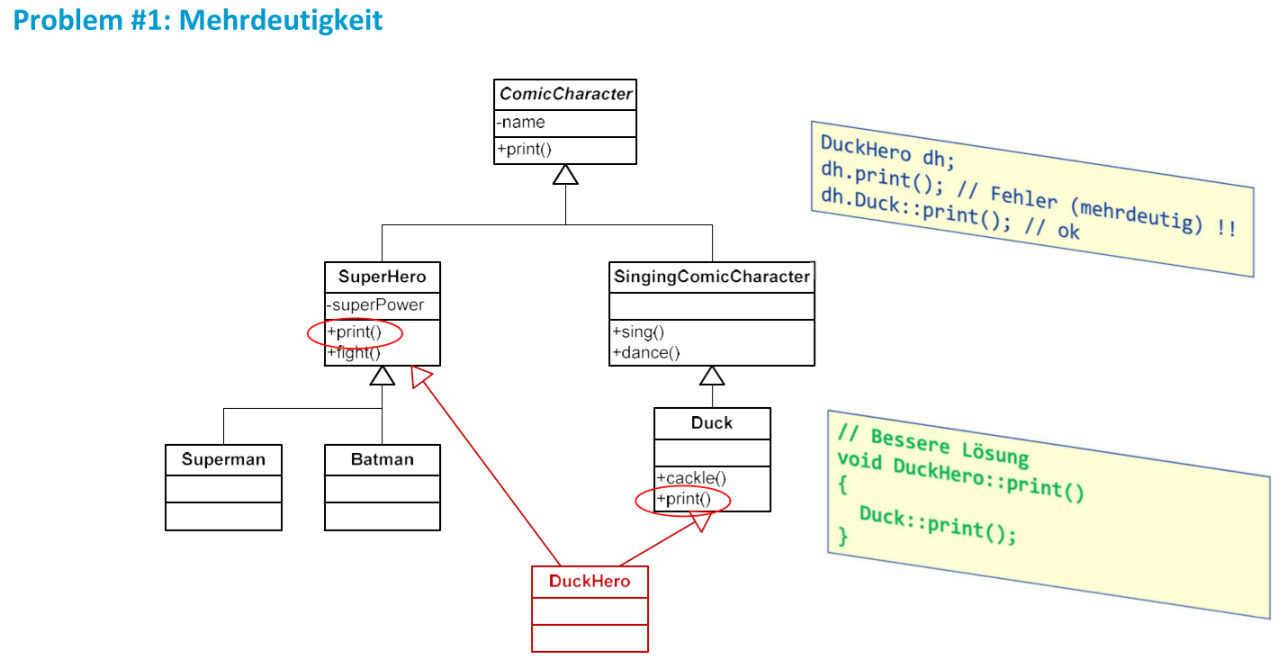
\includegraphics[width=\linewidth]{images/mehrdeutigkeit.png}
	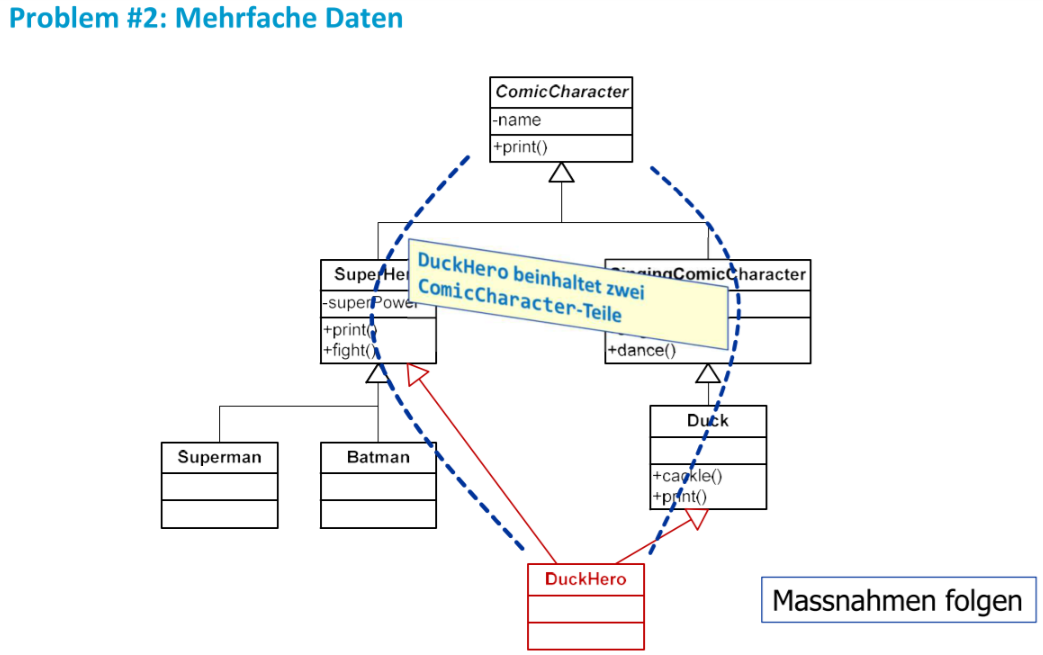
\includegraphics[width=\linewidth]{images/mehrfacheDaten.png}
\end{multicols}
\begin{itemize}
	\item Mehrfachvererbung ist ein sehr mächtiges Konzept, das (richtig eingesetzt) sehr nutzbringend sein kann. Bei schlechtem Einsatz der Mehrfachvererbung können enorme Probleme eingehandelt werden.
	\item Ein "guter" Einsatz der Mehrfachvererbung ist, wenn alle ausser höchstens einer Basisklasse ausschliesslich aus rein virtuellen Funktionen bestehen (Interfaces). Die neue Klasse implementiert dann die aufgelisteten Interfaces.
	\item Das ist die Art "Mehrfachvererbung", die auch in Java vorhanden ist: Vererbung gibt es nur einfach mit extends plus beliebige Implementationen von einem bis mehreren Interfaces mit implements
\end{itemize}

\subsection{Virtuelle Basisklassen}
Um zu vermeiden, dass bei Mehrfachvererbung eine gemeinsame Basisklasse mehrfach im Speicher vorkommt, kann virtuell geerbt werden.
\noindent
\begin{minipage}{\linewidth}
	\begin{lstlisting}
	class SingingComicCharacter : virtual public ComicCharacter
	{
		...
	};
	
	class SuperHero : virtual public ComicCharacter
	{
		...
	};
	\end{lstlisting}
\end{minipage}
In der Klasse DuckHero muss als erstes der ComicCharacter-Konstruktor aufgerufen werden.

\section{Laufzeit-Typinformationen (Run-Time Type Information, RTTI)}
\begin{itemize}
	\item Wie kann der (dynamische) Type eines polymorphen Objekts ermittelt werden?
	\item RTTI heisst der Mechanismus und \textbf{steht ausschliesslich für polymorphe Klassen zur Verfügung}
	\item Operator dynamic\_cast
	\item Operator typeid
	\item Struktur type\_info
\end{itemize}
\begin{achtung}
	RTTI sollte nur äusserst zurückhaltend eingesetzt werden!
\end{achtung}
\begin{itemize}
	\item Einsatz z.B. bei persistenten Objekten (um z.B. auch Klasseninformationen in einer rationalen Datenbank abzuspeichern)
\end{itemize}

\subsection{Operator dynamic\_cast}
\begin{itemize}
	\item Syntax: dynamic\_cast<SuperHero*>(p)
	\item Versucht, den Zeiger p in eine Zeiger auf ein Objekt des Typs SuperHero umzuwandeln.
	\item Der dynamische Datentyp von p ist massgebend.
	\item Umwandlung wird dann durchgeführt, wenn p tatsächlich auf ein Objekt vom Typ SuperHero, bzw. auf eine davon abgeleitete Klasse zeigt.
	\begin{itemize}
		\item Andernfalls ist das Resultat der Umwandlung der Nullpointer!
	\end{itemize}
\end{itemize}

\subsection{Operator typeid}
\begin{itemize}
	\item Ermitteln des dynamischen Datentyps eines polymorphen Objekts
	\item Ergibt eine Referenz auf ein Objekt des Typs type\_info. Diese Klasse beinhaltet u.a. eine Methode name(), welche den Namen der Klasse zurückgibt.
	\item Beispiel:
	\subitem cout << $"$p ist ein $"$ << typeid(*p).name() << $"$Objekt$"$;
\end{itemize}




\clearpage
%%!TEX root = ProgCPP_ZF.tex

\part{Templates}
\label{sec:Templates}

\section{Generische Programmierung mit Templates (Schablonen)}
\label{sec:Generische Programmierung mit Templates (Schablonen)}

\subsection{Motivation für Templates}
\label{sec:Motivation für Templates}
\begin{itemize}
	\item Viele Algorithmen sollten für unterschiedliche Datentypen implementiert werden
	\item Die Algorithmen unterscheiden sich kaum oder gar nicht von Typ zu Typ
	\item Beispiele:
	\begin{itemize}
		\item In einem Stack sollten verschiedene Typen abgespeichert werden können (int, double, char,...)
		\item Wenn für einen bestimmten Typ eine Ordnungsrelation (<) definiert ist, dann kann die Sortierung von solchen unterschiedlichen Typen mit einem einzigen Algorithmus implementiert werden
	\end{itemize}
\end{itemize}

\subsection{Lösung mit bekannten Techniken}
\label{sec:Lösung mit bekannten Techniken}
\begin{itemize}
	\item Für jeden Typ müsste eine eigene Version implementiert werden
	\begin{itemize}
		\item Dies ergibt eine grosse Anzahl von fast identischem Code
		\item Alle Implementationen müssen getestet werden
		\item Bei grundlegenden Korrekturen müssen alle Implementationen korrigiert werden
	\end{itemize}
	\item Eine (durchaus mögliche) "generische" C-Variante mit void* hat keine Typprüfung
\end{itemize}

\subsection{Generische Programmierung mit Templates}
\label{sec:Generische Programmierung mit Templates}
\begin{itemize}
	\item Single Source-Prinzip: ein bestimmtes Problem (Algorithmus) wird nur einmal unabhängig vom Typ gelöst
	\item Template-Definitionen erzeugen grundsätzlich noch keine einzige Zeile Code. Erst wenn das Template wirklich verwendet wird, wird Code für diesen Typ erzeugt.
	\item Templates sind somit für Bibliotheken ideal geeignet
	\item Traditionelle Bibliotheken belegen Speicher unabhängig davon, ob eine einzelne Funktion wirklich verwendet wird. Dies kann zu Dead Code führen, d.h. zu Code, der niemals ausgeführt wird.
\end{itemize}

\section{Funktions-Templates}
\label{sec:Funktions-Templates}
\begin{itemize}
	\item Templates verwenden den Typ als "Variable"
	\item Die Algorithmen können unabhängig vom Typ (generisch) implementiert werden
	\begin{achtung} Templates sind keine Funktionsdefinitionen, sie beschreiben dem Compiler nur, wie er den Code definieren soll, d.h. der Compiler nimmt den konkret verwendeten Typ, setzt diesen in das Template ein und compiliert den so erhaltenen Code.
	\end{achtung}
	\item Die Bindung zum konkreten Typ geschieht bereits zur Compiletime (early binding), sobald erkannt ist, mit welchem Typ das Template aufgerufen (benutzt) wird.
\end{itemize}

\subsection{Syntax für Funktions-Templates}
\label{sec:Syntax für Funktions-Templates}
\begin{itemize}
	\item Vor den Funktionsnamen wird das Schlüsselwort template, gefolgt von einer in spitzen Klammern eingeschlossenen Parameterliste gestellt.
	\item Die Parameterliste enthält eine (nicht leere) Liste von Typ- und Klassenparametern, die mit dem Schlüsselwort class oder typename beginnen. (typename ist zu bevorzugen).\\
	Die einzelnen Parameter werden mit Komma getrennt.
\end{itemize}
\noindent
\begin{minipage}{\linewidth}
	\begin{lstlisting}
	template<typename A, typename B>
	int foo(A a, B b, int i);
	
	template<typename Any> // or class Any
	void swapIt(Any\& a, Any\& b);
	
	template<typename ElemType>
	ElemType minimum(ElemType elemField[], int fieldSize);
	\end{lstlisting}
\end{minipage}

\subsection{Beispiel (aus Prata): Zwei Werte vertauschen}
\label{sec:Beispiel (aus Prata): Zwei Werte vertauschen}
\lstinputlisting{\listings/templateSwap.cpp}

\subsection{inline bei Templates}
\label{sec:inline bei Templates}
\noindent
\begin{minipage}{\linewidth}
	\begin{lstlisting}
	template<typename Any>
	inline void swapIt(Any\& a, Any\& b)
	{
		Any temp;	// temp a variable of type Any
		temp = a;
		a = b;
		b = temp;
	}
	\end{lstlisting}
\end{minipage}
inline muss zwischen template und dem Returntyp stehen.
\begin{achtung}
Bei Verwendung von inline speziell zusammen mit Templates besteht die Gefahr von Code Bloat. Nur bei sehr kurzen Funktionen verwenden.	
\end{achtung}

\subsection{Beispiel: kleinstest Element finden}
\label{sec:Beispiel: kleinstest Element finden}
\noindent
\begin{minipage}{\linewidth}
	\begin{lstlisting}
	template<typename ElemType>
	ElemType minimum(const ElemType elemField[], int size);
	
	template<typename ElemType>
	ElemType minimum(const ElemType elemField[], int size)
	{
		int min = 0;	// Index des kleinsten Elementes
		for(int i=1; i<size; ++i)
		{
			if(elemField[i] < elemField[min])
				min = i;
		}
		return elemField[min];
	}
	\end{lstlisting}
\end{minipage}
\begin{achtung}
Der Operator < muss für jeden verwendeten Typ definiert sein.
\end{achtung}

\subsection{Ausprägung von Funktions-Templates}
\label{sec:Auspraegung von Funktions-Templates}
\begin{itemize}
	\item Sobald ein Typ in einem Funktions-Template verwendet wird, erkennt der Compiler, dass es sich um ein Template handelt und prägt es für diesen Typ aus (implizite Ausprägung).
	\noindent
	\begin{minipage}{\linewidth}
		\begin{lstlisting}
		int iF[] = {1, 54, 34, 23, 67, 4};
		int i = minimum(iF, sizeof(iF)/sizeof(iF[0]));
		\end{lstlisting}
	\end{minipage}
	\item Für die Auflösung werden nur die Funktionsparameter betrachtet, der Rückgabetyp wird nicht ausgewertet.
\end{itemize}

\subsection{Explizite Qualifizierung von Funktions-Templates}
\label{sec:Explizite Qualifizierung von Funktions-Templates}
\begin{itemize}
	\item Funktions-Templates können explizit mit einem Typ qualifiziert werden
	\noindent
	\begin{minipage}{\linewidth}
		\begin{lstlisting}
		int iF[] = {1, 54, 34, 23, 67, 4};
		int i = minimum<int>(iF, sizeof(iF)/sizeof(iF[0]));
		\end{lstlisting}
	\end{minipage}
	\item Mögliche Anwendungen: siehe Strasser s.233
\end{itemize}

\subsection{Überladen von Funktions-Templates}
\label{sec:Ueberladen von Funktions-Templates}
\begin{itemize}
	\item Funktions-Templates können mit anderen Funktionstemplates und auch mit "normalen" Funktionen überladen werden
	\begin{hinweis}
	überladen = gleicher Funktionsname, unterschiedliche Parameterliste
	\end{hinweis}
	\item Namensauflösung
	\begin{itemize}
		\item Compiler geht die Liste der möglicherweise passenden Funktions-Templates durch und erzeugt die entsprechenden Template-Funktionen
		\item Ergebnis ist eine Reihe von (eventuell) passenden Template-Funktionen, ergänzt durch die vorhandenen "normalen" Funktionen
		\item Aus dieser ganzen Auswahl wird die am besten passende Funktion ausgewählt
	\end{itemize}
\end{itemize}

\section{Klassen-Templates}
\label{sec:Klassen-Templates}

\subsection{Definition: Klassen-Template}
\label{sec:Definition: Klassen-Template}
\begin{itemize}
	\item Klassen-Templates sind mit Typen oder Konstanten parametrisierbare Klassen
	\item Im Gegensatz zu Funktions-Templates können in Klassen-Templates auch die Attribute der Klassen mit variablen Typen ausgestattet sein
	\item Ein Klassen-Template kann auch von Ausdrücken abhängig sein. Diese Ausdrücke müssen aber zur Compiletime aufgelöst werden können
	\begin{itemize}
		\item Diese Möglichkeit kann gerade in Embedded Systems sehr nützlich sein
	\end{itemize}
\end{itemize}

\subsection{Syntax für Klassen-Templates}
\label{sec:Syntax fuer Klassen-Templates}
\begin{itemize}
	\item Die Syntax ist analog zu den Funktions-Templates.
	\item Vor die Klassendeklaration wird das Schlüsselwort template, gefolgt von einer in spitzen Klammern eingeschlossenen Parameterliste gestellt.
	\item Die Parameterliste enthält eine (nicht leere) Liste von Typ- und Klassenparametern, die mit dem Schlüsselwort class oder typename (typename bevorzugen) beginnen oder auch von Ausdrücken.
	\item Die einzelnen Parameter werden mit Komma getrennt.
\end{itemize}

\subsubsection{Beispiel zu Klassen-Template: Deklaration}
\label{sec:Beispiel zu Klassen-Template: Deklaration}
\noindent
\begin{minipage}{\linewidth}
	\begin{lstlisting}
	template<typename ElemType, int size=100>
	class Stack
	{
		public:
			Stack();
			~Stack();
			void push(const ElemType\& elem);
			ElemType pop();
			bool wasError() const;
			bool isEmpty() const;
		private:
			ElemType elems[size];
			int top;
			bool isError;
	};
	\end{lstlisting}
\end{minipage}

\subsubsection{Beispiel zu Klassen-Template: Definition}
\label{sec:Beispiel zu Klassen-Template: Definition}
\noindent
\begin{minipage}{\linewidth}
	\begin{lstlisting}
	template<typename ElemType, int size>
	void Stack<ElemType, size>::push(const ElemType\& elem)
	{
		// implementation goes here
	}
	\end{lstlisting}
\end{minipage}
Die Syntax scheint bei der Definition etwas umständlich...

\subsubsection{Beispiel zu Klassen-Template: Nutzung (Ausprägung)}
\label{sec:Beispiel zu Klassen-Template: Nutzung (Auspraegung)}
\noindent
\begin{minipage}{\linewidth}
	\begin{lstlisting}
	Stack<int, 10>	s1;	// s1 ist ein Stack mit 10 int
	Stack<int>		s2;	// s2 ist ein Stack mit 100 int (Default)
	Stack<double>	s3;	// s3 ist ein Stack mit 100 double
	\end{lstlisting}
\end{minipage}
...Die Syntax ist für die Nutzung genial einfach.

\subsection{Bemerkungen}
\label{sec:Bemerkungen}
\begin{itemize}
	\item Mit den Templates haben sie die Möglichkeit, auf Sourcecode-Ebene Elemente mit variablem Typ und variabler Grösse zu definieren, z.B.
	\noindent
	\begin{minipage}{\linewidth}
		\begin{lstlisting}
		Stack<int, 10>	s1;
		\end{lstlisting}
	\end{minipage}
	\item Die variable Stackgrösse 10 wird dabei nicht durch eine dynamische Allozierung auf dem Heap erreicht, sondern durch Einsetzen dieses Wertes im Template (Templateparameter size).
	\item Dadurch wird ein Array der Grösse 10 \textbf{vom Compiler} erzeugt. Dies ist sehr effizient.
\end{itemize}

\subsection{Explizite Ausprägung von Klassen-Templates}
\label{sec:Explizite Auspraegung von Klassen-Templates}
Klassen-Templates können analog zu den Funktions-Templates explizit mit einem Typ qualifiziert werden
\noindent
\begin{minipage}{\linewidth}
	\begin{lstlisting}
		tenplate<typename KeyType, typename ElemType>
		class Map
		{
			...
		}
		
		class Map<int, TString>;
		// Der Compiler praegt nun diese Kombination explizit aus
	\end{lstlisting}
\end{minipage}

\subsection{Klassen-Templates und getrennte Übersetzung: export}
\label{sec:Klassen-Templates und getrennte Uebersetzung: export}
\begin{achtung}
	Ab dem Standard C++11 wird export nicht mehr unterstützt!
\end{achtung}
\begin{itemize}
	\item Falls ein Template auch in anderen Übersetzungseinheiten benutzt wird, muss dieses Template bei der Deklaration mit dem Schlüsselwort export gekennzeichnet werden
	\noindent
	\begin{minipage}{\linewidth}
		\begin{lstlisting}
		export template<class ElemType, int size>
		class Stack
		{
			...
		};
		\end{lstlisting}
	\end{minipage}
\end{itemize}

\subsection{Klassen-Templates und getrennte Übersetzung}
\label{sec:Klassen-Templates und getrennte Uebersetzung}
\begin{itemize}
	\item Für diese Aufgabe muss eine etwas unschöne Methode gewählt werden.
	\item Ein Template besteht wie andere Funktionen/Klassen auch aus einer Deklaration und einer Definition. Beim Template entsteht aus der Definition aber nicht direkt Objektcode, sondern sie ist nur eine Codeschablone.
	\item Deshalb muss jede Clientdatei des Templates sowohl die Deklaration als auch die Definition inkludieren. Der Compiler muss die Definition des Templates zwingend kennen.
	\item In der nachfolgend gezeigten Variante muss weiterhin nur die Headerdatei durch die Clients inkludiert werden.
\end{itemize}

\subsubsection{File-Organisation \#1 bei Klassen-Templates}
\label{sec:File-Organisation \#1 bei Klassen-Templates}
\lstinputlisting{\listings/stack1.h}
\lstinputlisting{\listings/stack1.cpp}
\lstinputlisting{\listings/client1.cpp}

%%% Files erstellen %%%

\begin{achtung}
	Mögliche Probleme: stack.cpp darf nicht "normal" compiliert werden. Eine IDE wie Eclipse nimmt allenfalls alle *.cpp-Files in ihren Compile-Prozess. stack.cpp muss davon ausgeschlossen werden.
\end{achtung}

\subsubsection{Ausschliessen eines cpp-Files von Compilierung in Eclipse}
\label{sec:Ausschliessen eines cpp-Files von Compilierung in Eclipse}
%%% Bild einfügen %%%


\subsubsection{File-Organisation #2 bei Klassen-Templates}
\label{sec:File-Organisation #2 bei Klassen-Templates}
\lstinputlisting{\listings/stack2.h}
\lstinputlisting{\listings/client2.cpp}

%%% Files erstellen %%%

\begin{hinweis}
Sowohl die Deklaration als auch die Definition des Templates sind im File stack.h vorhanden. Dadurch gibt es keine Probleme mit IDEs.\\
Nachteil: Deklaration und Definition sind nicht getrennt.
\end{hinweis}

\subsection{Fazit}
\label{sec:Fazit}
Sowohl Variante #1 als auch #2 haben Vor- und Nachteile.\\
Wählen sie eine aus! (Ich bevorzuge #2)
\clearpage
%!TEX root = ProgCPP_ZF.tex

\part{Exceptions ("`Ausnahmen"')}

\section{Exception vs. Error}
Bitte unterscheiden Sie zwischen Exception (Ausnahme) und Error (Fehler)\\
\begin{itemize}
	\item \textbf{Error (Fehler):} Abweichung zur Spezifikation ($"$falsch implementiert$"$). Errors sollten bei der Verifikation (Testen) entdeckt werden.
	\item \textbf{Exception (Ausnahme):} abnormale (aber vorhersehbare und mögliche) Bedingung bei der Programmausführung.
	\item Wir sprechen hier über Exception Handling (der Ausdruck Error Handling ist aus oben genannten Gründen eigentlich falsch, obwohl er sehr häufig verwendet wird). Leider heissen auch die Standardklassen in C++ häufig xyz\_error statt xyz\_exception (schade, ist nicht einmal konsistent)
\end{itemize}

\section{Mögliche Reaktionen auf Ausnahmen}
\begin{itemize}
	\item \textbf{Ignorieren}\\
		Motto: $"$Augen zu und durch$"$ Eine sehr risikoreiche Variante!
	\item \textbf{Programmabbruch}\\
		Merkt immerhin, dass etwas nicht in Ordnung ist, die Reaktion ist aber unbefriedigend. Ist Exception Detection aber nicht eigentlich Exception Handling.
	\item \textbf{Exceptioncodes} (nicht Fehlercodes)\\
		Funktionen geben als Rückgabewert, als Parameter oder global einen Ausnahmecode an.
\end{itemize}

\subsection{Exceptioncodes als Rückgabewert}
\begin{multicols}{2}
\begin{minipage}{\linewidth}
\vspace{-2\baselineskip}
\begin{lstlisting}
if (eOk == s.push(elem))
{
	...
}
else
{
	... // handle exception
}
\end{lstlisting}
\end{minipage}
\vfill\null
\columnbreak
\begin{itemize}
	\item Rückgabewert wird von Exceptioncodes belegt (ist unschön)
	\item Geht nicht bei Konstruktoren (Ctors haben keinen Rückgabewert)
	\item Bei differenzierten Exceptioncodes gibt es stark verschachtelte if ... else bei jedem Aufruf $\rightarrow$ unleserlich
\end{itemize}
\end{multicols}

\subsection{Exceptioncodes als Referenzparameter}
\begin{multicols}{2}
\begin{minipage}{\linewidth}
	\vspace{-2\baselineskip}
\begin{lstlisting}
s.push(elem, excpt);
if (eOk == excpt)
{
	...
}
else
{
	... // handle exception
}
\end{lstlisting}
\end{minipage}
\vfill\null
\columnbreak
\begin{itemize}
	\item Aufruf wird mit zusätzlichem Referenzparameter für den Exceptioncode erweitert (ist unschön)
	\item Bei differenzierten Exceptioncodes gibt es stark verschachtelte if ... else bei jedem Aufruf $\rightarrow$ unleserlich	
\end{itemize}
\end{multicols}
\vfill
\pagebreak\newpage

\subsection{Globaler Exceptioncode}
\begin{multicols}{2}
\begin{minipage}{\linewidth}
\vspace{-2\baselineskip}
\begin{lstlisting}
s.push(elem);	// globalException is set
if (eOk == globalException)
{
	...
}
else
{
	... // handle Exception
}
\end{lstlisting}	
\end{minipage}
\vfill\null
\columnbreak
\begin{itemize}
	\item Führt aufgrund des globalen Exceptioncodes zu schwer les- und wartbaren Programmen.
	\item Bei differenzierten Exceptioncodes gibt es stark verschachtelte if ... else bei jedem Aufruf $\rightarrow$ unleserlich
\end{itemize}
\end{multicols}

\subsection{Wo sollen Exceptions behandelt werden?}
\begin{itemize}
	\item Fact: Exceptions können irgendwo im Programm entstehen
	\item Wie soll auf Exceptions reagiert werden?
	\item Eine angemessene Reaktion kann häufig nicht ausschliesslich an der Stelle des Auftretens gemacht werden
	\item Die Reaktion muss auch weiter $"$nach oben$"$ gereicht werden können, bis auf die Applikationsebene, wo allenfalls eine Mitteilung an den Benutzer getätigt wird.
	\item[\-] \begin{hinweis}
		Grundsatz: Nur das regeln, was sinnvoll ist und auf einer bestimmten Stufe wirklich entschieden werden kann, sonst nach oben weiterreichen.
	\end{hinweis}
\end{itemize}

\section{Ziel für Exception Handling}
\begin{itemize}
	\item $"$Normaler$"$ Programmablauf (Schönwetterfall) wird durch das Exception Handling nicht tangiert
	\item Der Normalfall soll einfach gelesen werden können
	\item Der Ausnahmefall ist klar und einfach geregelt
	\item Der Overhead soll möglichst klein sein
	\item Die Weiterreichung an die nächsthöhere Funktion im Call Stack soll einfach sein
\end{itemize}

\section{Exception Handling in C++}
\begin{itemize}
	\item Exceptions werden in Form eines Objekts am Ort ihres Auftretens ausgeworfen (explizit oder auch $"$automatisch$"$) (werfen = to throw)
	\item Exception Handler versuchen, diese Exception-Objekte aufzufangen (to catch)
\end{itemize}

\subsection{Exception Handling in C++: Syntax}
\begin{minipage}{\linewidth}
\vspace{-\baselineskip}
\begin{lstlisting}
try
{
	... // Code, der eine Exception auswerfen koennte
}
catch (const MyExceptionClass& exc)
{
	... // wenn ein Objekt der Klasse MyExceptionClass oder einer Unterklasse
			// davon ausgeworfen wurde, dann kann dieser Handler das Objekt fangen
}

// u.U. weitere Catches
\end{lstlisting}
\end{minipage}
\vfill
\pagebreak\newpage

\subsection{Auslösen (Werfen) von Ausnahmen}
\begin{itemize}
	\item Ausnahmen können mit dem Schlüsselwort \emph{throw} explizit ausgeworfen werden
	\item Nach einem \emph{throw-}Befehl wird das Programm abgebrochen und beim ersten passenden umgebenden Handler fortgesetzt
	\item Dabei werden alle lokalen Objekte wieder automatisch zerstört (Stack unwinding)
	\item Geworfen werden kann ein beliebiges Objekt (üblich: ein spezifisches C++-Ausnahmeobjekt)
	\item (Ausschliesslich) innerhalb eines Exception Handlers ist auch die Form\hspace{0.05\linewidth}
	\begin{minipage}{0.1\linewidth}
	\vspace{-\baselineskip}
\begin{lstlisting}
throw;
\end{lstlisting}
	\end{minipage}\\
	erlaubt. Dadurch wird die Exception an den nächsten Handler weitergereicht (Exception propagation).
\end{itemize}

\subsubsection{Beispiel für Exception Handling: unübliche Variante}
\vspace{-\baselineskip}
\begin{multicols}{2}
\begin{minipage}{\linewidth}
\begin{lstlisting}
class Xcpt
{
	public:
		Xcpt(const char* text);
		~Xcpt();
		const char* getDiagStr() const;
	private:
		const char* diagStr;
};

void allocateFoo()
{
	b1();
	if (0 == allocation())
		throw Xcpt("Allocation failed!");
	b2();
}
\end{lstlisting}
\end{minipage}
\begin{minipage}{\linewidth}
\begin{lstlisting}
// Testprogramm
void testFoo()
{
	a1();
	try
	{
		a2();
		allocateFoo();
		a3();
	}
	catch (const Xcpt& exc)
	{
		cout << "Caught exception. Text: " << exc.getDiagStr() << endl;
	}
	a4();
}
\end{lstlisting}
\end{minipage}
\end{multicols}

\begin{multicols}{2}
\subsection{Vordefinierte Ausnahmeklassen}
\begin{itemize}
	\item Ausnahmeobjekte können beliebigen Typs sein (z.B. auch \emph{int}). Meist werden jedoch spezifische hierarchisch organisierte C++-Ausnahmeklassen verwendet.
	\item Vordefinierte Standardklasse: \emph{exception}
\end{itemize}
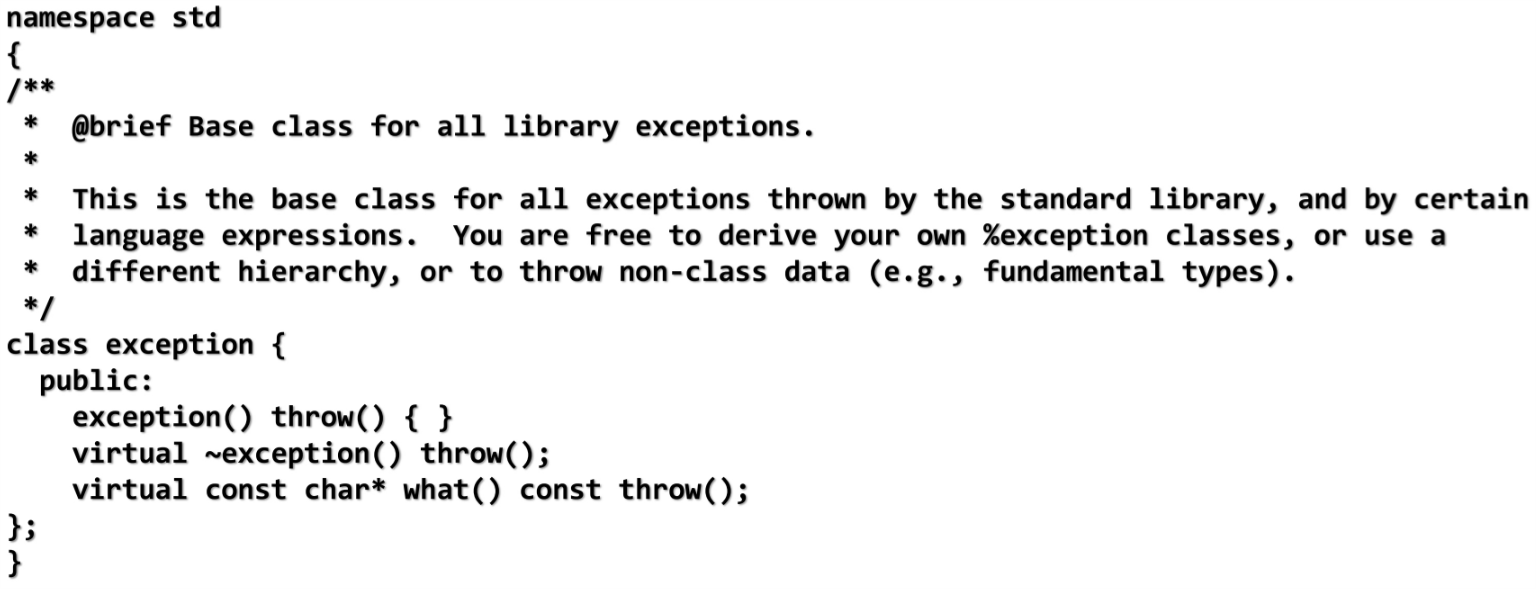
\includegraphics[width=\linewidth]{images/exceptionClass.png}
\end{multicols}

\begin{multicols}{2}
\subsection{Exception-Hierarchie in C++}
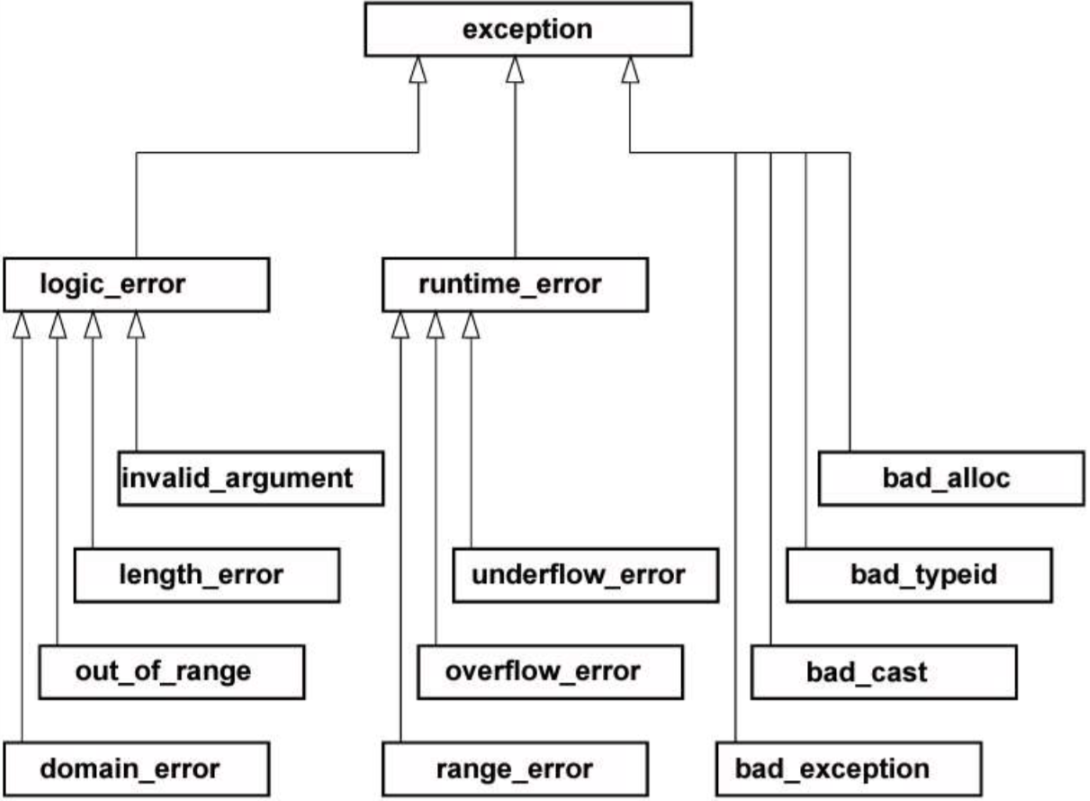
\includegraphics[width=0.8\linewidth]{images/exceptionHierarchie.png}
\vfill\null
\columnbreak
\subsection{Laufzeit- vs. Logische "`Fehler"'}
\begin{itemize}
	\item Logische "Fehler" (logic\_error)
	\begin{itemize}
		\item Ausnahmen im Programmablauf, die bereits zur Entwicklungszeit ihre Ursachen haben.
		\item Theoretisch könnten diese Ausnahmen verhindert werden.
	\end{itemize}
	\item Laufzeit"fehler" (runtime\_error)
	\begin{itemize}
		\item Nicht vorhersehbare Ausnahmen wie z.B. arithmetische Überläufe
		\item Diese Ausnahmen treten erst zur Laufzeit auf, z.B. durch eine nicht erlaubte Benutzereingabe
	\end{itemize}
\end{itemize}
\end{multicols}

\begin{multicols}{2}
\subsection{Exceptions und ihre Header-Dateien}
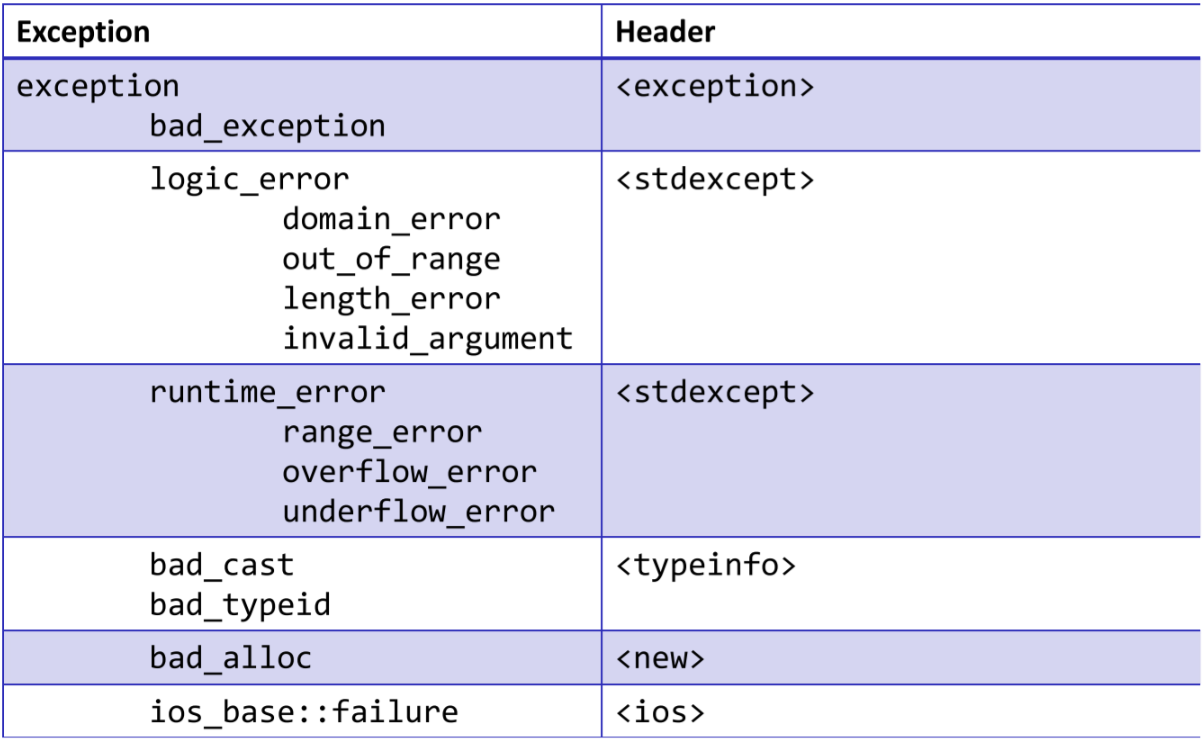
\includegraphics[width=\linewidth]{images/exceptionHeader.png}
\vfill\null
\columnbreak
\subsection{Exception Handler}
\begin{itemize}
	\item Ein oder mehrere Exception Handler können hintereinander definiert werden
	\item Die einzelnen \emph{catch}-Handler müssen sich in den Parametern unterscheiden
	\item Wenn eine Exception geflogen kommt, wird \textbf{der erste passende Handler} genommen. Ein passender Handler macht ein \emph{catch} auf genau diese Exception oder auf eine Basisklasse derselben.
	\item[\-] \begin{achtung}
	Deshalb (\textbf{sehr wichtig}): Der allgemeinste Handler (am weitesten oben in der Hierarchie) muss der letzte \emph{catch}-Handler sein.
	\end{achtung}
\end{itemize}
\end{multicols}

\subsection{Exception Handler 2}
\begin{itemize}
	\item Wenn kein Handler passt, dann wird im Aufrufstack nach oben gesucht, ob ein passender Handler vorhanden ist.
	\item Wenn auch dort keiner gefunden wird, dann wird die Funktion \emph{terminate()} aufgerufen.
	\item \emph{terminate()} beendet das Programm, kann aber auch selbst definiert werden.
	\item Catch all\\
	Der folgende Handler fängt ausnahmslos alle Exceptions ab (und muss wenn gewünscht deshalb immer als letzter aufgeführt werden):\hspace{0.05\linewidth}
	\begin{minipage}{0.15\linewidth}
	\vspace{-\baselineskip}
\begin{lstlisting}
catch(...) {}
\end{lstlisting}
	\end{minipage}
\end{itemize}

\subsection{Exception Propagation}
\begin{itemize}
	\item Innerhalb eines Exception Handlers kann eine Exception mittels\\
	\textbf{throw;}\\
	weitergereicht werden.
	\item Die Exceptiion wird dann auch nicht etwa an das nächste \textbf{catch(...)} weitergeleitet, sondern an die aufrufende Funktion.
\end{itemize}

\subsection{Exception Specification}
\begin{minipage}{0.6\linewidth}
\vspace{-\baselineskip}
\begin{lstlisting}
void foo() throw(/* Liste der Exceptions */);
\end{lstlisting}
\end{minipage}
\begin{itemize}
	\item Die Liste spezifiziert, welche Exceptions von einem Aufrufer von \emph{foo()} erwartet werden müssen.
	\item Aber: garantiert auch, dass das Programm abstürzt, wenn eine andere als eine der spezifizierten Exceptions ausgeworfen wird, d.h. \emph{foo()} muss dafür sorgen, dass wirklich nur die aufgelisteten Exceptions ausgeworfen werden.
	\item Genauer: falls eine nicht spezifizierte Exception ausgeworfen wird, dann wird die Funktion \emph{unexpected()} aufgerufen, welche üblicherweise das Programm abbricht.
	\item \emph{unexpected()} kann selbst definiert werden.
\end{itemize}
\vfill
\pagebreak\newpage

\subsubsection{Exception Specification: Beispiele}
\begin{minipage}{0.7\linewidth}
\vspace{-\baselineskip}
\begin{lstlisting}
void foo1() throw(specificXcpt1, specificXcpt2);
// die zwei angegebenen Exceptions muessen vom Aufrufer von
// foo1() erwartet werden.

void foo2() throw();
// KEINE Exceptions koennen geflogen kommen

void foo3();
// beliebige Exceptions muessen erwartet werden
\end{lstlisting}
\end{minipage}

\subsubsection{Exception Handling in der Praxis}
\begin{itemize}
	\item Exceptions sollen nur für Ausnahmen, nicht für den normalen Ablauf verwendet werden
	\item Exceptions sollen nicht vorbeugende Abfragen ersetzen
	\item Ein Programm soll nur gegen $"$entscheidende$"$ Ausnahmen abgesichert werden
	\item Wenn eine Exception ausgeworfen wird, dann wird normalerweise eine der vordefinierten Exceptionklassen oder eine (evtl. selbst definierte) Unterklasse davon genommen
	\item Exception specifications werden, wenn überhaupt, nur bei ausgewählten (Schnittstellen-)Funktionen definiert
	\item \textbf{Always throw exceptions by value, and catch them by const reference.}
\end{itemize}

\subsubsection{Handling von System Exceptions}
\begin{multicols}{2}
\begin{minipage}{\linewidth}
\vspace{-\baselineskip}
\begin{lstlisting}
int Calculator::divide()
{
	if (0 == nr2)
		throw runtime\_error("Division durch Null");
	
	return nr1 / nr2;
}
\end{lstlisting}
\end{minipage}
\vfill\null
\columnbreak
Q: In obiger Variante wird verhindert, dass überhaupt erst eine Division durch Null ausgeführt wird. Könnte die Division nicht einfach probiert werden? Das System sollte ja wenn nötig eine Runtime Exception selbständig auswerfen?
\begin{minipage}{\linewidth}
\vspace{-\baselineskip}
\begin{lstlisting}
int Calculator::divide()
{
	return nr1 / nr2;
}
\end{lstlisting}
\end{minipage}
\end{multicols}

\subsubsection{Betreibt meine Umgebung Exception Mapping?}
\begin{itemize}
	\item Mit Hilfe des folgenden Codeausschnitts kann einfach überprüft werden, ob eine bestimmte Umgebung Exception Mapping betreibt:
	\begin{minipage}{\linewidth}
	\vspace{-\baselineskip}
\begin{lstlisting}
try
{
	int a = 5;
	int b = a/0;
}
catch (...)
{
	cout << "Caught exception if exception is mapped" << endl;
}
\end{lstlisting}
	\end{minipage}
	\item Unter Umständen muss die Null über \emph{cin} (zur Laufzeit) eingegeben werden, da $"$freundliche$"$ Compiler allenfalls darauf hinweisen, dass eine Division durch Null nicht geht.
\end{itemize}
\clearpage
%!TEX root = ProgCPP_ZF.tex

\part{Preprocessor}
\label{sec:Preprocessor}

\section{Eigenschaften des Preprocessors}
\label{sec:Eigenschaften des Preprocessors}
\begin{itemize}
	\item Wird vor der eigentlichen Übersetzung aktiviert
	\item Führt textuelle Manipulationen von Source-Dateien durch
	\begin{itemize}
		\item Makro-Substitution
		\item bedingte Übersetzung
		\item Einfügen von Dateien
	\end{itemize}
	\item Der Output des Preprocessors wird dem eigentlichen Compiler übergeben
	\item Die Direktiven des Preprocessors beginnen immer mit \#
	\item Der Preprocessor ist zeilenorientiert
\end{itemize}

\section{Preprocessor-Direktiven und Bedingungsanweisungen}
\label{sec:Preprocessor-Direktiven und Bedingungsanweisungen}
\centering
\begin{tabularx}{0.5\textwidth}{|X|X|}
	\hline
	\textbf{Direktiven} & \textbf{Bedingungsanweisungen}\\
	\hline
	\#define & \#if\\
	\hline
	\#undef & \#ifdef\\
	\hline
	\#include & \#ifndef\\
	\hline
	\#line & \#elif\\
	\hline
	\#error & \#else\\
	\hline
	\#pragma & \#endif\\
	\hline
\end{tabularx}
\flushleft

\subsection{\#define}
\label{sec:define}
\begin{itemize}
	\item Definition von Makros (Gefahren betrachten!)\\
	\noindent
	\begin{minipage}{\linewidth}
		\begin{lstlisting}
		#define MAX(a,b) ((a)>(b)?(a):(b))	
		\end{lstlisting}
	\end{minipage}
	\item Definition von symbolischen Konstanten (Gefahren beachten!)\\
	\noindent
	\begin{minipage}{\linewidth}
		\begin{lstlisting}
		#define PI 3.14159265358
		\end{lstlisting}
	\end{minipage}
	\item Es erfolgt eine reine Textersetzung ohne Typenprüfung. Diese kann erst der Compiler vornehmen
	\item \#defines haben keinen Scope
	\item Simple Definition eines Symbols (z.B. bei Include-Guard)\\
	\noindent
	\begin{minipage}{\linewidth}
		\begin{lstlisting}
		#define FOO\_H\_
		\end{lstlisting}
	\end{minipage}
\end{itemize}

\subsection{\#undef}
\label{sec:undef}
Definition eines Symbols rückgängig machen
\noindent
\begin{minipage}{\linewidth}
	\begin{lstlisting}
	#undef MAX
	#undef PI
	#undef FOO_H_
	\end{lstlisting}
\end{minipage}

\subsection{\#include}
\label{sec:include}
Vollständiges Einfügen einer Datei
\noindent
\begin{minipage}{\linewidth}
	\begin{lstlisting}
	#include <iostream>
	// Datei iostream wird in den definierten Include-Verzeichnissen
	// gesucht und eingefuegt
	
	#include "foo.h"
	// Datei foo.h wird im aktuellen Verzeichnis gesucht und eingefuegt
	
	#include "../drivers/doo.h"
	// Pfadangaben muessen immer relativ zum aktuellen Verzeichnis sein.
	// Niemals absolute Pfade verwenden!
	\end{lstlisting}
\end{minipage}

\subsection{\#line}
\label{sec:line}
Direktes Setzen der Nummerierung von Sourceode-Zeilen. Durch die optionale Angabe eines Dateinamens lässt sich der Compiler einen neuen Dateinamen unterschieben.\\
Das kann z.B. bei vom Compiler erstellten Dateien nützlich sein.
\noindent
\begin{minipage}{\linewidth}
	\begin{lstlisting}
	#line 67 "main.cpp"
	// die naechste Zeile im Sourcecode erhaelt die Nummer 67
	// die Sourcedatei erhaelt den Namen "main.cpp"
	\end{lstlisting}
\end{minipage}

\subsection{\#error}
\label{sec:error}
Sofortiger Abbruch des Compiler-Vorgangs und Ausgabe einer Fehlermeldung
\noindent
\begin{minipage}{\linewidth}
	\begin{lstlisting}
	#ifndef MODEL
	#error MODEL ist nicht definiert
	#endif
	\end{lstlisting}
\end{minipage}

\subsection{\#pragma}
\label{sec:pragma}
\begin{itemize}
	\item \#pragma-Direktiven erlauben die Verwendung von Implementierungs-spezifischen Direktiven. Entwicklungsumgebungen können somit ihre eigenen Anweisungen definieren.\\
	\textbf{Diese Direktive ist damit per Definition nicht portabel.}
	\item Konflikte entstehen keine, da eine Compiler unbekannte \#pragma-Direktiven ignoriert.
	\item Die Portabilität ist damit aber nicht gewährleistet. Ein anderer Compiler versteht die Direktive u.U. nicht und erzeugt deshalb nicht den gewünschten Code.
\end{itemize}

\subsection{Bedingungsanweisungen}
\label{sec:Bedingungsanweisungen}
\begin{itemize}
	\item Bedingungsanweisungen sind nach folgendem Schema aufgebaut\\
	-----------------\\
	Bedingungsprüfung\\
	Direktiven\\
	beliebig viele \#elif-Gruppen mit Direktiven\\
	optional ein \#else mit Direktiven
	\#endif
	\item Mögliche Bedingungsprüfungen sind
	\begin{itemize}
		\item \#if gibt true, falls Bedingung true ist
		\item \#ifdef SYMBOL gibt true, falls SYMBOL definiert ist
		\item \#ifndef SYMBOL gibt true, falls SYMBOL nicht definiert ist
	\end{itemize}
\end{itemize}

\subsubsection{Beispiele für Bedingungsanweisungen}
\label{sec:Beispiele für Bedingungsanweisungen}
\noindent
\begin{minipage}{\linewidth}
	\begin{lstlisting}
	#if INT\_MAX > 32767
		int i;
	#else
		long i;
	#endif
	
	#ifdef TESTVERSION
		printf("Zeilennummer: %d\n", __LINE__);
		printf("Dateiname: %s\n", __FILE__);
	#endif
	
	#ifndef CALCULATOR\_H\_
	#define CALCULATOR\_H\_
	// ...
	#endif
	\end{lstlisting}
\end{minipage}
\noindent
\begin{minipage}{\linewidth}
	\begin{lstlisting}
	#if 0
		// Auskommentieren des gesamten hier stehenden Codes.
		// Ist sehr nuetzlich waehrend der Entwicklung.
	\end{lstlisting}
\end{minipage}

\subsection{Weitere Features des Preprocessors}
\label{sec:Weitere Features des Preprocessors}
\begin{itemize}
	\item \#-Operator (stringizing-Operator): Argument wird in String konvertiert
	\item \#\#-Operator (token-past-Operator): Zeichenfolge links und rechts des Operators wird zusammengezogen
	\item und weiteres (siehe Dokus)
	\noindent
	\begin{minipage}{\linewidth}
		\begin{lstlisting}
		#define SHOW(var, nr) printf(#var #nr " = %.1f\n", var ## nr)
		
		// Annahme: es gibt eine Variable x5 mit dem Wert 16.4
		SHOW(x, 5);
		// wird umgesetzt in printf("x" "5" " = %.1f\n", x5);
		// d.h. in printf("x5 = %.1f\n", x5);
		
		// Ausgabe ist x5 = 16.4
		\end{lstlisting}
	\end{minipage}
\end{itemize}
\textbf{na ja!?}

\subsection{Kritische Würdigung des Preprocessors}
\label{sec:Kritische Würdigung des Preprocessors}
\begin{itemize}
	\item Preprocessoranweisungen sollten zurückhaltend eingesetzt werden, da der Code durch zu viele Preprocessoranweisungen sehr schnell unübersichtlich werden kann.
	\item Auf den ersten Blick sind Preprocessoranweisungen oft nicht nachvollziehbar.
	\item Häufig gibt es Alternativen, die ebenso effizient und zudem viel sicherer sind.
	\item Richtig eingesetzt kann der Preprocessor sehr nützlich sein.
\end{itemize}
\end{document}
